\documentclass{report}

\usepackage[british]{babel}
\usepackage{lipsum} % pack�age to generate filler text Lorem Ip�sum dummy text 
\usepackage[margin=25mm,left=30mm,includefoot]{geometry} % geometry package to define margins. Possibility to make left margin larger for binding the document.

\usepackage[hidelinks]{hyperref}  % Allows for clickable reference
\hypersetup{colorlinks = true, linkcolor=blue, citecolor = {blue}, urlcolor=blue,}
\usepackage{enumitem}




% Graphics preamble
\newcommand\scalemath[2]{\scalebox{#1}{\mbox{\ensuremath{\displaystyle #2}}}}
\usepackage{graphicx} % Alows you to import images
\graphicspath{{figures/}}
\usepackage{caption}
\usepackage{subcaption}
\usepackage{float} % Allows for control of float positions

\usepackage{booktabs}

% Header and Footer Stuff
\usepackage{fancyhdr}   % package for extensive control of page headers and footers
\pagestyle{fancy}
\fancyhead{}
\fancyfoot{}
\fancyfoot[R]{\thepage\ }
\renewcommand{\headrulewidth}{0pt}    % Removes beautiful line in header
\renewcommand{\footrulewidth}{1pt}
\usepackage[bottom]{footmisc}  % keeps footnotes at bottom of page
\usepackage{multirow}

% Bibliography preamble
\usepackage[round]{natbib}

% Math preamble
\usepackage[short]{optidef} % Why is this package not working?
\usepackage{amsmath,amssymb,amsthm,mathtools,bm,etoolbox, cases, commath}
\newtheorem{myax}{Axiom}[chapter]
\newtheorem{mydef}{Definition}[chapter]
\newtheorem{myth}{Theorem}[chapter]
\usepackage{algorithm}
\usepackage {algpseudocode}
\usepackage{cases}

\begin{document}

\begin{titlepage}
	\begin{center}	      % center text
	\line(1,0){300} \\     % double backslash: next line
	[2mm]                     % create space between horizontal black line and next line
	\huge{\bfseries Stochastic Correlation Modeling and Value-at-Risk Estimation by Multivariate GARCH and Machine Learning } \\  
	[2mm]
	\line(1,0){300} \\	
	\textsc{\Large Thesis Project} \\
	[5cm]
	\textsc{\LARGE Eindhoven University of Technology} \\
	[8cm]
	\end{center}
	\begin{flushleft}
	\textsc{\large P.G. Melkert \\
	0893899 \\
	September, 2017 \\
	Supervisor 1: dr. A. Chockalingam \\
	Supervisor 2: dr. R.J. Almeida}
	\end{flushleft}
\end{titlepage}

% Front matter: stuff in front of table of contents (toc)

\pagenumbering{roman}

\section*{Abstract}    % Asterisk is to remove header numbering (and toc)
\addcontentsline{toc}{section}{\numberline{}Summary}  % Gets summary in toc
"In this paper, we propose the first KNN and RF for modeling time-varying correlations of financial market returns and to improve moving window correlation estimates. The methods capture time varying correlation and conditional volatility without an underlying restricted statistical model for the correlations. " \\

\noindent
In this paper we propose an estimator of the conditional covariance matrix in a quantitive finance setting. Based on the estimation of conditional correlations using machine learning algorithms, this methodology provides an efficient estimator from a semi parametric point of view. \\


\noindent
"In this paper we show that (parsimonious) machine learning models can be used to model unobserved time-varying pairwise correlations between a set of financial market returns, where the obtained pairwise
correlations lead to a multivariate volatility model with time-varying properties. The proposed methods avoid strong distributional assumptions on the correlation process and uses the conventional approximation of time-varying correlation, namely sample correlations from exponentially weighted moving windows, as input and output variables. The input space of the machine learning models is reduced through defining the minimum and maximum past correlation as indicators of the overall correlation pattern in the market". We carried out numerical experiments based on financial market returns that show the applicability of the proposed machine learning estimation methods in specific practical situations. "A comparison was carried out with respect to another standard and parsimonious multivariate conditionally heteroscedastic family, namely, Dynamic Conditional Correlation." \\


Stochastic correlation forecasts are evaluated within the context of risk management. \\


"More accurate models of risk, as the ones proposed in this paper, can lead to better assessment and understanding of held portfolios and market exposure. The performance of VaR models is evaluated by using an unconditional coverage test (Kupiec test) and an independence test (Christoffersen Markov test)". It is (hopefully) found that the DCC-GARCH model is sometimes rejected, while the machine learning models of VaR are never/ less frequently  ejected.




         


\cleardoublepage 


% Table of Contents stuff
\tableofcontents
\thispagestyle{empty}   % removes page numbering and footer from content page 
\cleardoublepage          % clears the rest of the page

% List of figures, list of tables
\listoffigures
\addcontentsline{toc}{section}{\numberline{}List of Figures}
\cleardoublepage

\listoftables
\addcontentsline{toc}{section}{\numberline{}List of Tables}
\cleardoublepage


% Main body stuff
\pagenumbering{arabic}
\setcounter{page}{1}     % set Introduction as page 1



%NEW CHAPTER 
\chapter{Introduction}\label{sec:intro} 
"Correlations are critical inputs for many of the common tasks of � financial management. Hedges require estimates of the correlation between the returns of the assets in the hedge. If the correlations and volatilities are changing, then the hedge ratio should be adjusted to account for the most recent information. Similarly, structured products such as rainbow options that are designed with more than one underlying asset have prices that are sensitive to the correlation between the underlying returns. A forecast of future correlations and volatilities is the basis of any pricing formula.

Asset allocation and risk assessment also rely on correlations; however, in this case a large number of correlations is often required. Construction of an optimal portfolio with a set of constraints requires a forecast of the covariance matrix of the returns. Similarly, the calculation of the standard deviation of today's portfolio requires a covariance matrix of all the assets in the portfolio. These functions entail estimation and forecasting of large covariance matrices, potentially with thousands of assets.

The quest for reliable estimates of correlations between � financial variables has been the motivation for countless academic articles and practitioner conferences and much Wall Street research. Simple methods such as rolling historical correlations and exponential smoothing are widely used. More complex methods, such as varieties of multivariate generalized autoregressive conditional heteroskedasticity (GARCH) or stochastic volatility, have been extensively investigated in the econometric literature and are used by a few sophisticated practitioners. To see some interesting applications, examine the work of Bollerslev, Engle, and Wooldridge (1988), Bollerslev (1990), Kroner and Claessens (1991), Engle and Mezrich (1996), Engle, Ng, and Rothschild (1990), Bollerslev, Chou, and Kroner (1992), Bollerslev, Engle, and Nelson (1994), and Ding and Engle (2001). In very few of these articles are more than � five assets considered, despite the apparent
need for bigger correlation matrices. In most cases, the number of parameters in large models is too big for easy optimization. 

In this article, dynamic conditional correlation (DCC) estimators are proposed that have the flexibility of univariate GARCH but not the complexity of conventional multivariate GARCH. These models, which parameterize the conditional correlations directly, are naturally estimated in two steps? a series of univariate GARCH estimates and the correlation estimate. These methods have clear computational advantages over multivariate GARCH models in that the number of parameters to be estimated in the correlation process is independent of the number of series to be correlated. Thus potentially very large correlation matrices can be estimated. 

In this article, the accuracy of the correlations estimated by a variety of methods is compared in bivariate settings where many methods are feasible. An analysis of the performance of the DCC methods for large covariance matrices was considered by Engle and Sheppard (2001). 

Section 2 gives a brief overview of various models for estimating correlations. Section 3 introduces the new method and compares it with some of the cited approaches. Section 4 investigates some statistical properties of the method. Section 5 describes a Monte Carlo experiment and results are presented in Section 6. Section 7 presents empirical results for several pairs of daily time series, and Section 8 concludes." (Engle, 2001)

"Financial markets respond to information virtually instantaneously. Each new piece of information influences the prices of assets and their correlations with each other, and as the system rapidly changes, so too do correlation forecasts. This fast-evolving environment presents econometricians with the challenge of forecasting dynamic correlations, which are essential inputs to risk measurement, portfolio allocation, derivative pricing, and many other critical financial activities." \\

\noindent
"Understanding and quantifying dependence is at the core of all modelling efforts in financial econometrics. The linear correlation coefficient (Pearson correlation coefficient), which is the far most used measure to test dependence in the financial community and also elsewhere, is only a measure of linear dependence. This means that it is a meaningful measure of dependence if asset returns are well represented by an elliptical distribution. Outside the world of elliptical distributions, however, using the linear correlation coefficient as a measure of dependence may lead to misleading conclusions. In financial markets, there is often a non-linear dependence between returns." \\

\noindent
"This leads us to another potential problem?it is not always the case that the matrix composed of the pairwise converted Kendall $\tau$ values is itself a valid correlation matrix. Correlation matrices have to be positive semidefinite. A correlation matrix is simply a scaled covariance matrix and the latter must be positive semidefinite as the variance of a random variable must be non-negative."


\begin{enumerate}
	\item What can we say about the performance of the ml models using simulated data and compare the results with MW and EMW estimates of correlation? (Compare on MAE but in plots with correlations estimates also show variation of these estimates!!)
	\item Moreover, what can we say about the sensitivity of these machine learning algorithms with respect to the window size of the (exponentially weighted) moving window estimates for correlation?
\end{enumerate}

\noindent
Answer setup to question 1, 2: simulate bivariate asset process with a predefined time-varying correlation structure using Cholesky factorization. From this asset process, generate datasets with proxies (EMW estimates) for input variables and true correlations for the output variables. \\

We illustrate the model capabilities using synthetic datasets exhibiting different data properties (and subsequently real data on asset returns). \\

\noindent
"In our empirical illustration for a portfolio of 15 U.S. financial assets, the parameter estimates
imply that the realized measures receive more weight than the outer-product of the vector of
daily returns. We confirm that the realized measure is a more accurate measure of the covariance
matrix as it exploits intra-day high-frequency data. In an out-of-sample study we show that
our modeling framework can lead to accuracy improvements in forecasting, especially those for
the density in daily returns."

  

\bigskip
Why use KNN? \\
knn takes some (weighted) average of the closest n observations. For KNN, whose correlations estimates are (weighted) averages of other correlation estimates, i.e. we won't need extrapolation but require correlation estimates to fall in the interval [-1, 1]. Lazy classifiers are most useful for large datasets with few attributes (as is the case with us). Reason for this: The disadvantages with lazy learning include the large space requirement to store the entire training dataset. 


\bigskip
Why use random forest? 
\noindent
Stock data is inherently non linear in nature \\
Random Forests can learn highly irregular data\\
Random Forests can classify large amounts of data with high accuracy\\
Random Forests are natural candidate for parallelization since it comprise of highly de-correlated decision trees.\\
Random Forests converge as the number of trees in the ensemble increase. \\
They don't do well at all when you require extrapolation outside of the range of the dependent (or independent) variables. But this is exactly what we want! We want correlation estimates to fall in the interval [-1, 1]. 

note use of: MultiOutputRegressor(RandomForestRegressor())

\bigskip
Two important things to note:
1) Everything falls and stands with how well the covariate predict the output variable. So feature engineering is very important: which proxies to be used for correlation estimates? \\

 
\noindent
2) During the modelling process we should keep two things in mind: 1) Always check for/ ensure correlation matrix is symmetric and positive-semidefinite and 2) a model should be a good balance between accurateness and complexity.

\smallskip

Always: natural trade-off between capturing time variation in correlations and obtaining an accurate proxy for correlation at a given time. \\

\noindent
Density estimation: \\
Conditional density estimation makes it possible to quantify and visualize the uncertainty associated with the prediction of a continuous target variable. Given an observed vector of attribute values, a conditional density estimator provides an entire density function for the target variable, rather than a point estimate consisting of a single value. This function can then be visualized, or it can be summarized in prediction intervals that contain the true target value with a certain pre-specified probability. \\

Now, these density functions are obviously unknown for real-world data. However, if they were available, we could use them to quantify predictive uncertainty, e.g. in the form of prediction intervals. The aim of conditional density estimation is to accurately estimate conditional density functions like these.



\section{Problem Statement}
Good decisions and good modelling need comprehensive and reliable data. \\

\noindent
State difficulties in asset return correlation modeling:
\begin{enumerate}
	\item Correlation is not directly observable: solve with approximations but this introduces an error. 
	\item High dimensionality: a portfolio with $n$ stocks has dimensionality $d = n(n-1)/2$ pairwise correlations.
	\item Requirement of positive semi-definiteness. Always check requirement is satisfied after obtaining parameters.   
	\item Existing models impose additional restrictions on/ rely on distributional assumptions on the process being forecasted, i.e. correlation process. 
\end{enumerate}

\noindent
This paper is intended to address the last deficiency by clearly defining... machine learning gives us an approach that enables us to extract correlation information without relying on any distributional assumptions on the process being forecasted, i.e. the correlation process. "This is important in most applications in economics where any kind of  distributional assumption is highly questionable. In value-at-risk (VAR) applications,
 the underlying returns series is nonstationary by construction, since the portfolio is  typically changing over time. Furthermore, VAR forecasts are often plagued by  misspecification due to time-varying covariances and options risk approximations, so  that abstaining from distributional assumptions is crucial \citep{ref:Christoffersen1998}." 


\section{Research Objectives}
"The goal of this paper is to propose a simple approach to modeling multivariate volatility. The proposed model is kept parsimonious in parameterization to overcome the difficulty of curse of dimensionality." In addition, no distributional assumption is made on the correlation dynamics, i.e. no structure equation is imposed. Consequently, the proposed model is very flexible. On the other hand, lack of imposed structure does not guarantee the resulting time-varying covariance matrices are positive semi-definite such that this must be verified with obtained parameters.  \\

\noindent
We show that the KNN and RF applications improve over the conventional moving window approximation of time-varying correlation by decreasing the sensitivity of the results to the selection of the window length. \\




\section{Outline and Contributions}
We present the first KNN and RF application where estimation and forecasting capability of
these algorithms is assessed based on point forecasts of time-varying correlations. Furthermore, we will analyze the function approximation capabilities of KNN and RF under different parameterizations and report the effect of parameterizations on the accuracy of the obtained function approximation. \\

\textit{We start with a comprehensive review of the algorithms at the core of k-nearest neighbors and random forests. We discuss the learning capabilities of these models and carefully study all parts of the algorithm and their complementary effects. In particular, Chapter 4 includes original contributions on the bias-variance analysis of ensemble methods, highlighting how randomization can help improve performance. Chapter 5 concludes this first part with an original space and time complexity analysis of k-nearest neighbors and random forests (and 4 introduction their variants)}. \\

\noindent
The efficacy of this approach is assessed in a robust empirical evaluation using data of daily returns for 300 NYSE highly capitalized companies in the period between \textbf{??} and \textbf{??}. \\

"At the heart of DTP lies a unique, layered risk management approach. Managing money starts by not losing too much. While that may be easy in normal market circumstances, it is the extreme events that really matter!" \\

"DTP has a demonstrated ability to perform well in times of market stress, such as the Dot-com Collapse (2001-2002), the Credit Crisis (2007-2008) and the Brexit Referendum (2016)." \\

\noindent
Goal of the simulation part is to see if proposed learning algorithms are useful to try and whether the effect of different parameterizations on the bias-variance decomposition still holds when the output variable incorporate errors because they are approximated. 




\chapter{Nearest neighbors and Random Forests}
In this section some theoretical background is given of the learning algorithms that lie at the core of k-nearest neighbors and random forests.

\section{Nearest neighbors} \label{sec:knn}  
\begin{itemize}
	\item type algorithm: lazy learner/ instance based. Relate time + space complexity to this fact.
	\item underline simplicity of the algorithm + reason why used. Mention (break down of) performance in higher dimensions because thats second part of the analysis, i.e. curse of dimensionality. 
	\item pseudocode.
	\item time + space complexity.
	\item Mention k optimization parameter. Mention possibility of different weighting functions and distance measures. 
\end{itemize}

\noindent
The k-nearest neighbors algorithm (henceforth KNN) is a simple nonparametric learning algorithm. The algorithm makes a decision by identifying the $k$ nearest neighbors that share the highest similarity with the unseen sample instance. In this work, Euclidian distance is used as a metric for similarity. That is, the distance between two data points x$_i$ and x$_j$ is defined as follows: 

\begin{equation} \label{eq:distanceFunction}
	d(x_i,x_j) = \sqrt{\sum_{m=1}^{n} (x_{i,m} - x_{j,m})^2} 	
\end{equation} 

\noindent 

where d(x$_i$, x$_j$) is the Euclidian distance between data points x$_i$ and x$_j$, x$_{i,k}$ is the mth covariate value of x$_i$, x$_{j,m}$ is the mth covariate value of x$_j$.   \\

In this work it is preferred to discriminate between the k nearest neighbors when making predictions, i.e. let the closest observation among the k nearest neighbors have more say in affecting the outcome of the unseen sample instance. Therefore, a parameterization of KNN is considered where each of the k nearest neighbors has a weight induced from its distance with respect to the unseen sample instance. More precisely, each of the k nearest neighbors has a weight equal to the inverse of its distance to the unseen sample instance, i.e. inverse distance weighting, that is, a simple inverse distance weighting function as defined by \cite{ref:Shepard1968}: \\

\noindent
Let the training dataset be denoted by T$_{train} = {(x_1, y_1), (x_2, y_2), \cdots, (x_N, y_N)}$, $x_i = (x^1_i, x^2_i, \cdots, x^d_i) \in$ X, y$_i \in \mathbb{R}$. Let s = (x$_0$) denote an unseen sample instance and $y_0$ its prediction. The adapted inverse distance weighting function is shown in Eq. \ref{eq:IDWfunction}.

\begin{align} \label{eq:IDWfunction}
	y_0 = \frac{\sum_{i=1}^{K}w_i y_i}{\sum_{i=1}^{K}w_i} 
\end{align}
where
 
\begin{numcases} {w_i = } \nonumber
	0 & if $d(x_0, x_i) \neq 0 \wedge \exists j \neq i: d(x_0, x_j) = 0$    \\ \nonumber
    	1 & if  $d(x_0, x_i) = 0 \wedge \exists j \neq i: d(x_0, x_j) = 0$  \\ \nonumber 
    	1/d(x_0, x_i) & otherwise
\end{numcases}


The feature weighted k-nearest neighbor algorithm with inverse distance weighting is described in pseudocode by \hyperref[alg:FWKNN]{Algorithm\ 1}. The space complexity of the FWKNN algorithm is dominated by the space required by the data structure storing the training data set and thus the space complexity is O(dN). The time complexity of the FWKNN algorithm is dominated by the first for-loop. Inside the first for-loop, the distance between the sample instance and each training set instance is computed where each distance computation requires O(d) time and is done for all $N$ training instances. Hence the worst case run time for computing all distances, D$^w$, is O(dN). The arithmetic operations in the second for-loop run in constant time for $K$ times and thus the worst-case run time for the second for-loop is O(K). Selecting the K-closest neighbors can be done in O(N) time with introselect algorithm or in O(N) \textit{expected} time with randomized quick-select. If the latter is used, the worst-case run time of the FWKNN algorithm is technically O(N$^2$) because randomized quick-select runs in O(N$^2$) time \citep{ref:Goodrich2015}. The complexity analysis is based on an implementation of the FWKNN algorithm from scratch without the use of Ball tree or KD tree data structures. \\ 

% FWKNN Algorithm
\begin{algorithm}[H]
	\caption{FWKNN(T$_{train}$, s, K)}
	\label{alg:FWKNN}
	\begin{algorithmic}[1]
		\State $D^w \gets \emptyset$ \Comment{Initialize list of feature weighted distances as an empty list of size $\abs{T}$}
		\State $T_{K} \gets \emptyset$ \Comment{Initialize list of k-nearest neighbors as an empty list of size $\abs{K}$} 
		\State $y_0 \gets 0$ \Comment{Initialize the response variable to zero}
		\ForAll{$t=(x_i, y_i) \in T_{train}$}		
			\State $d^w(x_0,x_i) = \sqrt{\sum_{k=1}^{n} P_k \cdot (x_{0,k} - x_{i,k})^2}$ \Comment{Compute feature weighted distance }
			\State $D^w \gets D^w \cup (d^w(x_0,x_i), y_i)$   \Comment{Add tuple feature weighted distance and response variable}
		\EndFor		
		\State $T_{K} \gets D^w.getMin(K)$ \Comment{Assign K-smallest data tuples from D$^w$ w.r.t. $d^w(x_0,x_i)$}
		\If{$\text{$d(x_0, x_1) \in T_{K}$ is not 0}$} \Comment{Confirm existence of neighbor with zero distance}
			\State $w_i = \frac{1}{d(x_0, x_i)}$	   
		\Else
			\For{$i \in \{1, \cdots, K$\}} \Comment{Compute weights for K closest neighbors}
				\If{$\text{$d(x_0, x_i)$ is 0}$}
					\State $w_i = 1$
				\Else
					\State $w_i = 0$		
				\EndIf
			\EndFor
		\EndIf
		\State $y_0 = \frac{\sum_{i=1}^{K}w_i y_i}{\sum_{i=1}^{K}w_i}$ 		
	\State \Return $y_0$
\end{algorithmic} 
\end{algorithm}


 
From the pseudocode of the FWKNN algorithm we observe that the hyperparameter K, the number of nearest neighbors, is to be specified. The optimal value for K is specified by a grid search in the range of one to an upper boundary such as fifty or maybe even a hundred. 



\section{Random Forests}
\begin{itemize}
	\item type algorithm: ensemble learner based on two algorithms: simple learner algorithm (e.g. decision tree) and bootstrap aggregating algorithm + random feature selection. 	
	\item we can further reduce estimator variance by attempting to decorrelate the trees. This is where the notion of RANDOM Forest comes from.
	\item pseudocode.
	\item time + space complexity.
	\item based on low bias, high variance base model and bagging: implies accuracy improvement through variance reduction. Explain how from bagging an ID estimator is constructed.  
	\item mention applicability in higher dimensions through core algorithm step "random feature selection", which is nice way to address high dimensionality on optimization based strategies: d/3 for regression. 
\end{itemize}

\noindent
Randomization in random forest is achieved through 1) Bootstrap samples and 2) Random selection of split variables.

"Bagging and other resampling techniques can be used to reduce the variance in model predictions. In bagging (Bootstrap Aggregating), numerous replicates of the original data set are created using random selection with replacement. Each derivative data set is then used to construct a new model and the models are gathered together into an ensemble. To make a prediction, all of the models in the ensemble are polled and their results are averaged. \\

One powerful modeling algorithm that makes good use of bagging is Random Forests. Random Forests works by training numerous decision trees each based on a different resampling of the original training data. In Random Forests the bias of the full model is equivalent to the bias of a single decision tree (which itself has high variance). By creating many of these trees, in effect a "forest", and then averaging them the variance of the final model can be greatly reduced over that of a single tree. In practice the only limitation on the size of the forest is computing time as an infinite number of trees could be trained without ever increasing bias and with a continual (if asymptotically declining) decrease in the variance." \\

\noindent
The expectation for random forest is based on the bias-variance tradeoff. For instance, if I have $n$ independent samples from some probability distribution with mean $\mu$ and variance $\sigma$, and the samples are averaged, the newly obtained bias remains mean $\mu$. However, the newly obtained variance will be reduced to $\frac{\sigma}{n}$. \\

\noindent
\textit{In general if my samples have some correlation $\rho$, the reduction in variance depends on the correlation (a low correlation means a big reduction in variance)! This is all math. Now, suppose you have a way to generate a model which has low bias and high variance. The canonical example of this is supposedly a deep decision tree, though I?m not aware of any math showing that decision trees have low bias. Then if you can 'average' 100 models generated in the same way, then your final model should have the same bias (mean), but lower variance! Because of the bias-variance decomposition, this means that it's BETTER (the overall error is lower!). Yay! Further, the amount of variance reduction you get depends on the correlation between the 100 models. This is why random forests work! Random forests take a bunch of decision trees (low bias, high variance), average them (lower variance!). And they use an extra trick (select a random subset of features when splitting) to reduce the correlation between the trees (extra lower variance!!!). Understanding why ensembles work is awesome, it means that if an ensemble method isn't helping you, you can understand why! It's probably because the correlation between the models in your ensemble is too high.} \\

The more features you use in the decision tree construction process, the more likely the decision trees in the random forest will all do the same thing. They will more likely find the same set of feature and value to split on. \\

\noindent
\textbf{A Random Forest Guided Tour - Biau and Scornet, 2015. Good information on random forests in plain terms.} \\
Aside from being simple to use, the method is generally recognized for its accuracy and its ability to deal with small sample sizes and high-dimensional feature spaces. At the same time, it is easily parallelizable
and has therefore the potential to deal with large real-life systems....  J. Howard (Kaggle) and M. Bowles
(Biomatica) claim in Howard and Bowles (2012) that ensembles of decision trees?often known as ?random forests??have been the most successful general-purpose algorithm in modern times, while H. Varian, Chief Economist at Google, advocates in Varian (2014) the use of random forests in econometrics... \\

\noindent
\textbf{Extremely randomized trees - Geurts, 2006}
Random Forests (RF). This algorithm has been proposed by Breiman (2001) as an
enhancement of Tree Bagging. To build a tree it uses a bootstrap replica of the learning sample,
and the CART algorithm (without pruning) together with the modification used in the Random
Subspace method. At each test node the optimal split is derived by searching a random
subset of size K of candidate attributes (selected without replacement from the candidate
attributes). Empirical studies have shown that Random Forests significantly outperform Tree
Bagging and other random tree ensemble methods in terms of accuracy. In terms of degree of
randomization, this algorithm is stronger than Tree Bagging, specially if K is small compared
to the number of attributes, n. It is also stronger than Random Subspace since it combines this
method with bootstrap sampling. Randomization is both implicit (attribute and cut-point)
and explicit (attribute). We use the notation $RF^K$, with $K = d$ for the default setting, and
$K = ?$ for the best result over the range $K = 1, ... , n$. \\


\noindent
\textbf{PARALLEL tree construction does NOT result in speed up because our dataset of
1000-1500 rows is simply TOO SMALL to win increased overhead involved in multicore processing when number of trees is 100. From 1000 trees parallel processing does seem to
increase computational time.}



\chapter{Correlation Estimation using Machine Learning}

\iffalse
\https://www.google.nl/search?q=why+would+we+care+about+distributional+form+of+correlation+matrix&rlz=1C5CHFA_enNL708NL708&oq=why+would+we+care+about+distributional+form+of+correlation+matrix&aqs=chrome..69i57.10191j0j7&sourceid=chrome&ie=UTF-8
\fi

"Correlation structure among stocks in a given portfolio is a complex structure represented numerically
in the form of a symmetric matrix where all diagonal elements are equal to 1 and the off-diagonals are
the correlations of two different stocks. That matrix is the so-called correlation matrix [1]. It is clear
that the larger the number of stocks, the higher the complexity of that structure and the harder it is
to understand [2]. From recent literature such as, for example, [1?3] we learn that understanding orrelation structure is one of the most important problems in econophysics. Theoretically, correlation
matrix among stocks is a random matrix [4]. The vital importance of random matrix in this field is very
well known. Its role can be found not only in stock market analysis but also in many other areas such
as, for example, portfolio optimization [5,6], asset price [7] and ex-ante optimal portfolios [8]." \\

\noindent
In this work the following model is considered for an arbitrarily $k$ returns $y_t = (y_{1,t}, \dots, y_{k,t})'$:

\begin{align} 
	y_t = H^{1/2}_t z_t \label{eq:returns_model}
\end{align}

\noindent
where $t \in \{1, \dots,T\}$ indicates the time period, $z_t$ is a $k \times 1$ vector of i.i.d random variables with mean zero and unit variance, $H_t$ is a $k\times k$ positive definite matrix, and $H_t^{1/2}$  denotes the Cholesky decomposition of $H_t$. \\

\noindent
The time-varying variance-covariances of returns $y_t$ are represented by the $k \times k$ matrix $\mathrm {Var}(y_t) = H^{1/2}_t H^{\prime 1/2}_t = H_t$, which by construction is not observable \citep{ref:Basturk2016}. A plethora of models has been proposed to model the time-varying conditional variance-covariance matrix $H_t$ and the following reparameterisation of $H_t$ is a common approach for the identification of variances and correlation coefficients \citep{ref:Bauwens2006}:

\begin{align} \label{eq:covariance_decomposition} 
	H_{t}=D_{t}R_{t}D_{t} = 
		\begin{pmatrix} h_{1,1,t}^{1/2} &&0 \\ &\ddots \\ 0 &&h_{k,k,t}^{1/2} \end{pmatrix} 
		\begin{pmatrix} 1 &\rho_{1,2,t} &\cdots &\rho_{1,k, t} \\ \rho_{2,1,t} &1 & &\rho_{2,k, t} \\ \vdots &&\ddots &\vdots \\ \rho_{k, 1,t} &\rho_{k, 2,t} &\cdots &1 \end{pmatrix} 
		\begin{pmatrix} h_{1,1,t}^{1/2} &&0 \\ &\ddots \\ 0 &&h_{k,k,t}^{1/2} \end{pmatrix} 
\end{align}

\noindent
where $D_t$ is a diagonal matrix with variances of each component series on its diagonal and matrix $R_t$ includes all pairwise correlations $\rho_{i,j,t}$, with $\rho_{i,j,t} = \rho_{j,i,t}$ (by definition). The diagonal elements of the matrix $D_t$ can be estimated using a given conditional volatility model, for example using an univariate GARCH model, for each component series. "This estimation can be performed independent of the estimation of correlation coefficients in $R_t$ since $D_t$ defines the unconditional variance of each series at time t, which is by definition independent of correlations $R_t$" \citep{ref:Basturk2016}. In order to ensure positive semi-definiteness of the conditional variance-covariance matrix $H_t$ at each time period $t$, two necessary conditions need to be satisfied when specifying $R_t$:  

\begin{enumerate}
	\item $R_t$ has to be positive semi-definite with det($R_t) \geq$ 0. ($D_t$ is positive semi-definite as all its diagonal elements are positive).
	\item The absolute value of all elements in the conditional correlation matrix $R_t$ need to be equal or less than one by definition. 
\end{enumerate}

\noindent
These necessary conditions for satisfying a positive semi-definite matrix $R_t$ may be obtained through additional parameter restrictions. In this work, however, the necessary conditions will not be explicitly dealt with during modeling of the time-varying correlations. Rather, satisfaction of the conditions is verified with the obtained correlation matrices. \\

\section{Pearson product-moment correlation coefficient}
To model the correlation coefficients $\rho_{i,j,t}$, moving window correlation estimates perform well due to the methodology's advantage of avoiding strong distributional assumptions. Following \cite{ref:Basturk2016}, the sample correlation at a selected time window $\Delta t$ is used as a proxy for approximation of time-varying correlations using Pearson's linear correlation coefficient:

\begin{align}
	\hat{\mu}_{i,t} &= \frac{1}{\Delta t}\sum\nolimits_{t'=t-\Delta t+1}^t y_{i,t'}, \; \; \forall i \in \{1, \dots, k\} \label{eq:mw_mu} \\
	\hat{\sigma}_{i,t} &= \sqrt{\frac{1}{\Delta t}\sum\nolimits_{t'=t-\Delta t+1}^t (y_{i,t'}-\hat{\mu}_{i,t})^2}, \; \; \forall i \in \{1, \dots, k\}   \label{eq:mw_sigma} \\ 
	\hat{\sigma}_{i,j,t} &= \frac{1}{\Delta t} \sum\nolimits_{t'=t-\Delta t+1}^t (y_{i,t'}-\hat{\mu}_{i,t})(y_{j,t'}-\hat{\mu}_{j,t})  \; \; \forall i,j \in \{1, \dots, k\}   \label{eq:mw_cov} \\ 
	\hat{\rho}_{i,j,t} &= \frac{\hat{\sigma}_{i,j,t}}{\hat{\sigma}_{i,t} \hat{\sigma}_{j,t}} \label{eq:mw_rho} 
\end{align}   

\noindent
where $\hat{\mu}_{i,t}$ defines the mean estimate for random variable $i$ at time $t$, $\hat{\sigma}_{i,t}$ defines an estimate of the standard deviation for random variable $i$ at time $t$, and $\hat{\sigma}_{i,j,t}$ defines the covariance between random variables $i$ and $j$ at time $t$. Consequently, the Pearson product-moment correlation coefficient between random variables $i$ and $j$ at time $t$ is defined by $\hat{\rho}_{i,j,t}$. \\

\noindent
Note that the correlation coefficient is dimensionless and in general -for non-constant random variables- takes values between $-1$ and $1$. If the correlation between two random variables is close to $|1|$, then that is an indication of a strong linear relationship between corresponding random variables. The learning models proposed in this paper make use of the moving window correlation estimates in \eqref{eq:mw_mu}-\eqref{eq:mw_rho} for defining the set of covariates and output variable.

\iffalse
Additionally, exponential weighting of correlation coefficients $\rho_{i,j,t}$ is included in the analysis. Introduction of exponential weighting, where present observations are given more weight than past measurements, potentially better characterizes the dynamics of evolving dependency structures between asset return paths. From an informational point of view it makes sense to assume recent events more valuable than remote ones. For the computation of weighted Pearson correlation coefficients a weight structure, $w_t \ge 0$, is introduced under the constraint $\sum_{t'=t-\Delta t+1}^t w_t = 1$, operating on sample means, variances and covariances according to \cite{ref:Pozzi2012}:

\begin{align}
	\hat{\mu}_{i,t}^w &= \sum_{t'=t-\Delta t+1}^t w_{t'} y_{i,t'}, \; \; \forall i \in \{1, \dots, k\} \label{eq:mw_mu_w} \\
	\hat{\sigma}_{i,t}^w &= \sqrt{\sum\nolimits_{t'=t-\Delta t+1}^t w_{t'} (y_{i,t'}-\hat{\mu}_{i,t}^w)^2}, \; \; \forall i \in \{1, \dots, k\}   \label{eq:mw_sigma_w} \\ 
	\hat{\sigma}_{i,j,t}^w &= \sum\nolimits_{t'=t-\Delta t+1}^t w_{t'} (y_{i,t'}-\hat{\mu}_{i,t}^w)(y_{j,t'}-\hat{\mu}_{j,t}^w)  \; \; \forall i,j \in \{1, \dots, k\}   \label{eq:mw_cov_w} \\   
	\hat{\rho}_{i,j,t}^w &= \frac{\hat{\sigma}_{i,j,t}^w}{\hat{\sigma}_{i,t}^w\hat{\sigma}_{j,t}^w} \label{eq:mw_rho_w} 
\end{align}  

\noindent
\cite{ref:Pozzi2012} use the exponential function as functional form for the weights, i.e. exponential smoothing. This is the kind of weighting also used in this paper such that the weights in \eqref{eq:mw_mu_w}-\eqref{eq:mw_rho_w} are defined as:

\begin{align} \label{eq:pearson_weights}
	w_{t'} = w_0 \; e^{\alpha(t'- \Delta t)}, \; \; \forall t' \in \{t-\Delta t+1, t-\Delta t, \cdots, t\} 
\end{align}   

\noindent
where $\alpha = \frac{1}{\theta}$ denotes the exponential decay factor, with $\alpha \in \mathbb{R}$ and $\alpha \ge 0$, and $w_0(\alpha) = \frac{1-e^{-\alpha}}{1-e^{-\alpha\Delta t}}$. Intuitively, when the parameter $\theta$ gets arbitrarily large, i.e. as $\theta \rightarrow \infty$, the weights are uniform and no distinction is made between the informational value of recent events and more remote ones. Conversely, lower values for $\theta$ indicate remote events to become increasingly irrelevant and more recent ones become ever more relevant from an informational point of view \citep{ref:Pozzi2012}. In this paper $\theta = \frac{\Delta t}{3}$ following the statement of \cite{ref:Pozzi2012} that "it is a reasonable choice for their data-set."  \\
\fi

\section{Capturing nonlinear relations: Kendall's $\tau$} 
The Pearson product-moment correlation coefficient is the most frequent used measure for testing dependency between variables. It is, however, only a measure of linear dependence and using the linear correlation coefficient  as a measure of dependence may lead to unreliable results outside the world of elliptical distributions. Given the fact that asset returns are generally not well represented by an elliptical distribution but exhibit non-linear dependence, alternative methods for capturing co-dependency are considered in this work. One such alternative method is Kendall rank correlation coefficient, commonly referred to as Kendall's $\tau$ correlation coefficient, which measures the degree of similarity between two random variables through counting the concordant and discordant pairs. Kendall's $\tau$ accounting for tied pairs is formulated as follows:  

\begin{align} \label{eq:mw_kendall}
	\hat{\tau}_{i,j} = \frac{\sum_{u=1}^{\Delta t -1} \sum_{v=u+1}^{\Delta t} d_{uv}^i d_{uv}^j}{\sqrt{[\frac{1}{2}\Delta t (\Delta t -1)-n^i][\frac{1}{2}\Delta t(\Delta t - 1)-n^j]}}
\end{align}

\noindent
where $d^k = sgn (y_u^k - y_v^k)$ for $k = i, j$ and $n^k$ is the total number of tied pairs for variable $k$. \\

\noindent
Kendall's $\tau$ rank correlation has some desirable theoretical properties over Pearson product-moment correlation such as: Kendall's $\tau$ rank correlation is able to capture nonlinear relationships and it is a distribution free measure, i.e. not dependent on the statistical distribution of the variables. It is robust to outliers and even defined if the variable's variances are infinite. Moreover, Kendall's correlation matrix is generally characterized by greater rank and maintaining positive semi-definiteness. A limit to the use of Kendall's $\tau$ rank correlation on large samples is its computational complexity of $O(\Delta t \ log \ \Delta t)$ \citep{ref:Pozzi2012}. However, this will not be an issue in our work.      \\

\iffalse
Kendall's rank correlation can be thought of as the percentage increase that the set of concordant pairs have over the set of discordant pairs?which can be negative if the set of discordant pairs is larger. Of the two, Kendall's $\tau$ is more frequently encountered when dealing with copul� as there is a direct functional relationship between its value and that of both the generating function of Archimedean copul� and the correlation of any elliptical copula, which both the multivariate normal and multivariate t copul� are members. The relationship for elliptical copul� is $\tau = \frac{2}{\pi}\arcsin \rho$, so given the Kendall $\tau$ value we can calculate the needed correlation as $\rho = \sin\left(\frac{\pi}{2}\tau\right)$. This allows us to calculate pairwise Kendall $\tau$ values for each of the variables and convert them to the corresponding $\rho$ for use in the elliptical copula we choose. \\
\fi

\noindent
Similar to Pearson moving window estimates of correlation, Kendall's $\tau$ correlation coefficient between two random variables take values in the interval [$-1$, $1$]. Values close to $1$ indicate strong similarity wheras values close to $-1$ indicate strong dissimilarity. In addition to the moving window correlation estimates in \eqref{eq:mw_mu}-\eqref{eq:mw_rho}, the learning models proposed in this paper make use of the moving window correlation estimates in \eqref{eq:mw_kendall} for defining the set of covariates and output variable. \\

\noindent
\textbf{Interesting text on Correcting a pseudo-correlation matrix to be positive semidefinite} \\
https://www.avrahamadler.com/2013/08/19/correcting-a-pseudo-correlation-matrix-to-be-positive-semidefinite/


\chapter{Simulated Data with Time-Varying Correlation}
In this chapter the performance of the KNN and RF model is illustrated using simulated data and is compared with results from Pearson and Kendall moving window estimates of correlation, which are often used as proxies for correlation. As an example, we simulate  $T = 500$ observations $y_t= (y_{1,t}, y_{2,t})'$ for  $t=1, \dots,T$ from a model with highly persistent time-varying correlations following an auto-regressive process, described by:

\begin{align} 
	\begin{array}{rcl} y_t &{}\sim &{}N\left( 
		\begin{pmatrix} 0 \\ 0 
		\end{pmatrix}, 
		\begin{pmatrix} 1 &{}\rho _t&{} \\ \rho _t &{}1&{} 
		\end{pmatrix} \right) \\ \rho _t &{} = &{} \max \left( -1 + \epsilon , \min \left( 1 - \epsilon , 0.1 + 0.8 \rho _{t-1} + \eta _t\right) \right) 
	\end{array} \label{eq:correlation_simulation}
\end{align}

\noindent
where  $\epsilon = 10^{-5}$,  $\eta_t \sim NID(0,0.2)$ and the restriction $\rho_t \in ( -1,1)$ of the covariance decomposition is satisfied.

\begin{figure}[H]
	\centering
	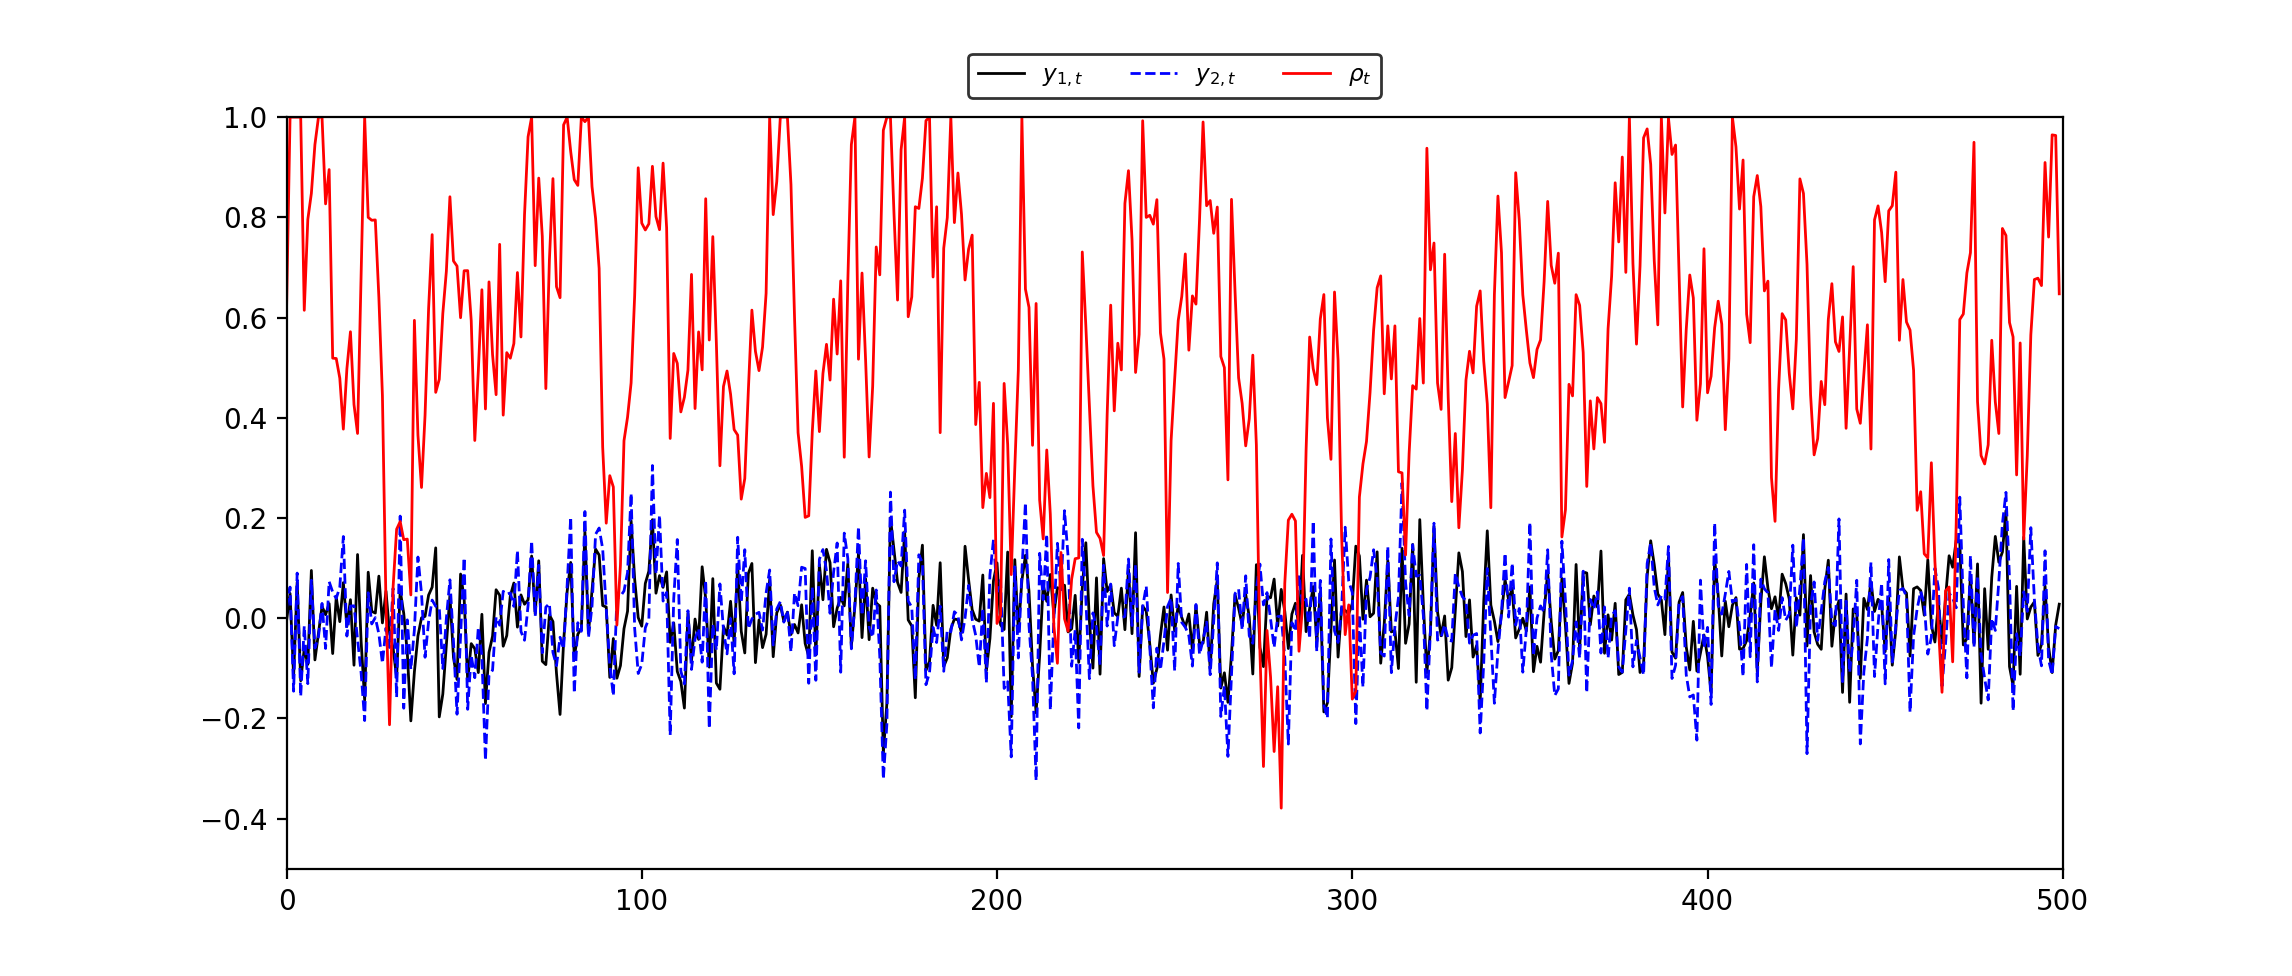
\includegraphics[scale=0.6]{simulation_assetpaths_with_stochastic_correlations.png}
	\caption{Simulated data and time-varying correlations from \eqref{eq:correlation_simulation}.}
	\label{fig:cholesky_simulation}
\end{figure}

\section{Confidence intervals of individual correlation coefficients}
In order to assess some of the statistical properties when (weighted) moving window estimates of correlation coefficients are used as proxies for true correlations as well as for covariates in a learning problem, the estimation uncertainty associated to these coefficients is measured by the width of their $100(1-\eta)\%$ confidence intervals. These confidence intervals were estimated by application of the following bootstrap resampling procedure \citep{ref:Pozzi2012}:

\begin{enumerate}
	\item draw each sample by extracting time units with uniform probability, with replacement;
	\item assign to each selected time unit its corresponding weight, e.g. according to \eqref{eq:pearson_weights} if functional form of weights follow the exponential function 
	\item re-normalize weights to one.
\end{enumerate}

\noindent
For all times $t = \{\Delta t, \Delta t +1, \dots, T\}$, for $\Delta t = \{3, 4, 5, 6, 7, 8, 9, 10, 21, 42, 63, 84, 126, 251\}$\footnote{These time units for $\Delta_t$ correspond to three to ten days, one to four months, six months, and one year of market days. Given the information on this discrete set of datapoints, it is possible to analyse MSE behaviour through linear interpolation between of datapoints.}, a $1000$ samples of size $\Delta t$ have been randomly selected\footnote{A thousand samples is a sufficient number of samples to capture the uncertainty around the estimated values.}. For each subsample the (weighted) correlation coefficient is calculated and, subsequently, the width of the $100(1-\eta)\%$  confidence interval is measured for each coefficient. The parameter $\eta$ is set to $0.99$ in this part of the analysis.    \\

\noindent
\textit{Bootstrapping is conceptually simple, but it's not foolproof. The method involves certain assumptions and has certain limitations. STATE the assumptions of the applied procedure.} \\

\noindent
\textit{Also: Depending on the underlying distribution (for example skewed vs symmetric), the estimations can be biased. There are ways to mitigate that, for example via bias corrected and accelerated bootstrap. But often, going beyond percentile bootstrap could be overkill: we are 
interested in the ORDER OF MAGNITUDE of the measure of confidence anyway, not necessarily an exact value. Hence: the applied bootstrapped procedure should suffice in this goal.} \\

\noindent
\textit{Key questions: What do we expect to see? Can we explain what we see in our analysis? What does this mean for 1) Spurious correlations 2) ml algorithms as estimators for time-varying correlations 3) System of correlations?}  \\

\noindent
\textit{Also: We will apply a walk forward validation such that we will retrain our learner model as new data becomes available. Now do we use a Sliding or Expanding window? We need to decide whether the model will be trained on all data it has available or only on the most recent (1000) observations. Its a tough question: shorter windows increase your parameter risk while longer windows increase your model risk. A short data sample increases the chance that your parameter estimates are way off, conditional on your model specification. A longer data sample increases the chance that you are trying to stretch your model to cover more cases than it can accurately represent. If you were certain that the underlying data-generating process was stable, then the more data you have, the better. If not, then maybe not. In our case the data-generating process is stable. This however is not necessarily the case in real financial processes, which will be the focus in multivariate setting. Let's stick with expanding window for now. Especially since Rob Hyndman also  suggests to follow an expanding window procedure.} 



\section{The Bias-Variance decomposition} \label{sec:mse_decompose}
The purpose of this section is to look at the effect of foundational model properties on the generalization error. The generalization error of a model can be defined as its expected prediction error according to some loss function, e.g. squared error loss in regression. Moreover, decomposition of the expected prediction error into bias and variance terms proves to be useful for analysing the generalization error of proposed learning models in the simulation setting of Section \ref{sec:true_correlation} and Section \ref{sec:proxy_correlation}\footnote{This is possible because, in simulation setting, the true function and the noise distribution that generate the data is known. MSE decomposition will give us therefore an abstract way of explaining why our models show certain behaviour under certain parameterizations (and why our models suck/ not suck). In other words, the bias-variance decomposition framework can be used as a tool for diagnosing underfitting and overfitting.}. \\

\noindent
Let us denote the output variable as $Y$ and our covariates as $X$. If one assumes a relationship such that $Y=f(X)+\epsilon$, where the error $\epsilon \sim N(0,\sigma_\epsilon^2)$, an expression can be derived for the expected prediction error of a regression fit $\hat{f}(X)$ at an input point $X = x_0$, using squared error loss \citep{ref:Hastie2009}:

\begin{align} \label{eq:mse_decomposition_general}
	\text{Err}(x_0) &= E[(Y - \hat{f}(x_0))^2 | X = x_0]\nonumber \\
		      &= \sigma_\epsilon^2 + [E\hat{f}(x_0) - f(x_0)]^2 + E[\hat{f}(x_0)-E\hat{f}(x_0)]^2 \nonumber \\ 
		      &= \sigma_\epsilon^2 + \text{Bias}^2(\hat{f}(x_0)) + \text{Var}(\hat{f}(x_0))\nonumber \\
		      &= \text{Irreducible Error} + \text{Bias}^2 + \text{Variance}. 	
\intertext{The first term in \eqref{eq:mse_decomposition_general} is defined as the variance of the output around its true mean $f(x_0)$, and cannot be mitigated regardless of how accurate $f(x_0)$ is estimated, unless $\sigma_\epsilon^2 = 0$. Moreover, it is independent of both the learning model and the training set and provides a a theoretical lower bound of the generalization error for any model \citep{ref:Louppe2014}. The second term, squared bias, is defined as the amount by which the average of the estimate differs from the true relationship between the covariates and output variable, i.e. the true mean $f(x_0)$. Lastly, the variance is defined as the expected squared deviation of an estimate $\hat{f}(x_0)$ around its mean estimate. Typically, the more complex model $\hat{f}$ is defined, the lower the (squared) bias but the higher the variance. Conversely, as the model complexity is decreased, the (squared) bias tends to increase and the variance tends to decrease. This behaviour is known as the \textit{bias-variance tradeoff}.} 
\intertext{One may estimate a model $\hat{f}(X)$ using any modeling technique and the expected prediction error of a k-nearest neighbor regression fit $\hat{f}_k(X)$ at an input point $X = x_0$ can hence be decomposed:}
	\text{Err}_k(x_0) &= E[(Y - \hat{f}_k(x_0))^2 | X = x_0]\nonumber \\
		      &= \sigma_\epsilon^2 + \text{Bias}^2(\hat{f}_k(x_0)) + \text{Var}(\hat{f}_k(x_0))\nonumber \\
		      &= \sigma_\epsilon^2 + [f(x_0) - \frac{1}{k} \sum_{l=1}^{k}f(x_{(l)})]^2 + \frac{\sigma_\epsilon^2}{k}.  \label{eq:mse_decomposition_knn}
\end{align}

\noindent
where the subscripts $(l)$ in \eqref{eq:mse_decomposition_knn} denote the instances in the set of nearest neighbors to $x_0$. \\

\noindent
The second and third terms in expression \eqref{eq:mse_decomposition_knn} are the (squared) bias and variance components, respectively, and under one's control. For k-nearest neighbors, the model complexity is inversely related to and controlled by the number of neighbors $k$, i.e. the higher the value of $k$, the lower the model complexity. As such, the (squared) bias tends to increase with an increase in $k$, whereas the variance term decreases as the inverse of $k$, i.e. bias-variance tradeoff with variation of $k$.  \\

\noindent
The accuracy of random forests depends on the strength of the individual random forest trees and of the dependence between them \citep{ref:Breiman2001}. A brief discussion of the interplay between these two gives a more formal foundation for understanding the workings of random forests and, inherently, the results obtained from different parameterizations during the simulation study in Sections \ref{sec:true_correlation}-\ref{sec:proxy_correlation}. The expected prediction error of a random forest regression fit $\hat{f}_{rf}(X)$ at an input point $X = x_0$ can be decomposed:

\begin{align}
	\text{Err}_{rf}^B(x_0) &= E[(Y - \hat{f}_{rf}^B(x_0))^2 | X = x_0]\nonumber \\
		&= \sigma_\epsilon^2 + \text{Bias}^2(\hat{f}_{rf}^B(x_0)) + \text{Var}(\hat{f}_{rf}^B(x_0))   \label{eq:mse_decompostion_rf}
\end{align}

\noindent
where $\hat{f}_{rf}^B(x_0) = \frac{1}{B} \sum_{b=1}^B T(x_0;\Theta_b)$, $\{T(x_0; \Theta_b\}_{b=1}^B$ denotes the set of random forest trees and $\Theta_b$ characterizes the $b$th random forest tree. \\

\noindent
From \eqref{eq:mse_decompostion_rf} it is observed that the random forest estimator is constructed by averaging over $B$ random forest trees contained in the set $\{T(x_0; \Theta_b\}_{b=1}^B$. \\       

\noindent
- \textbf{Here only mention implications for decomposing the MSE into bias and variance terms of an ensemble method such as random forest.}  \\   

\noindent
"... since each tree generated in bagging is identically distributed (i.d.), the expectation of an average of B such trees is the same as the expectation of any one of them..." \citep{ref:Hastie2009}. This implies that the bias of a random forest is equal to the bias of any sampled individual tree that is grown to randomly sampled training data $Z$, i.e. $T(x_0; \Theta_b(Z))$: 

\begin{align}
	\text{Bias}(x_0) &= f(x_0) - E_Z\hat{f}_{rf}(x_0) \nonumber \\
		&= f(x_0) - E_ZE_{\Theta|Z}T(x_0;\Theta(Z)) \nonumber \\
		&= f(x_0) - \frac{1}{B} \sum_{b=1}^{B} T(x_0; \Theta_b(Z))
\end{align}

\noindent
"... the only hope of improvement is through variance reduction. An average of $B$ i.i.d. random variables, each with variance $\sigma^2$, has variance  $\frac{\sigma^2}{B}$. If the variables are simply i.d. (identically distributed, but not necessarily independent) with positive pairwise correlation $\rho$, the variance of the average is..." \citep{ref:Hastie2009}:

\begin{align} \label{eq:variance_rf}
	\text{Var}(x_0) &= \rho(x_0)\sigma^2(x_0) + \frac{1-\rho(x_0)}{B}\sigma^2(x_0)	
\end{align} 

\noindent
where $\rho(x_0)$ denotes the Pearson sampling correlation between the predictions of any pair of random forest trees built on the same randomly sampled training dataset. In other words: it is the ratio between the variance due to the randomly sampled training dataset and the total variance, which accounts for randomization due to both the randomly sampled training dataset and the random perturbations from covariate subsampling. $\rho(x_0)$ is always nonnegative and mostly due to the random sampling of the training dataset if $\rho(x_0) \rightarrow 1$. If $\rho(x_0) \rightarrow 0$, variance is mostly due to random perturbations. The sampling variance of any single randomly drawn tree is denoted by $\sigma^2(x_0)$.  \\

\noindent
From \eqref{eq:variance_rf} it is observed that as the number of trees in the random forest estimator gets arbitrarily large, i.e. as $B \rightarrow \infty$, the variance reduces to $\rho(x_0)\sigma^2(x_0)$. Consequently, the variance of a random forest is strictly smaller than the variance of individual trees under the assumption that predictions of individual trees are not perfectly positive correlated, i.e. $\rho < 1$. As to improve on the variance reduction of bagging, correlation $\rho$ has to be minimized without increasing the bias too much, i.e. maintaining strength \citep{ref:Breiman2001}. This is achieved by randomly selecting covariates in the construction of individual trees. The more covariates used, the lower the generalization error of individual trees, i.e. lower bias, but the higher $\rho$, which results in higher variance. Conversely, the statement also holds. There exists a tradeoff between minimizing bias and minimizing variance, i.e. bias-variance tradeoff. \\

\noindent
In summary, the expected prediction error of a random forest regression fit $\hat{f}_{rf}(X)$ at an input point $X = x_0$ decomposes as:

\begin{align}
	\text{Err}_{rf}(x_0) &= E[(Y - \hat{f}_{rf}(x_0))^2 | X = x_0] \nonumber \\
		&=  \sigma_\epsilon^2 + \text{Bias}^2(\hat{f}_{rf}(x_0)) + \text{Var}(\hat{f}_{rf}(x_0)) \nonumber \\ 
		&=\sigma_{\epsilon}^2 + [f(x_0) - E_ZE_{\Theta|Z}T(x_0;\Theta(Z))]^2 + [\rho(x_0)\sigma^2(x_0) + \frac{1-\rho(x_0)}{B}\sigma^2(x_0)]	 
\end{align}
 


\section{KNN, RF Application with True Correlations for Output Variable and Proxies for Covariates} \label{sec:true_correlation}
"In this section, the input variables of the learning models are approximations of actual (unobserved) correlation. Simulation experiments are used to study the effect using approximations of correlations as the input variables on the learner model results, isolating this effect from the approximations of the output variable, which is illustrated in Section \ref{sec:proxy_correlation}. The simulation study will give insight into the (function) approximation capability of KNN/ RF, particularly in comparison to Pearson/ Kendall approximation.  This will give us some initial information wrt possible success of these algorithms in the task of modelling time-varying correlation." \\


\noindent
The accuracy of Pearson and Kendall estimates for time-varying correlation is compared by using mean squared error (MSE) between estimated and actual correlations. The variance of mean squared errors from Pearson estimates in Fig. \ref{fig:mse_pearson_kendall_bootstrap} is approximately 1.78e-3 while that of Kendall is approximately 1.59e-3, i.e. Kendall estimates are slightly less sensitive to the choice of window length compared to Pearson estimates but the difference seems negligible small or might even not be significant. Interestingly, it is observed that Kendall estimates for time-varying correlation have slightly higher MSE values for larger window lengths. A possible explanation for this observation is that the simulated asset returns follow a multivariate normal distribution, i.e. an elliptical distribution. Therefore, it makes sense that a linear correlation coefficient such as Pearson results in lower MSE values for most window lengths. Pearson can get unreliable in the presence of fat-tailed distributions, which is generally a property of real asset return data \citep{ref:Pozzi2012}. It will be interesting to verify whether Kendall is a better choice for approximation of true correlation in the case of real asset return data in Chapter \ref{chap:multivariate_analysis}.  


\begin{figure}[H]
	\centering
	\begin{subfigure}[b]{0.49 \textwidth}
		\centering 
		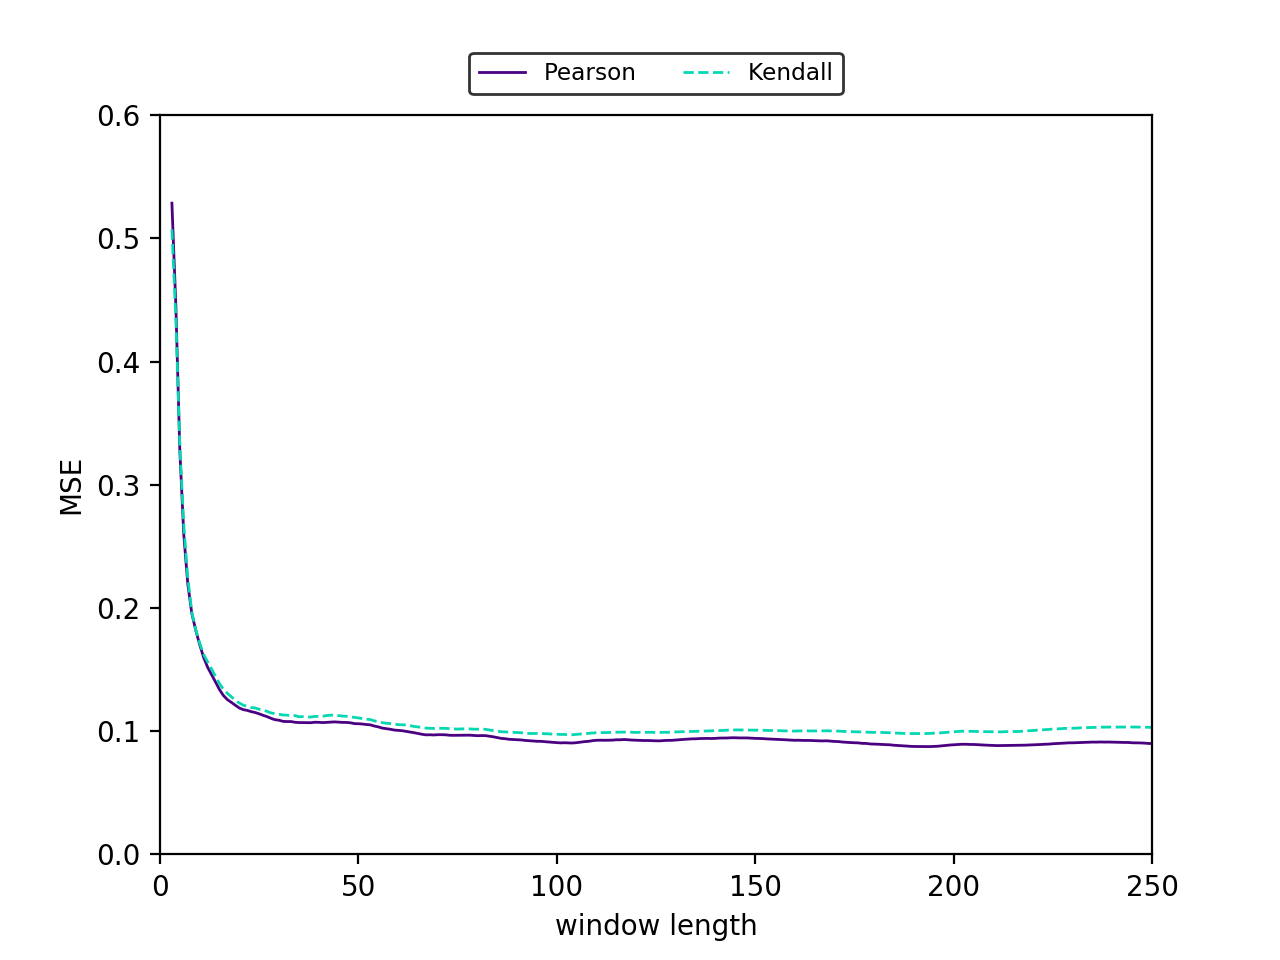
\includegraphics[width=\textwidth]{mse_pearson_kendall.png} 
	\end{subfigure}
	\caption{Comparison MSE for Pearson and Kendall Moving Window bootstrap estimates\protect\footnotemark.}
	\label{fig:mse_pearson_kendall_bootstrap}
\end{figure}

\footnotetext{For Pearson and Kendall correlation approximation using moving window estimates with window sizes 3 through 7 several bootstrapped samples return a standard deviation of zero. This results into NaN values for the associated estimated correlation coefficient as the covariance is divided by zero. These NaN values are excluded for calculation of the mean estimate of Pearson and Kendall correlation coefficient over the test set. Thus, as a result of a smaller number of bootstrapped samples used, estimation of Pearson and Kendall correlation coefficient using moving windows with small window sizes are less robust.} 


\noindent
Fig. \ref{fig:pearson21_bootstrap} and Fig. \ref{fig:kendall21_bootstrap} show that both Pearson moving window estimates and Kendall moving window estimates of correlation change substantially over time indicating the capture of changing correlation levels. Additionally, it is observed that the obtained 99\% confidence intervals around these estimates are rather wide, covering all values in the range $[-1,1]$, which imply that the uncertainty around the estimated values are high \citep{ref:Basturk2016}. \\

\noindent
\textbf{Say something on difference between smoothness/ peaks Pearson/Kendall estimates?} \\  


\begin{figure}[H]  % [h] parameter makes sure figures are located at 'this' location.
	\centering
	\begin{subfigure}[b]{0.49 \textwidth} % sum of widths should be less than text width if all one the same line
		\centering 
		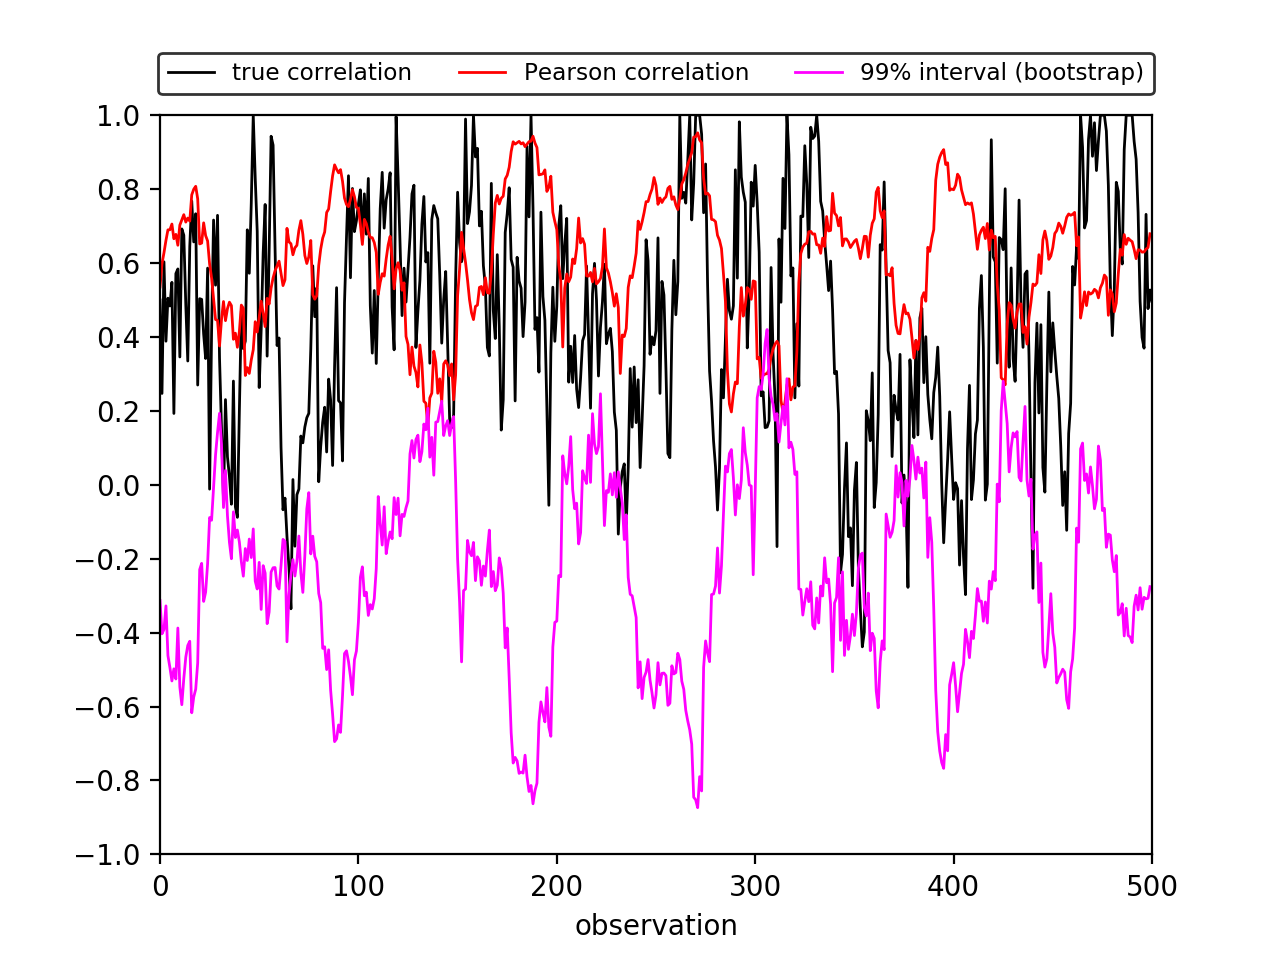
\includegraphics[width=\textwidth]{pearson_21_estimates_bootstrap.png} 
		\caption{Pearson estimates with window size 21.} 		
		\label{fig:pearson21_bootstrap}
	\end{subfigure} 
	\hfill
	\begin{subfigure}[b]{0.49 \textwidth}
		\centering 
		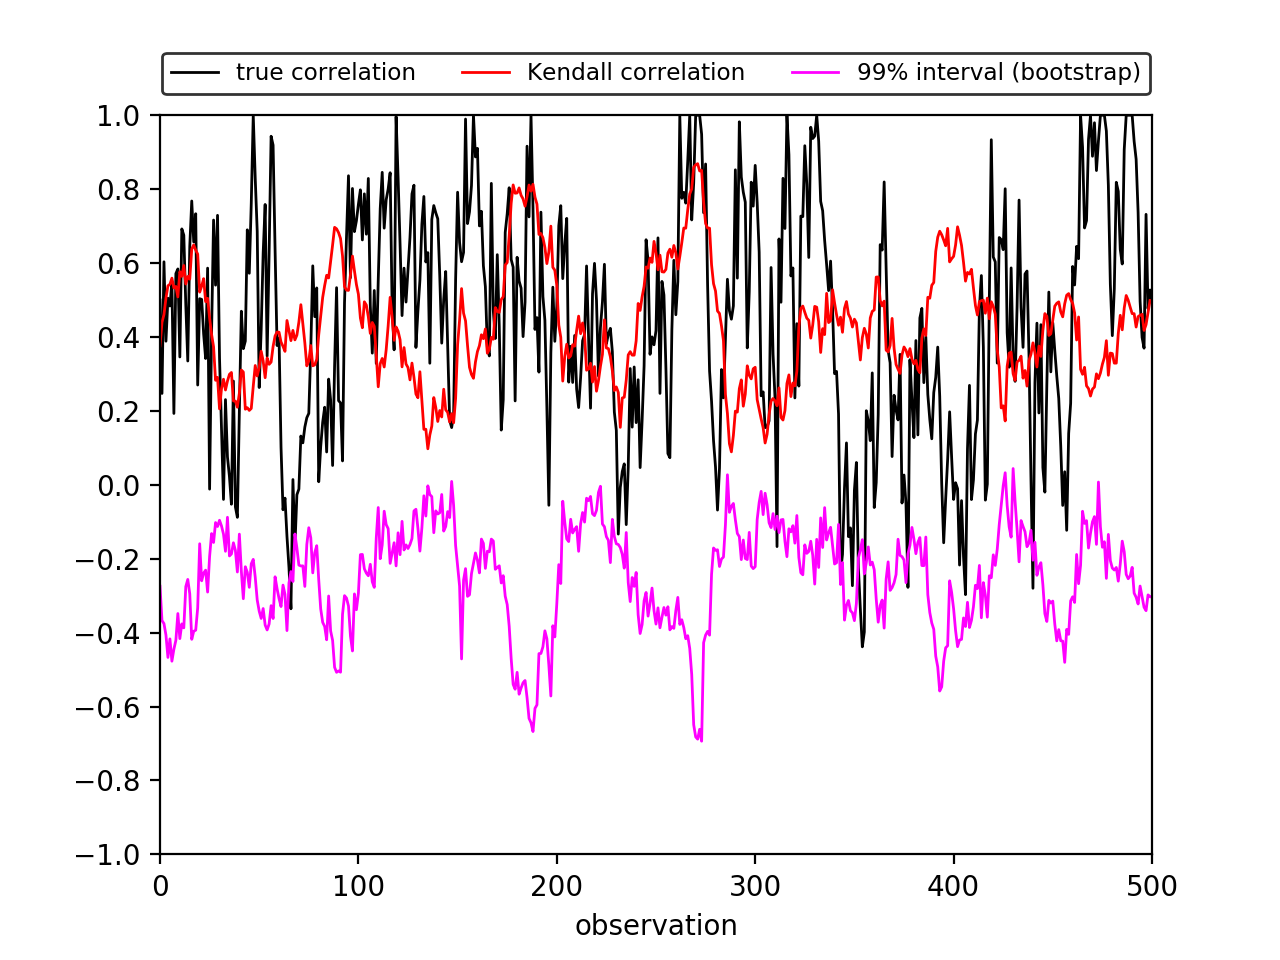
\includegraphics[width=\textwidth]{kendall_21_estimates_bootstrap.png} 
		\caption{Kendall estimates with window size 21.} 		
		\label{fig:kendall21_bootstrap}
	\end{subfigure}
	\hfill
	\begin{subfigure}[b]{0.49 \textwidth} 
		\centering
		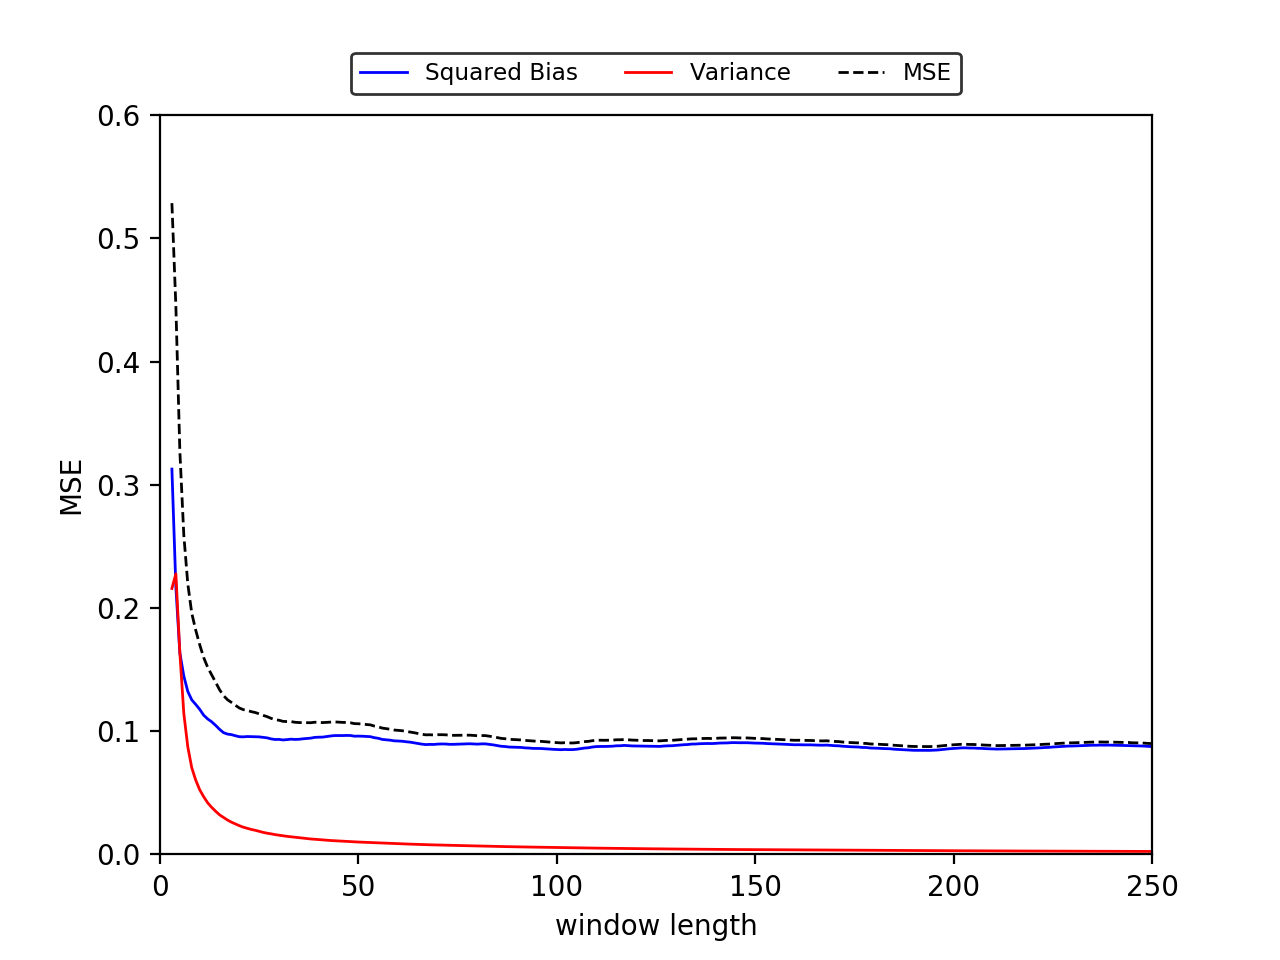
\includegraphics[width=\textwidth]{decom_mse_pearson.png}
		\caption{Bias-variance decomposition for Pearson estimates.}
		\label{fig:decom_mse_pearson}
	\end{subfigure}
	\hfill
	\begin{subfigure}[b]{0.49 \textwidth} 
		\centering
		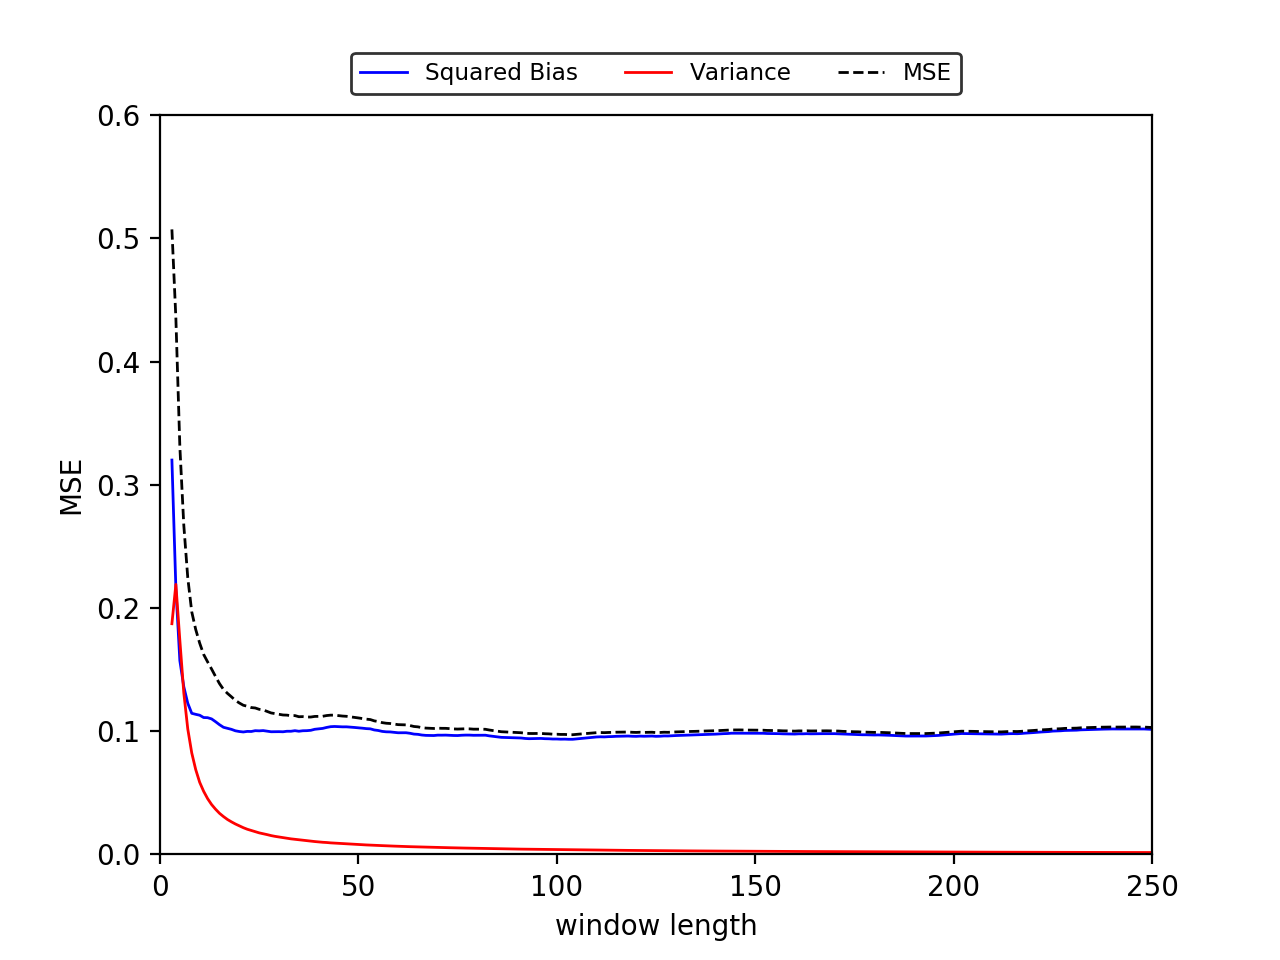
\includegraphics[width=\textwidth]{decom_mse_kendall.png}
		\caption{Bias-variance decomposition for Kendall estimates.}
		\label{fig:decom_mse_kendall}
	\end{subfigure}
	\caption{MSE for Pearson and Kendall Moving Window bootstrap estimates.}
	\label{fig:decom_mse_pearson_kendall_true}
\end{figure}

\noindent
Moreover, Pearson and Kendall estimates are very sensitive to the choice of the window length used for correlation estimates. This is illustrated by the bias-variance decomposition of the mean squared error (MSE) between estimated and actual correlations, shown in Fig. \ref{fig:decom_mse_pearson} and Fig. \ref{fig:decom_mse_kendall}. One can observe an inverse relationship between the choice of window length (i.e. the bootstrap sample size) and value of the variance term in the MSE decomposition. This is explained by the fact that as the bootstrap sample size increases with an increase of the window length, the standard error (i.e. the standard deviation of the sampling distribution) decreases. In other words, as the bootstrap sample size increases, the variability of sampling distribution decreases which would show through smaller 99\% confidence intervals. In these figures it is shown through a decrease in de variance term of the bias-variance decomposition of the mean squared error (MSE) between estimated and actual correlations. \\

\noindent
Concluding, Pearson and Kendall moving window estimates of time-varying correlation satisfy the positive semi-definiteness condition in the time-varying correlation matrix $R_t$ for all time $t$ under all choices of window length. Fig. \ref{fig:det_pearson_kendall} presents the obtained minimum determinants of $R_t$ for all choices of window length. In fact, \cite{ref:Pozzi2012} give proves that Pearson and Kendall correlation matrices generally are positive semi-definite matrices.     

\begin{figure}[H]
	\centering
	\begin{subfigure}[b]{0.49 \textwidth}
		\centering 
		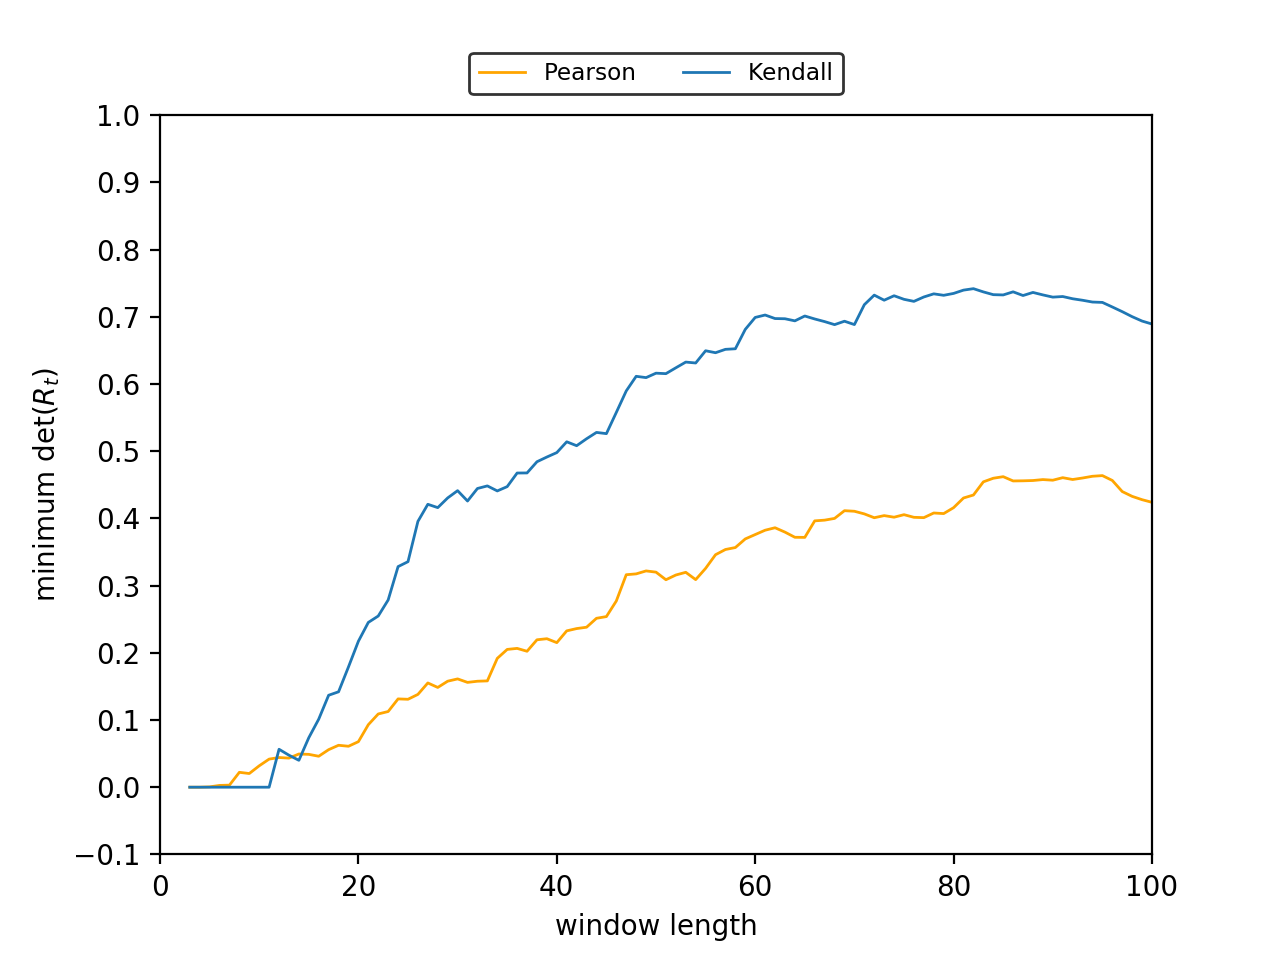
\includegraphics[width=\textwidth]{det_pearson_kendall} 
	\end{subfigure}
	\caption{Minimum det($R_t$) from Pearson and Kendall Moving Window bootstrap estimates.}
	\label{fig:det_pearson_kendall}
\end{figure}





%%%%%% NEAREST neighbor TRUE COR %%%%%%%%
\subsection{Nearest neighbor} \label{sec:knn_true_cor}
In order to obtain time-varying correlations, $\rho_t$, with k-nearest multivariate neighbor algorithm, the set of covariates is defined by lagged Pearson and Kendall moving window estimates and minimum and maximum asset return values in the last period, denoted by $min_{i,j}(y_{i,j,t-1})$, and $max_{i,j}(y_{i,j,t-1})$, respectively.  \\

\noindent
The accuracy of KNN estimates with Pearson and Kendall covariates for time-varying correlation is compared by using mean squared error (MSE) between estimated and actual correlations. MSE from KNN with Pearson and Kendall moving window estimates of correlation for covariates are shown in Fig. \ref{fig:mse_knn5_pearson_kendall_true}. Regardless of the choice of window length, MSE from KNN with Pearson and Kendall covariates are between 0.0939 and 0.1071, and 0.0929 and 0.1071, respectively. The variance of MSE from KNN estimates with Pearson covariates is approximately 6.07e-6 while that of KNN estimates with Kendall covariates is approximately 5.66e-6. KNN thus appears to be insensitive to the choice of window length, regardless whether the set of covariates is constructed from Pearson or Kendall moving window estimates of correlation. KNN's property of insensitivity to the choice of window length is preferred over Pearson and Kendall's property of being highly sensitive to the choice of the window length used for correlation estimates as depicted in Fig. \ref{fig:mse_pearson_kendall_bootstrap}.  \\

\noindent
Moreover, KNN estimates of time-varying correlation where the set of covariates is constructed from Pearson and Kendall moving window estimates and true correlation as output variable, satisfy the positive semi-definiteness condition in the time-varying correlation matrix $R_t$ for all time $t$ under all choices of window length. Fig. \ref{fig:det_knn5_pearson_kendall_true} presents the obtained minimum determinants of $R_t$ for all choices of window length.  
     
\begin{figure}[H]
	\centering
	\begin{subfigure}[b]{0.49 \textwidth} 
		\centering
		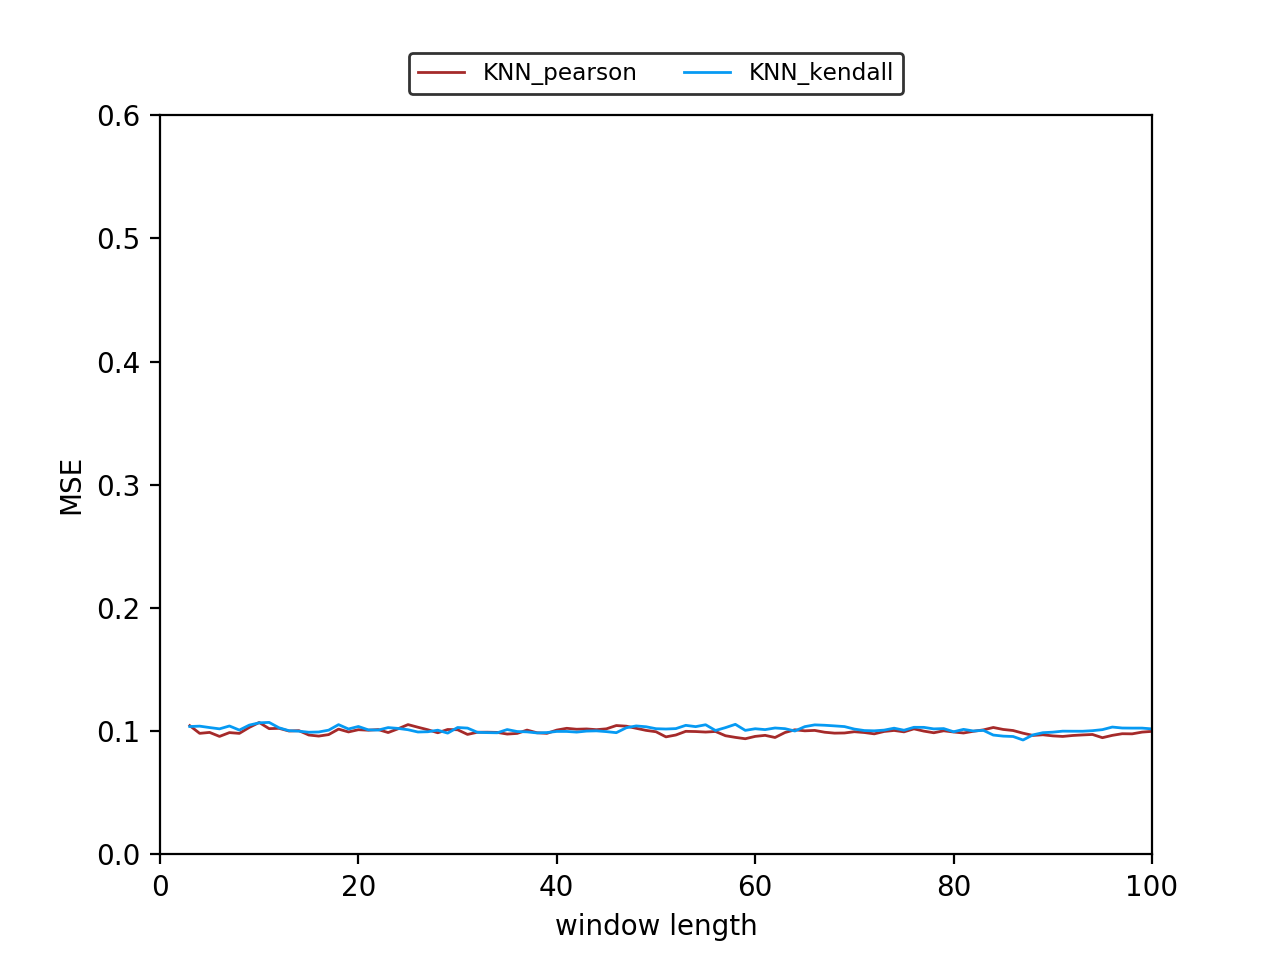
\includegraphics[width=\textwidth]{mse_knn5_pearson_kendall_true.png}
		\caption{MSE for KNN with covariates from Pearson and Kendall and true correlation.}
		\label{fig:mse_knn5_pearson_kendall_true}
	\end{subfigure}
	\hfill
	\begin{subfigure}[b]{0.49 \textwidth} 
		\centering
		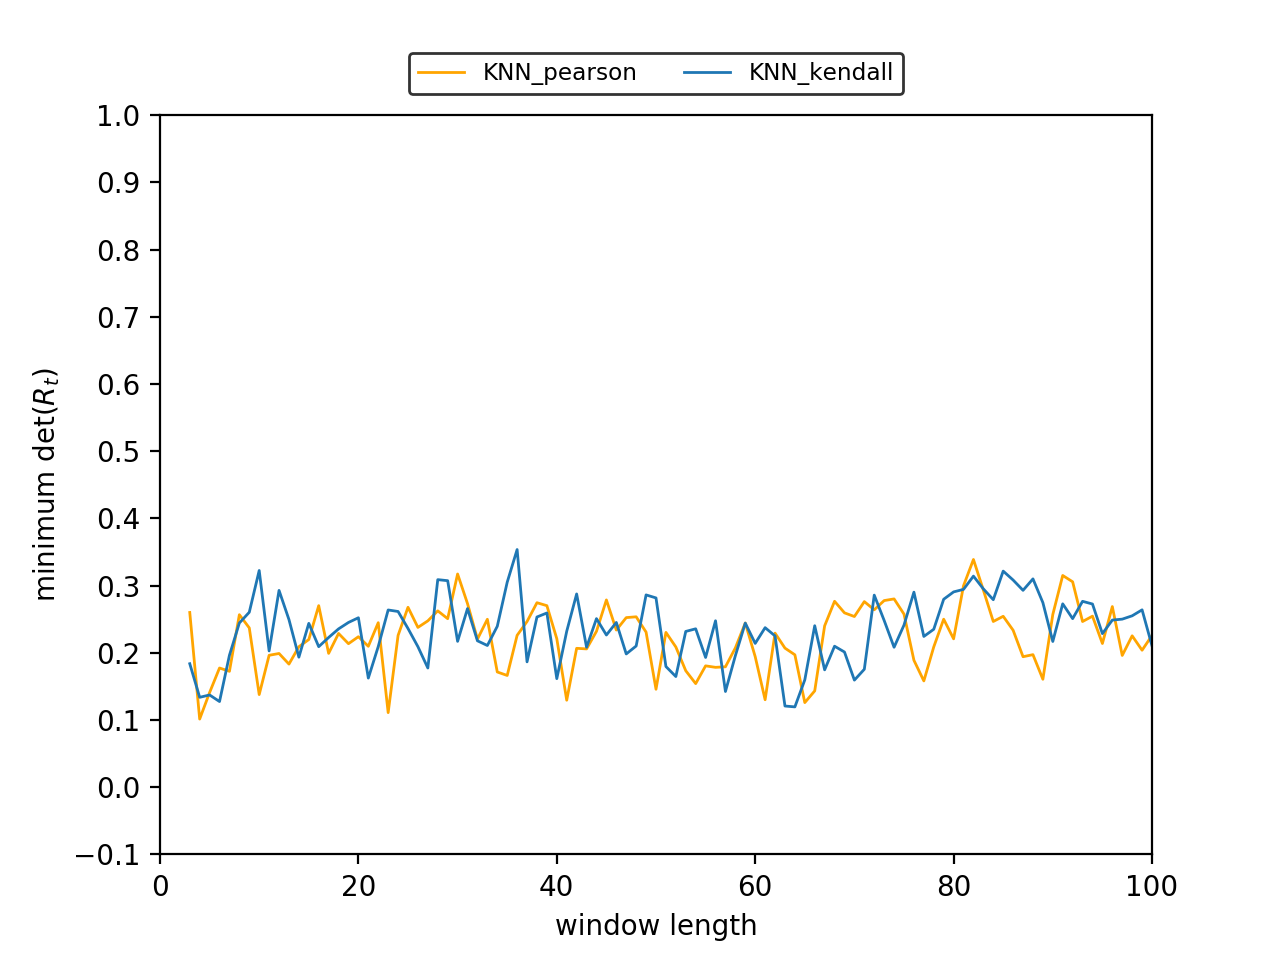
\includegraphics[width=\textwidth]{det_knn5_pearson_kendall_true}
		\caption{Minimum determinants for KNN with covariates from Pearson and Kendall and true correlation.}
		\label{fig:det_knn5_pearson_kendall_true}
	\end{subfigure}
	\caption{Comparison MSE and minimum determinants for KNN(n\_neighbors=5) with covariates from Pearson and Kendall and true correlation.}
	\label{fig:mse_det_knn5_pearson_kendall_true}
\end{figure}



\noindent
From visual inspection of the plots in Fig. \ref{fig:knn_pearson21_bootstrap_true} and Fig. \ref{fig:knn_kendall21_bootstrap_true} it seems that the uncertainty in the time-varying correlation $\rho_t$, which is illustrated by the $99\%$ confidence interval, is smaller for KNN estimates compared to Pearson and Kendall moving window estimates under the same window length of 21. KNN estimates of correlation with number of neighbors equal to 5 are, however, much more volatile. This may be a less desirable result as it is not expected that correlation between assets changes that drastically at each time period. Rather, correlation is expected to vary gradually over time \citep{ref:Basturk2016}. It is observed though that, as with an increase in the choice of window length for Pearson and Kendall moving window estimates of correlation, an increase in the number of neighbors results in smoother KNN estimates of correlation. \\

\noindent
\textbf{Say something on the bias-variance decomposition of knn with pearson and kendall.} \\

\noindent
The MSE decompositions into bias and variance terms from KNN estimates of correlation are shown in Fig. \ref{fig:decom_mse_knn5_pearson_true} and Fig. \ref{fig:decom_mse_knn5_kendall_true}. These figures indicate that the KNN algorithm is considerably less sensitive to the choice of the window length for smaller window sizes when compared to Pearson and Kendall moving window estimates of correlation. The uncertainty around the estimated correlations appears to be marginally affected by the choice of the window length for all window sizes. This statement is supported by the fact that the variance as a function of the window length behaves like a (more or less) constant red line in these figures.   

\begin{figure}[H]  % [h] parameter makes sure figures are located at 'this' location.
	\centering
	\begin{subfigure}[b]{0.49 \textwidth} % sum of widths should be less than text width if all one the same line
		\centering 
		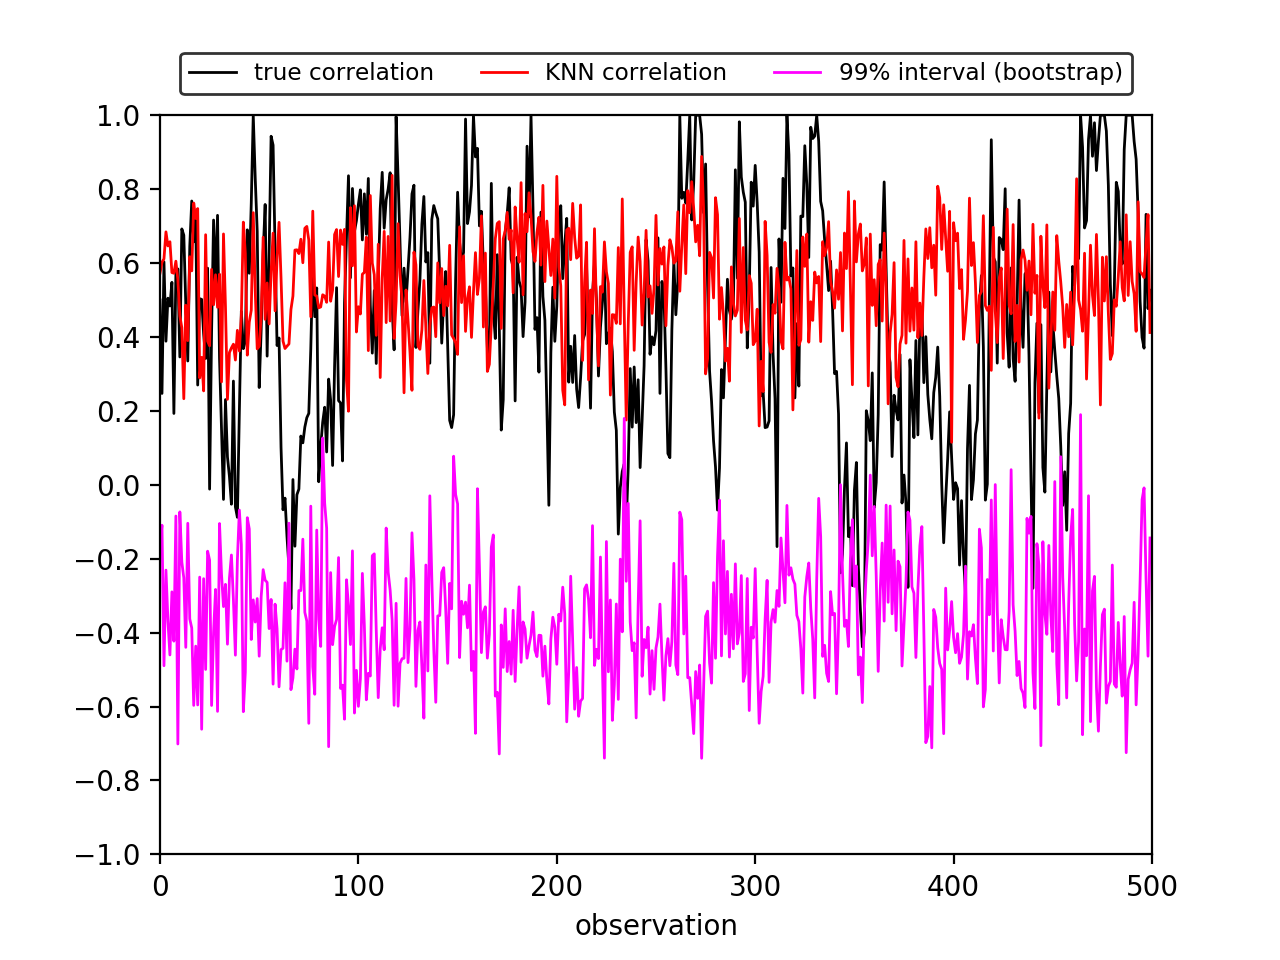
\includegraphics[width=\textwidth]{knn_pearson_21_estimates_bootstrap_true.png} 
		\caption{KNN estimates with window size 21, Pearson as covariate and true correlation.} 	
		\label{fig:knn_pearson21_bootstrap_true}
	\end{subfigure} 
	\hfill	
	\begin{subfigure}[b]{0.49 \textwidth} 
		\centering 
		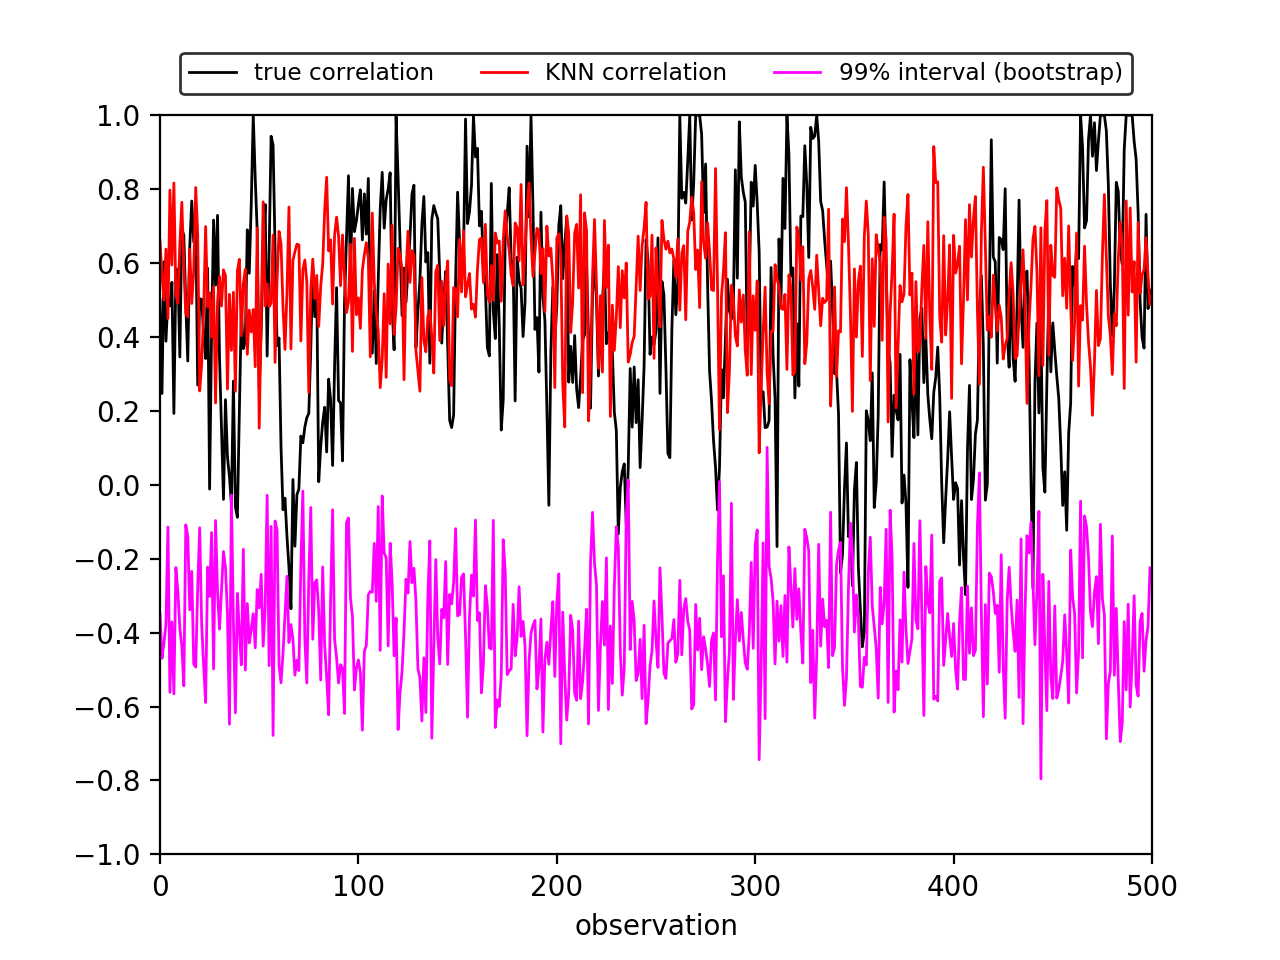
\includegraphics[width=\textwidth]{knn_kendall_21_estimates_bootstrap_true.png} 
		\caption{KNN estimates with window size 21, Kendall as covariate and true correlation.} 
		\label{fig:knn_kendall21_bootstrap_true}
	\end{subfigure} 
	\hfill	
	\begin{subfigure}[b]{0.49 \textwidth}
		\centering 
		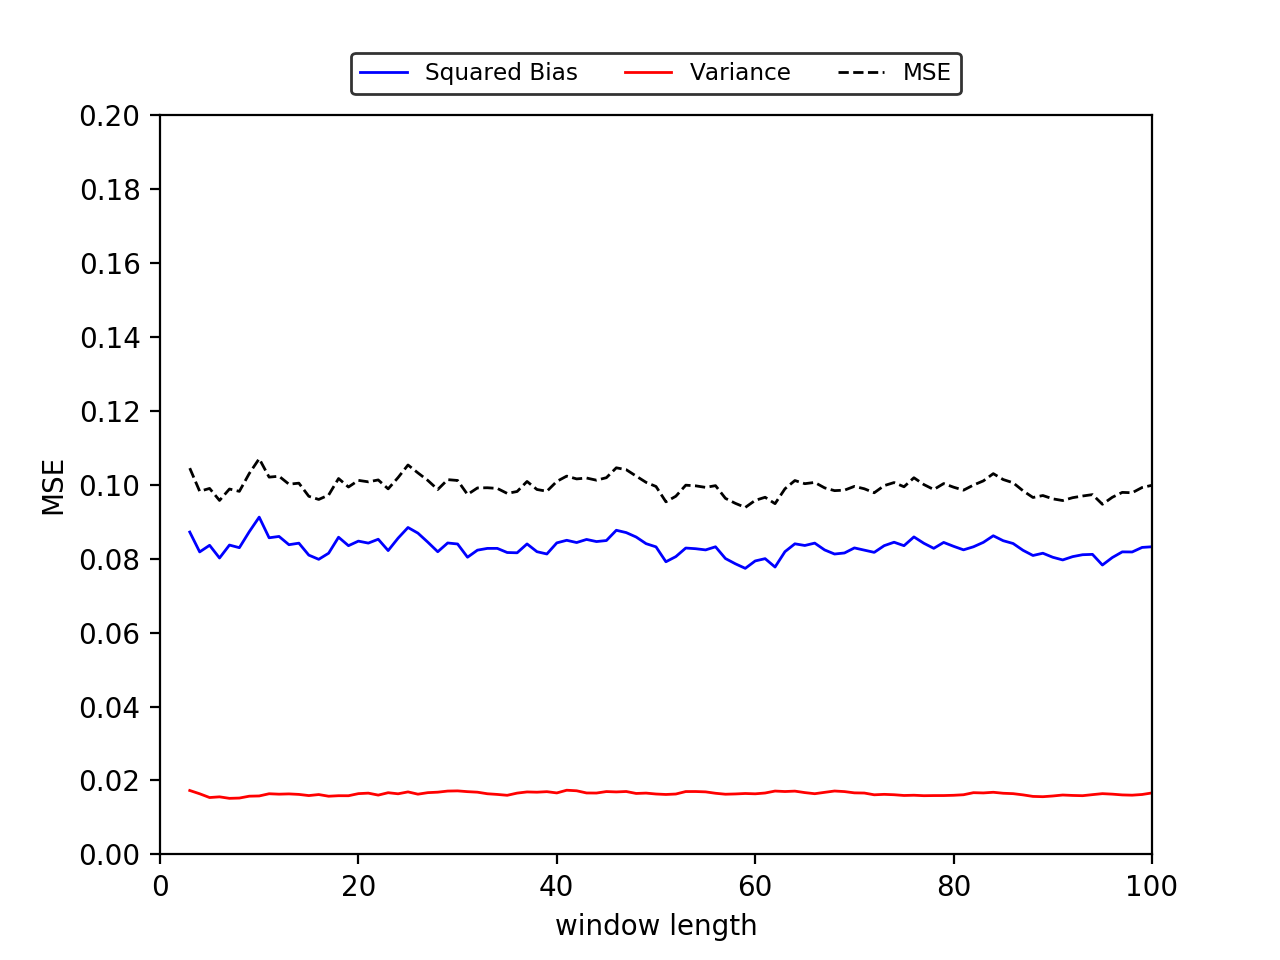
\includegraphics[width=\textwidth]{decom_mse_knn5_pearson_true.png} 
		\caption{Bias-variance decomposition for KNN estimates with Pearson as covariate and true correlation.} 	
		\label{fig:decom_mse_knn5_pearson_true}
	\end{subfigure}
	\hfill  
	\begin{subfigure}[b]{0.49 \textwidth}
		\centering 
		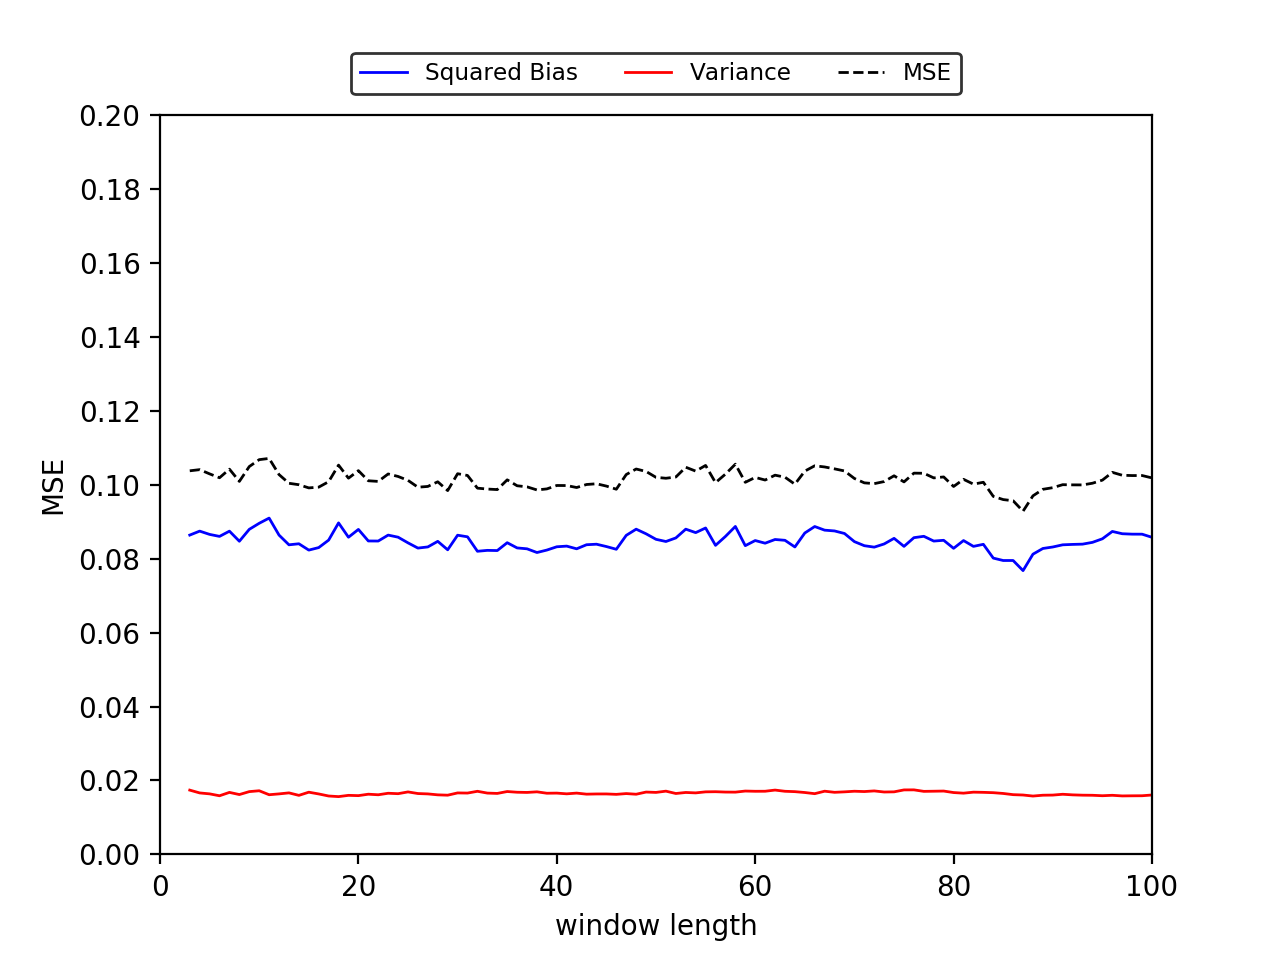
\includegraphics[width=\textwidth]{decom_mse_knn5_kendall_true.png} 
		\caption{Bias-variance decomposition for KNN estimates with Kendall as covariate and true correlation.} 
		\label{fig:decom_mse_knn5_kendall_true}
	\end{subfigure}
	\caption{MSE for KNN estimates with Pearson and Kendall Moving Window bootstrap estimates as covariates and true correlation.}
	\label{fig:decom_mse_knn5_pearson_kendall_true}
\end{figure}


\noindent
Fig. \ref{fig:decom_mse_pearson_kendall_true} depicted an inverse relationship between the choice of the window length and the uncertainty around Pearson and Kendall moving window estimates of correlation. The KNN algorithm has a similar property: Simulation results in Tabel \ref{tab:mse_decomp_knn_pearson_kendall_true} show an inverse relationship between the choice of the number of nearest neighbors used in the estimation of correlations and the uncertainty around the estimated correlations, regardless whether Pearson or Kendall estimates are used for defining the set of covariates. It is clearly observed that an increase in the number of neighbors $k$ results in a decrease of the variance, and conversely. This observation is in line with our discussion on MSE decomposition for the KNN algorithm and Eq. \eqref{eq:mse_decomposition_knn} from Section \ref{sec:mse_decompose}. Additionally, it was stated that the higher the value of $k$, the lower the model complexity and, as such, the squared bias tends to increase with an increase in $k$. However, simulation results depicted in Tabel \ref{tab:mse_decomp_knn_pearson_kendall_true} indicate no increase in squared bias with an increase in $k$ up to $k=800$. The first increase in squared bias is observed when the number of neighbors is approximately 900. For all $k$ smaller than 900 a decrease in squared bias is observed with an increase in $k$. This statement is more clearly shown through a geometrical representation of the MSE decomposition as a function of the number of neighbors for $k \in \{5, 10, 25, 50, 100\}$ in Fig. \ref{fig:knn5_pearson_kendall_sens_analysis_true}. \\  




%% TABLE
\begin{table}[H]
\centering
\captionsetup[subtable]{position=below}
%\captionsetup[table]{position=below}
\begin{subtable}{0.49\linewidth}
\centering
\begin{tabular}{r  c  c  c} 
\toprule
\multicolumn{1}{ r }{\textbf{k}} &
\multicolumn{1}{ c }{\textbf{Squared Bias}} &
\multicolumn{1}{ c }{\textbf{Variance}} &
\multicolumn{1}{ c }{\textbf{MSE}} \\
\midrule 

5                                     & 0.0913                         & 0.0158                & 0.1071     \\
10                                   & 0.0831                         & 0.0087                & 0.0917     \\
25                                   & 0.0785 	                    & 0.0037                & 0.0821     \\
50                                   & 0.0781                         & 0.0018                & 0.0799     \\
100                                 & 0.0785                         & 9.23e-4               & 0.0794      \\
200                                 & 0.0776                         & 4.62e-4               & 0.0781      \\
400                                 & 0.0768                         & 2.31e-4               & 0.0770      \\
600                                 & 0.0757                         & 1.55e-4               & 0.0759     \\
800                                 & 0.0756                         & 1.18e-4               & 0.0757      \\
900				     & 0.0761			   & 1.06e-4              & 0.0760      \\
1000                               & 0.0767                         &  9.70e-5              & 0.0768     \\ [1ex]
\bottomrule
\end{tabular}
\caption{MSE for KNN estimates with window size 10, Pearson as covariate and true correlation.}
\label{tab:mse_decomp_knn_pearson_true}
\end{subtable}
\hfill
\begin{subtable}{0.49\linewidth}
\centering
\begin{tabular}{r  c  c  c} 
\toprule
\multicolumn{1}{ r }{\textbf{k}} &
\multicolumn{1}{ c }{\textbf{Squared Bias}} &
\multicolumn{1}{ c }{\textbf{Variance}} &
\multicolumn{1}{ c }{\textbf{MSE}} \\
\midrule 

5                                     & 0.0896                         &  0.0172               & 0.1068   \\
10                                   & 0.0828                         & 0.0092                & 0.0920   \\
25                                   & 0.0764	                   & 0.0038                & 0.0802    \\
50                                   &  0.0749                        & 0.0019               & 0.0769    \\
100                                 & 0.0749                         & 9.47e-4               & 0.0759    \\
200                                 &  0.0753                        & 4.69e-4              & 0.0757    \\
400                                 &  0.0750                        & 2.37e-4              & 0.0752    \\
600                                 & 0.0749                         & 1.59e-4             & 0.0750     \\
800                                 &   0.0750                       & 1.21e-4             & 0.0751     \\
900				     &  0.0757			   & 1.08e-4             & 0.0758     \\
1000                               &  0.0763                        & 9.80e-5             & 0.0764     \\  [1ex]
\bottomrule
\end{tabular}
\caption{MSE for KNN estimates with window size 10, Kendall as covariate and true correlation.}
\label{tab:mse_decomp_knn_kendall_true}
\end{subtable}
\caption{Mean Squared Error (MSE) decomposition as a function of the number of neighbors (k) for KNN with proxy for covariates and true correlation.}
\label{tab:mse_decomp_knn_pearson_kendall_true}
\end{table}

\noindent
Fig. \ref{fig:knn5_pearson_sens_analysis_true} and Fig. \ref{fig:knn5_kendall_sens_analysis_true}  depict geometrical representations of the simulation results for KNN estimates with Pearson and Kendall covariates (and true correlation), respectively. The MSE decomposition as a function of the number of neighbors for $k \in \{5, 10, 25, 50, 100\}$ clearly shows a decrease in the squared bias with an increase in $k$. Given
Eq. \eqref{eq:mse_decomposition_knn} and our discussion from Section \ref{sec:mse_decompose} one might have expected an increase in squared bias with an increase in $k$. A possible explanation for the behaviour depicted in Fig. \ref{fig:knn5_pearson_kendall_sens_analysis_true} may be that up to some $k$, an increase in $k$ implies additional neighbors containing informational value are used for the estimation of time-varying correlations. Logically, the inclusion of additional neighbors containing informational value results into more accurate estimates of correlation, i.e. a decrease in squared bias. As of some $k$, additional neighbors only add noise to the estimation process which results into increased squared bias.    

\begin{figure}[H]  % [h] parameter makes sure figures are located at 'this' location.
	\centering
	\begin{subfigure}[b]{0.49 \textwidth} % sum of widths should be less than text width if all one the same line
		\centering 
		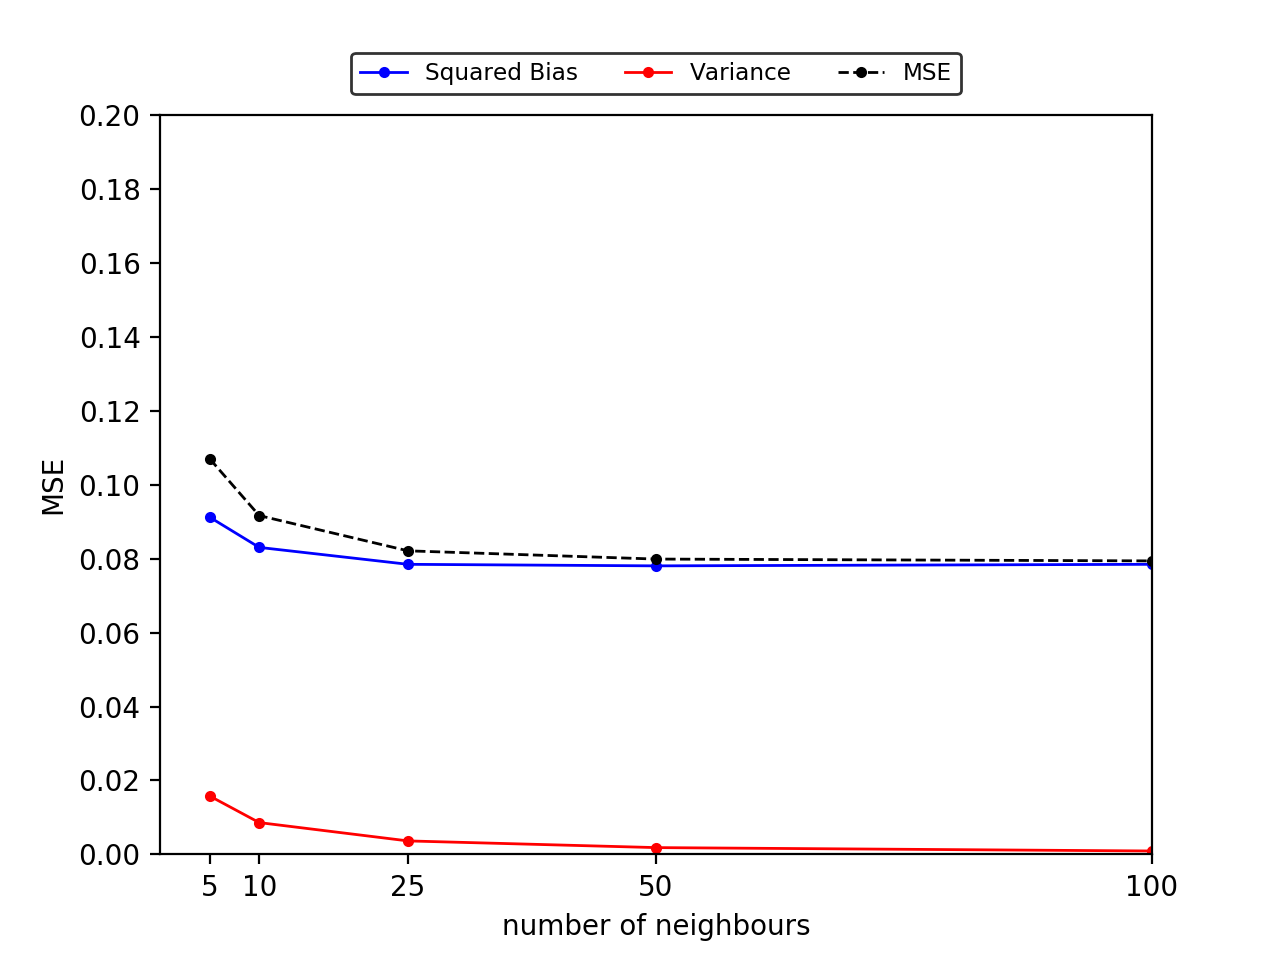
\includegraphics[width=\textwidth]{sens_analysis_mse_knn_pearson_true.png} 
		\caption{KNN estimates with window size 10, Pearson as covariate and true correlation.}
		\label{fig:knn5_pearson_sens_analysis_true}
	\end{subfigure} 
	\hfill	
	\begin{subfigure}[b]{0.49 \textwidth} 
		\centering 
		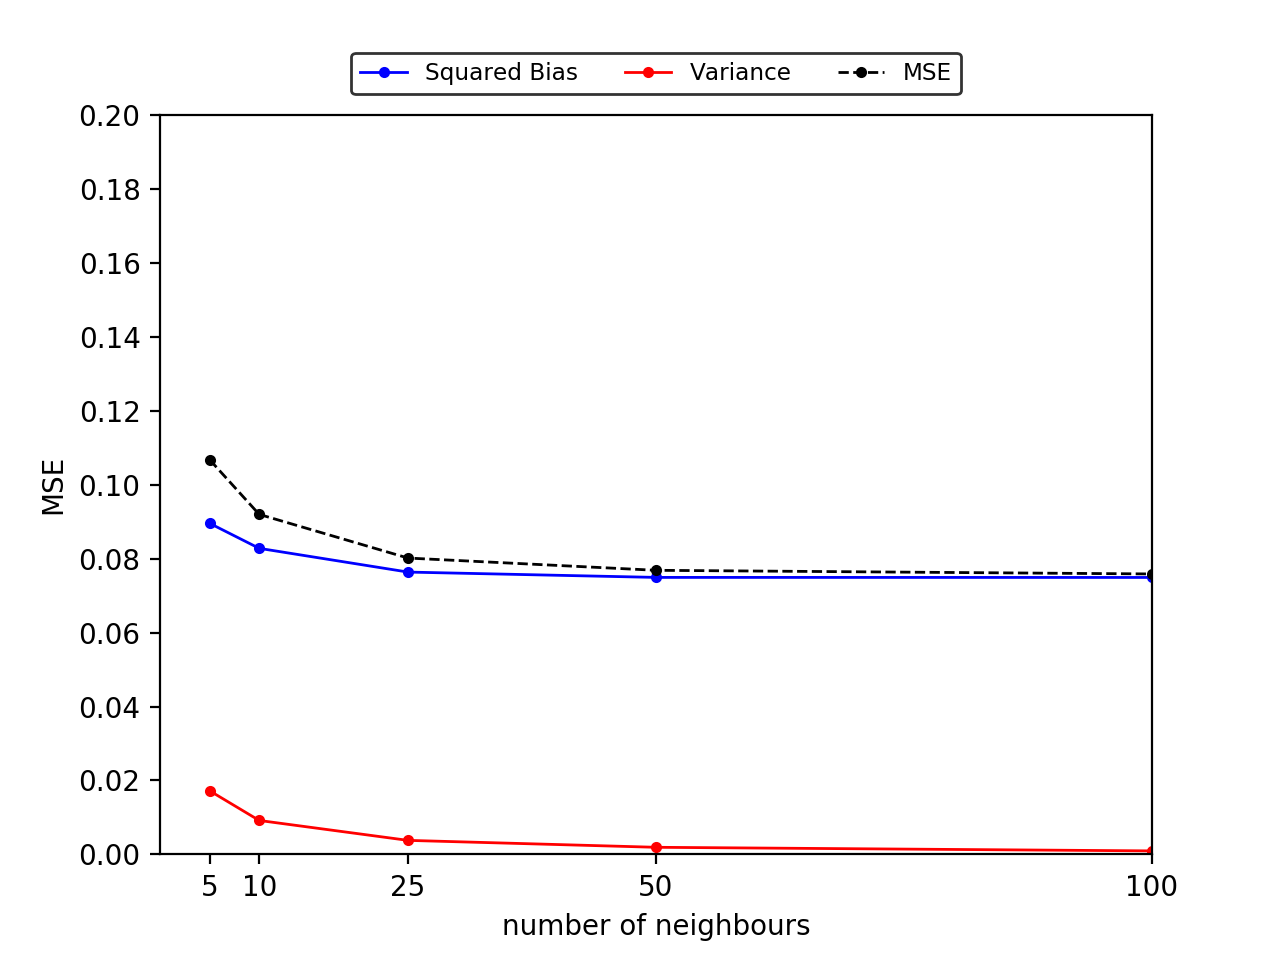
\includegraphics[width=\textwidth]{sens_analysis_mse_knn_kendall_true.png} 
		\caption{KNN estimates window size 10, Kendall as covariate and true correlation.} 
		\label{fig:knn5_kendall_sens_analysis_true}
	\end{subfigure} 
	\caption{MSE as function of number of neighbors for KNN estimates with Pearson and Kendall as covariates and true correlation.}
	\label{fig:knn5_pearson_kendall_sens_analysis_true}
\end{figure}

\noindent
Next, two more interesting parameterisations of the KNN learner model are analysed. In both parameterisations, the set of neighbors used for point estimation of time-varying correlation is defined as the entire training set. However, in the first parameterisation, the KNN algorithm uses an uniformly weighted average of correlations, i.e. each of the neighbors contributing equally to the point estimate of time-varying correlation. In the second parameterisation, the KNN algorithm uses an inverse distance weighted average of correlations, as defined in Eq. \ref{eq:IDWfunction} \citep{ref:Shepard1968}. The MSE decomposition of both parameterisations with Pearson covariates and true correlation is depicted in Fig. \ref{fig:decom_mse_knn_len_train_IDW_pearson_kendall_true}. It is clear that the variance terms becomes negligible small in case the set of neighbors used for point estimation of time-varying correlation is defined as the entire training set, regardless of the weighting function. The red line of the variance is barely observable in the bottom of Fig. \ref{fig:decom_mse_knn_len_train_pearson_true} and Fig. \ref{fig:decom_mse_knn_IDW_pearson_true}. This is in line with results depicted in Tabel \ref{tab:mse_decomp_knn_pearson_kendall_true} where the value of the variance term is negligible small for $k=1000$, regardless whether the set of covariates is constructed from Pearson or Kendall moving window estimates of correlation.          

\begin{figure}[H]  % [h] parameter makes sure figures are located at 'this' location.
	\centering
	\begin{subfigure}[b]{0.49 \textwidth}
		\centering 
		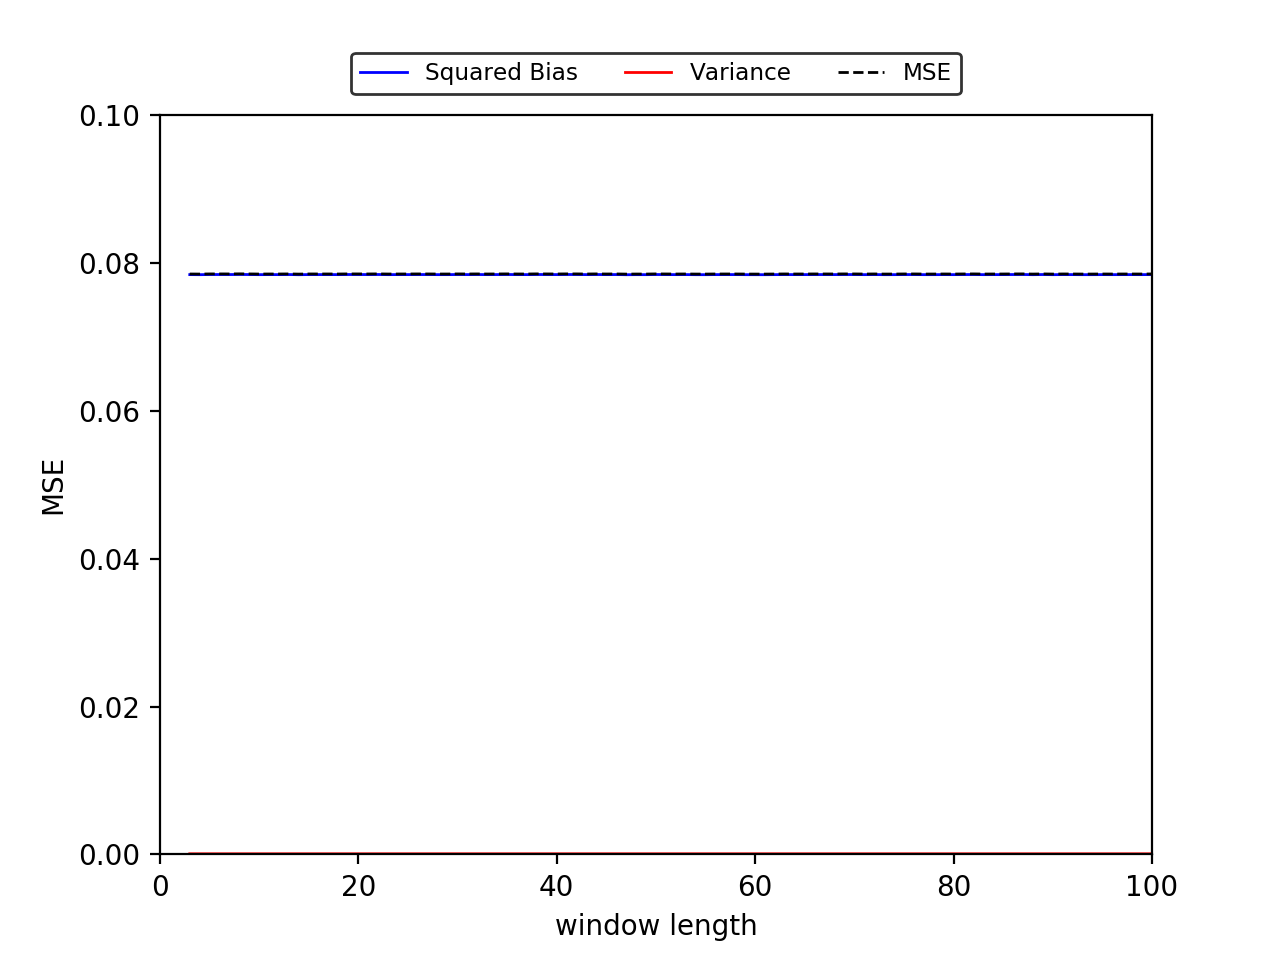
\includegraphics[width=\textwidth]{decom_mse_knn_len_train_pearson_true.png} 
		\caption{Bias-variance decomposition for KNN estimates constructed from uniformly weighted averages.} 	
		\label{fig:decom_mse_knn_len_train_pearson_true}
	\end{subfigure}
	\hfill  
	\begin{subfigure}[b]{0.49 \textwidth}
		\centering 
		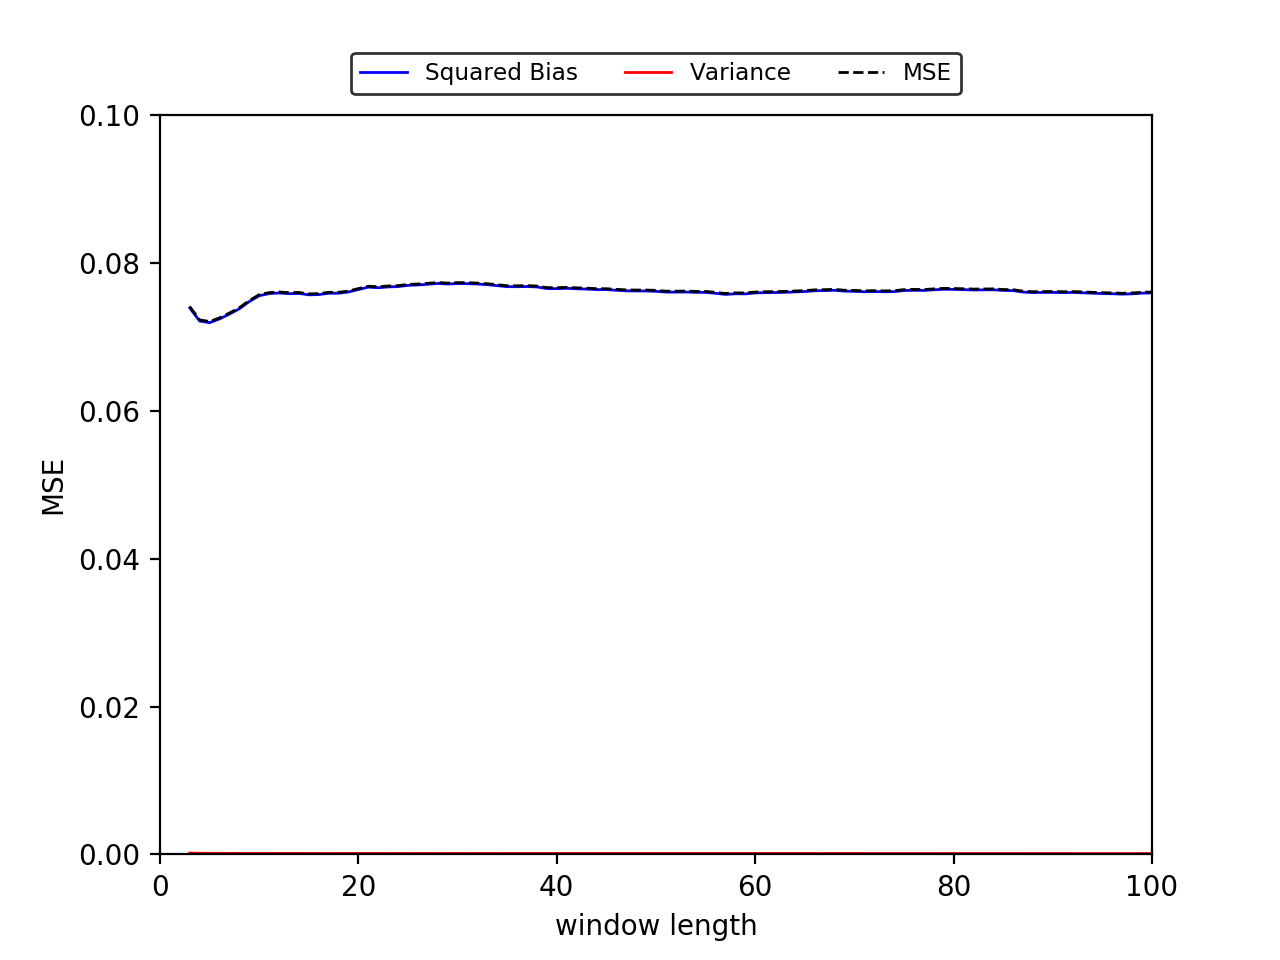
\includegraphics[width=\textwidth]{decom_mse_knn_IDW_pearson_true.png} 
		\caption{Bias-variance decomposition for KNN estimates constructed from inverse distance weighted averages.} 
		\label{fig:decom_mse_knn_IDW_pearson_true}
	\end{subfigure}
	\caption{MSE for KNN estimates with different weighting functions, Pearson Moving Window bootstrap estimates as covariates and true correlation.}
	\label{fig:decom_mse_knn_len_train_IDW_pearson_kendall_true}
\end{figure}

\noindent
The accuracy of the two different parameterisations is compared by using mean squared error (MSE) between estimated and actual correlations. MSE from KNN with an uniform weighting function is approximately 0.0785, regardless of the choice of window length and whether Pearson or Kendall moving window estimates are use for constructing the set of covariates. MSE from KNN with an inverse distance weighting function is approximately between 0.0721 and 0.0774, and between 0.0727 and 0.0771 when Pearson and Kendall moving window estimates are used as covariates, respectively. This implies that slightly lower MSE values are obtained with an inverse distance weighting function as opposed to an uniform weighting function, which is line with our discussion from Section \ref{sec:knn}. It makes sense to have training instances with a higher amount of proximity to the test instance contribute more to the value of the output variable than training instances with a lower amount of proximity to the test instance. Moreover, Fig. \ref{fig:decom_mse_knn_len_train_IDW_pearson_kendall_true} shows that both parameterisations are insensitive to the choice of window length, regardless of the weighting function and choice of covariate. In fact, the variance of MSE from KNN with uniform weighting function and inverse distance weighting function are 5.00e-11 and 8.55e-7, respectively, i.e. hardly significantly different from one another. \\ 

\noindent
This section is concluded with a comparison of the function approximation capabilities of the KNN algorithm and Pearson and Kendall moving window estimates. The comparison is based on MSE between estimated and actual correlations. Fig. \ref{fig:mse_knn5_idw_pearson_kendall_true} shows MSE from KNN with default parameterisation, i.e. number of neighbors equals 5, an alternative parameterisation with an inverse distance weighting function as well as Pearson and Kendall moving window estimates of time-varying correlations. According to MSE, parameterisations of the KNN algorithm where the number of neighbors is 5 or 10 perform better than those of Pearson and Kendall moving window estimates for small window sizes. Moreover, parameterisations of the KNN algorithm with an alternative distance weighting function and where the entire training data set is used for estimating correlation result in significantly smaller MSE compared to Pearson and Kendall moving window estimates for all window sizes. In fact, the simulation study shows that the KNN algorithm outperforms Pearson and Kendall moving window estimates of correlation for all window sizes when the number of neighbors $k \in \{25, 50, 100\}$ in addition to both alternative parameterisations. Finally, the variance of MSE from KNN estimates with default parameterisation and with an inverse distance weighting function in Fig. \ref{fig:mse_knn5_idw_pearson_kendall_true} are 6.07e-6 and 8.55e-7, respectively, while that of Pearson and Kendall moving window estimates are 0.0040 and 0.0037, respectively. \\

\noindent
Concludingly, alternative parameterisations of the KNN algorithm with approximated covariates and output variable also satisfy the positive semi-definiteness condition in the time-varying correlation matrix $R_t$ for all time $t$ under all choices of window length in the interval [0, 100]. Fig. \ref{fig:det_knn_IDW_pearson_kendall_true.png} presents the obtained minimum determinants of $R_t$ for all choices of window length under an inverse distance weighting function\footnote{Usage of an uniform distance weighting function results into an approximately constant minimum determinant of 0.74, for both Pearson and Kendall approximations.}.  

\begin{figure}[H]  % [h] parameter makes sure figures are located at 'this' location.
	\centering
	\begin{subfigure}[b]{0.49 \textwidth}
		\centering 
		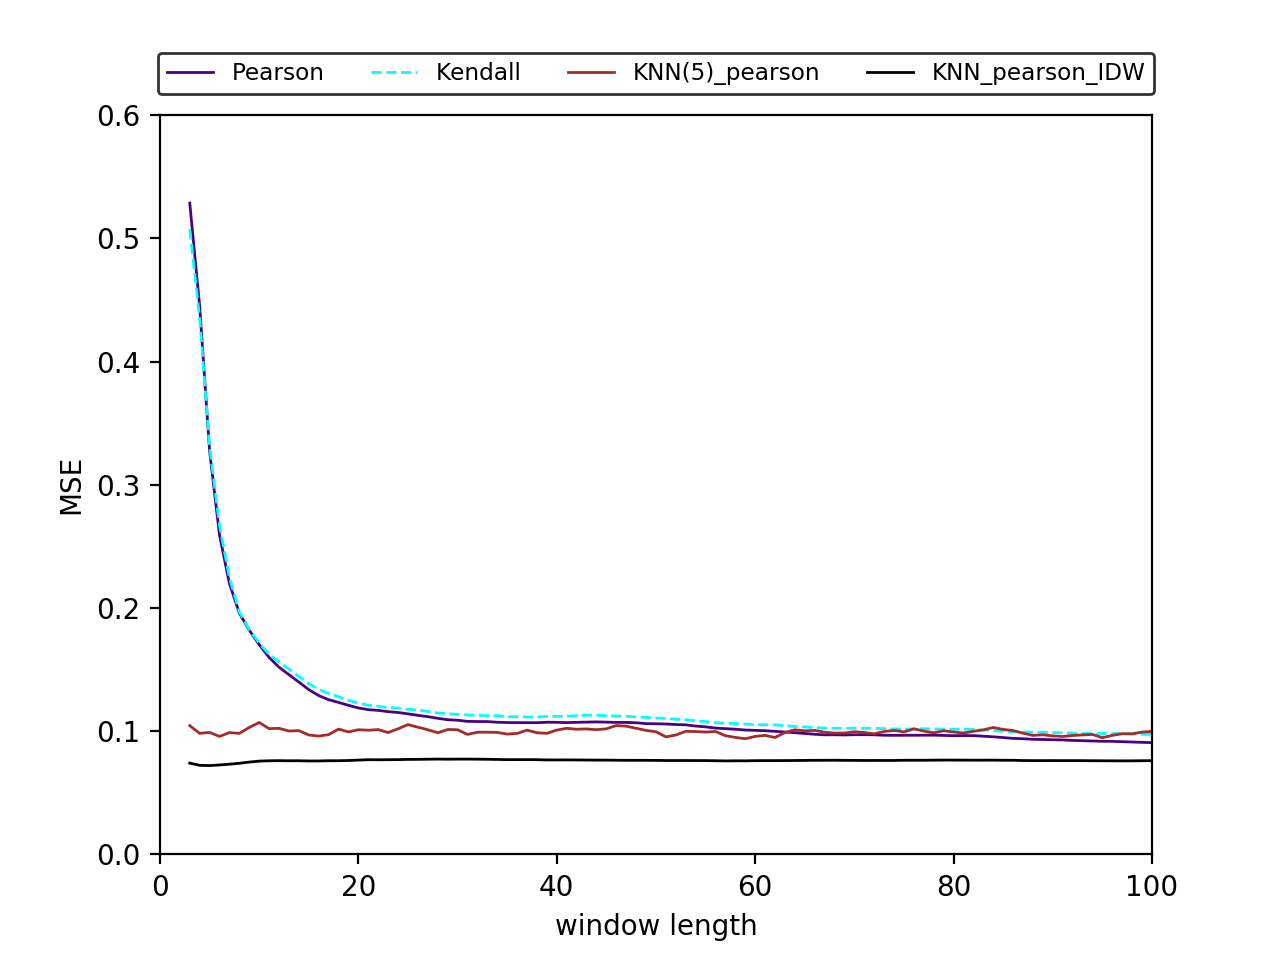
\includegraphics[width=\textwidth]{mse_knn5_idw_pearson_kendall_true} 
		\caption{MSE for KNN with Pearson covariates and true correlation, Pearson and Kendall Moving Window bootstrap estimates.}
		\label{fig:mse_knn5_idw_pearson_kendall_true}
	\end{subfigure}
	\hfill
	\begin{subfigure}[b]{0.49 \textwidth}
		\centering 
		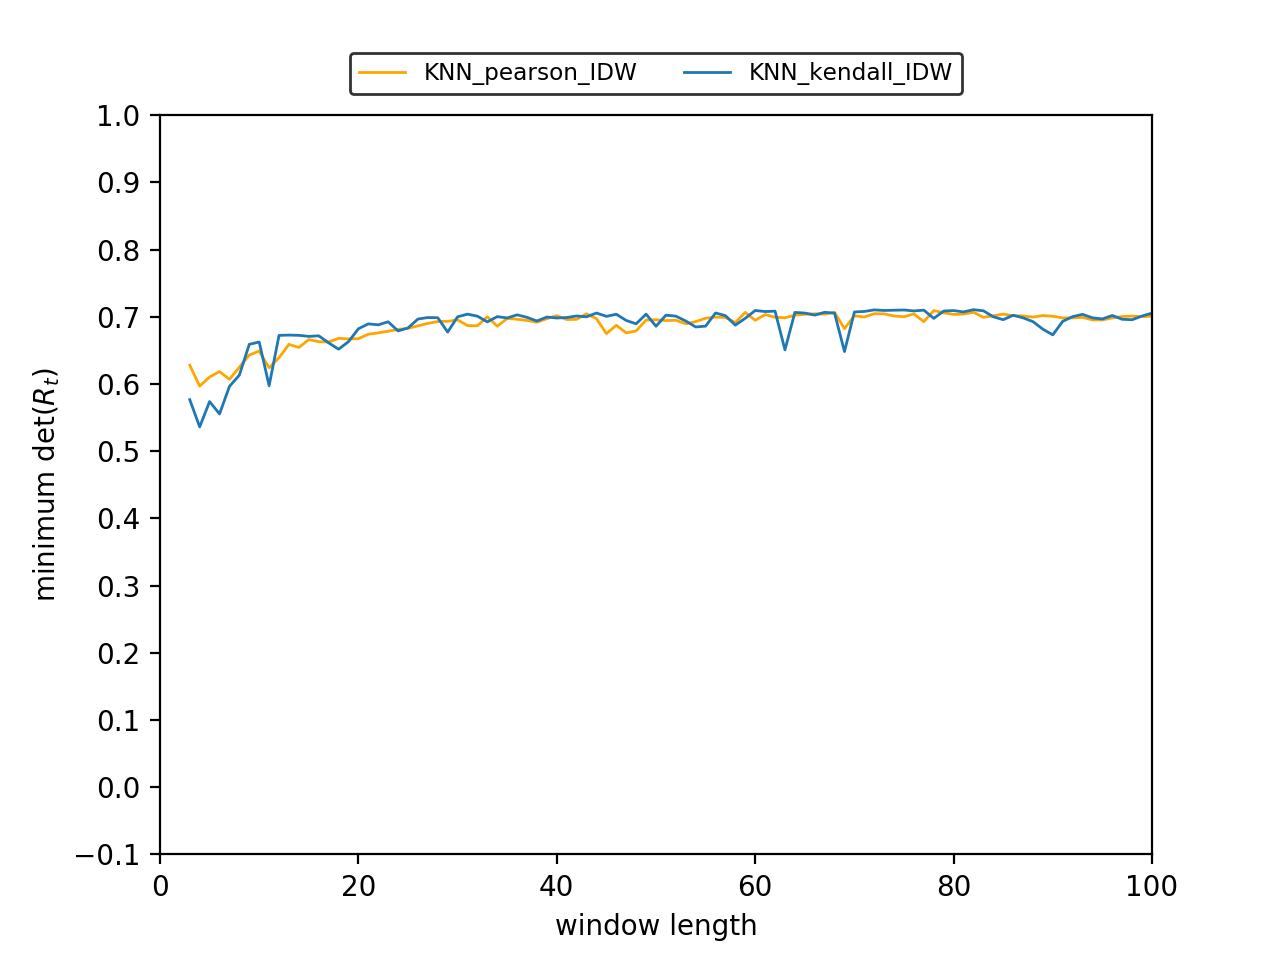
\includegraphics[width=\textwidth]{det_knn_IDW_pearson_kendall_true.png} 
		\caption{Minimum determinants for KNN estimates constructed from inverse distance weighting function, Pearson and Kendall covariates and true correlation.}
		\label{fig:det_knn_IDW_pearson_kendall_true.png}
	\end{subfigure}
	\caption{Comparison MSE and minimum determinants for KNN with true correlation, Pearson and Kendall Moving Window bootstrap estimates.}
	\label{fig:mse_det_knn5_idw_pearson_kendall_true}
\end{figure}


%%%%%%% RANDOM FOREST TRUE COR %%%%%%%%%%%%%%
\subsection{Random Forest}  \label{sec:rf_true_cor}
In order to obtain time-varying correlations, $\rho_t$, with random forests algorithm, the set of covariates is defined by lagged Pearson and Kendall moving window estimates and minimum and maximum asset return values from the last period, denoted by $min_{i,j}(y_{i,j,t-1})$, and $max_{i,j}(y_{i,j,t-1})$, respectively.  \\

\noindent
The accuracy of RF estimates with Pearson and Kendall covariates for time-varying correlation is compared by using mean squared error (MSE) between estimated and actual correlations. MSE from RF with Pearson and Kendall moving window estimates of correlation for covariates are shown in Fig. \ref{fig:mse_rf10_pearson_kendall_true}. Regardless of the choice of window length, MSE from RF with Pearson and Kendall covariates are between 0.0847 and 0.0980, and 0.0830 and 0.0983, respectively. The variance of MSE from RF estimates with Pearson covariates is approximately 8.42e-6 while that of RF estimates with Kendall covariates is approximately 8.92e-6. Analogous to KNN estimates of correlation, RF thus appears to be rather insensitive to the choice of window length, regardless whether the set of covariates is constructed from Pearson or Kendall moving window estimates of correlation. \\

\noindent
Moreover, RF estimates of time-varying correlation where the set of covariates is constructed from Pearson and Kendall moving window estimates and true correlation as output variable satisfy the positive semi-definiteness condition in the time-varying correlation matrix $R_t$ for all time $t$ under all considered choices of window length. Fig. \ref{fig:det_rf10_pearson_kendall_true} presents the obtained minimum determinants of $R_t$ for all choices of window length.   

\begin{figure}[H]
	\centering
	\begin{subfigure}[b]{0.49 \textwidth} 
		\centering
		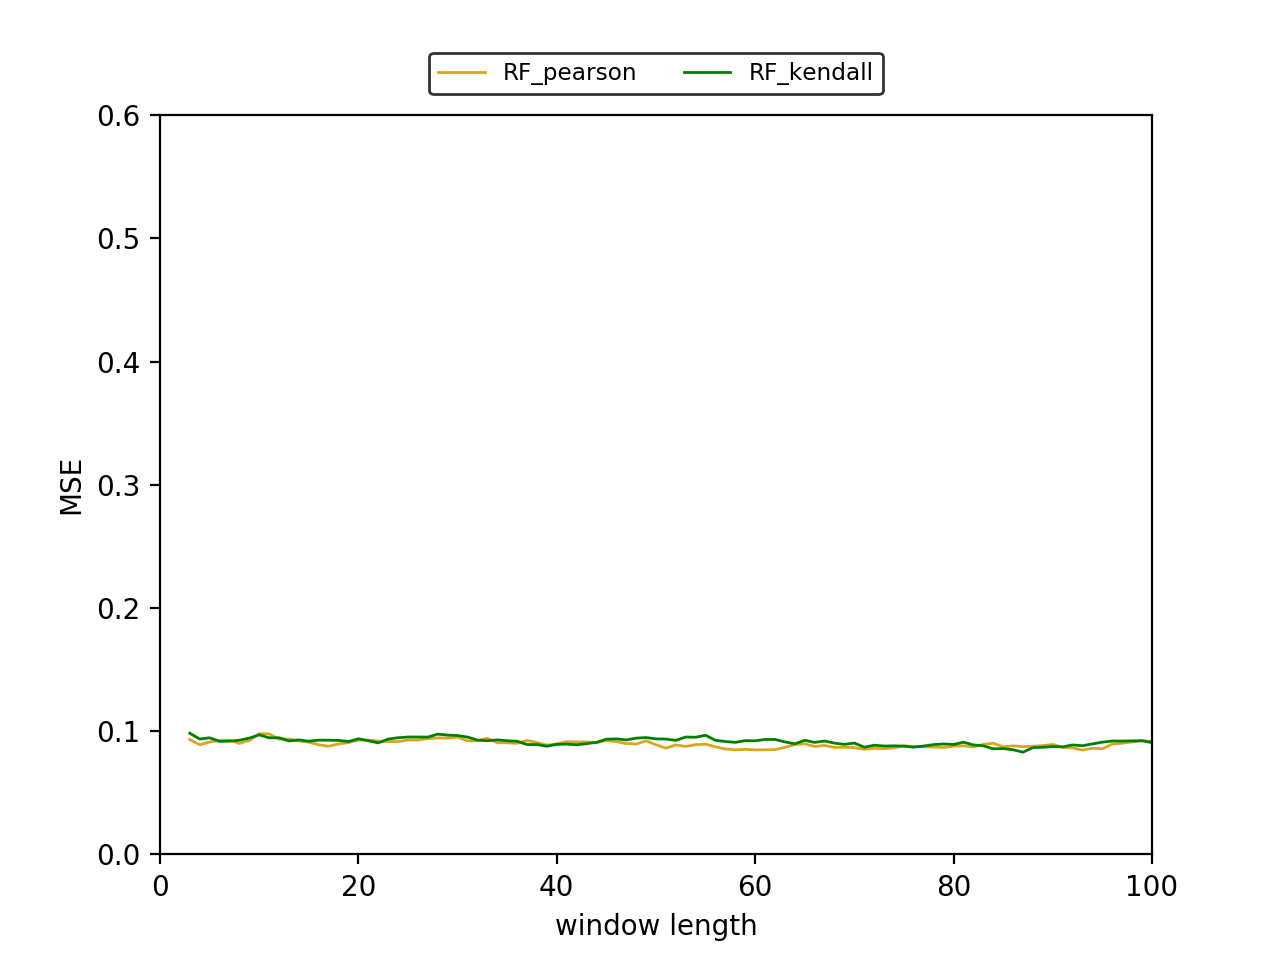
\includegraphics[width=\textwidth]{mse_rf10_pearson_kendall_true}
		\caption{MSE for RF with covariates from Pearson and Kendall and true correlation.}
		\label{fig:mse_rf10_pearson_kendall_true}
	\end{subfigure}
	\hfill
	\begin{subfigure}[b]{0.49 \textwidth} 
		\centering
		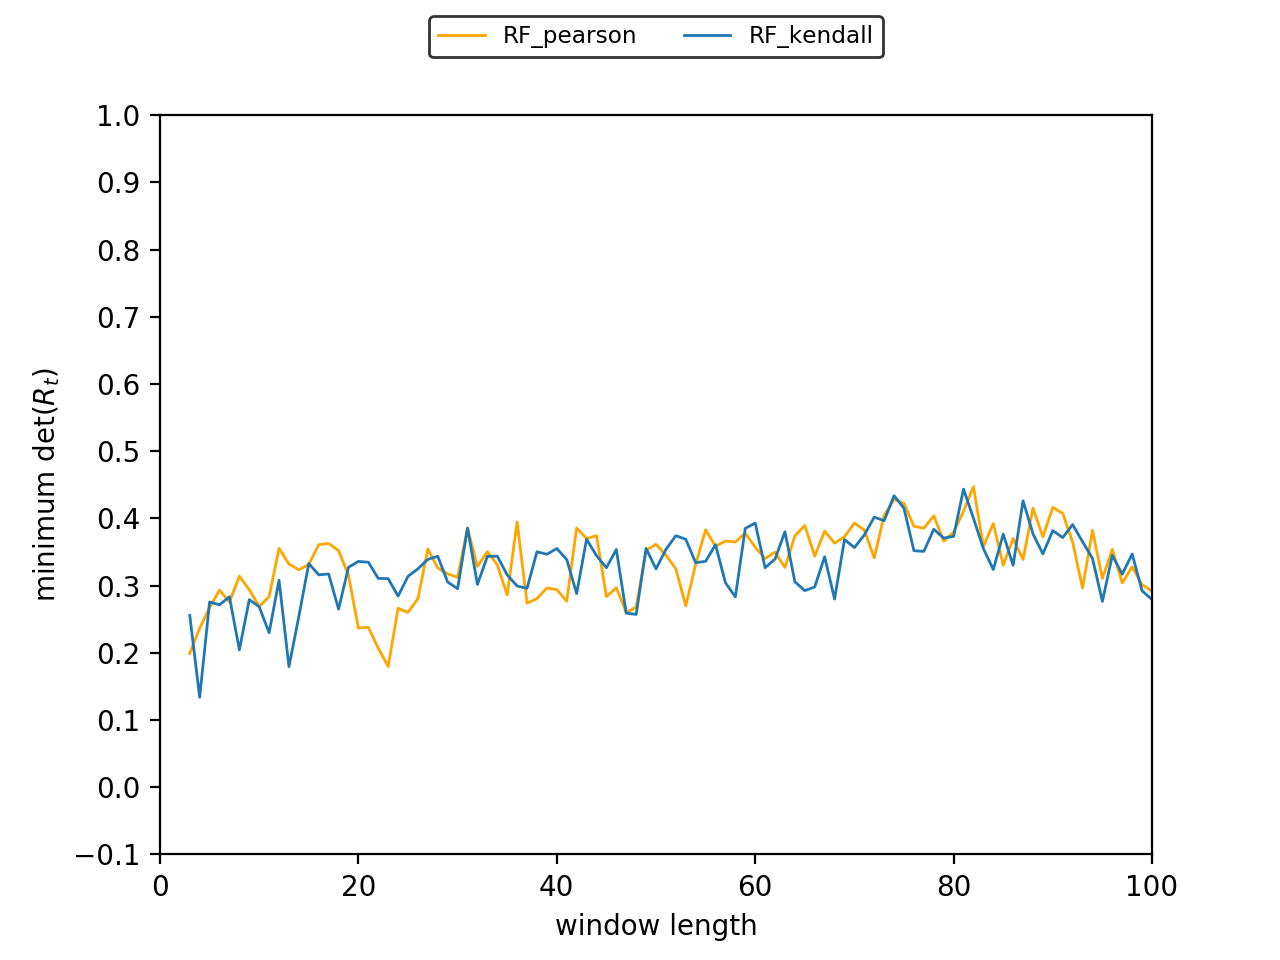
\includegraphics[width=\textwidth]{det_rf10_pearson_kendall_true}
		\caption{Minimum determinants for RF with covariates from Pearson and Kendall and true correlation.}
		\label{fig:det_rf10_pearson_kendall_true}
	\end{subfigure}
	\caption{Comparison MSE and minimum determinants for RF(n\_estimators=10) with covariates from Pearson and Kendall and true correlation.}
	\label{fig:mse_det_rf10_pearson_kendall_true}
\end{figure}

\noindent
From visual inspection of the plots in Fig. \ref{fig:rf_pearson21_bootstrap_true} and Fig. \ref{fig:rf_kendall21_bootstrap_true} it seems that the uncertainty in the time-varying correlation $\rho_t$, which is illustrated by the 99\% confidence interval, seems smaller for RF estimates compared to Pearson and Kendall moving window estimates under the same window length of 21. Analogous to KNN estimates of correlation, RF estimates of correlation with number of trees equal to 10 are much more volatile than Pearson and Kendall moving window estimates. This may be a less desirable result as it is not expected that correlation between assets changes that drastically at each time period. Rather, correlation is expected to vary gradually over time \citep{ref:Basturk2016} \\

\noindent
The MSE decompositions into bias and variance terms from RF estimates of correlation are shown in Fig. \ref{fig:decom_mse_rf10_pearson_true} and Fig. \ref{fig:decom_mse_rf10_kendall_true}. These figures indicate that the RF algorithm is considerably less sensitive to the choice of the window length for smaller window sizes when compared to Pearson and Kendall moving window estimates of correlation depicted in Fig \ref{fig:mse_pearson_kendall_bootstrap}. The uncertainty around the estimated correlations appears to be marginally affected by the choice of the window length for all window sizes. This statement is supported by the fact that the variance as a function of the window length behaves like a (more or less) constant red line in these figures; a result analogous to KNN estimates of correlation.


\begin{figure}[H]  % [h] parameter makes sure figures are located at 'this' location.
	\centering
	\begin{subfigure}[b]{0.49 \textwidth} % sum of widths should be less than text width if all one the same line
		\centering 
		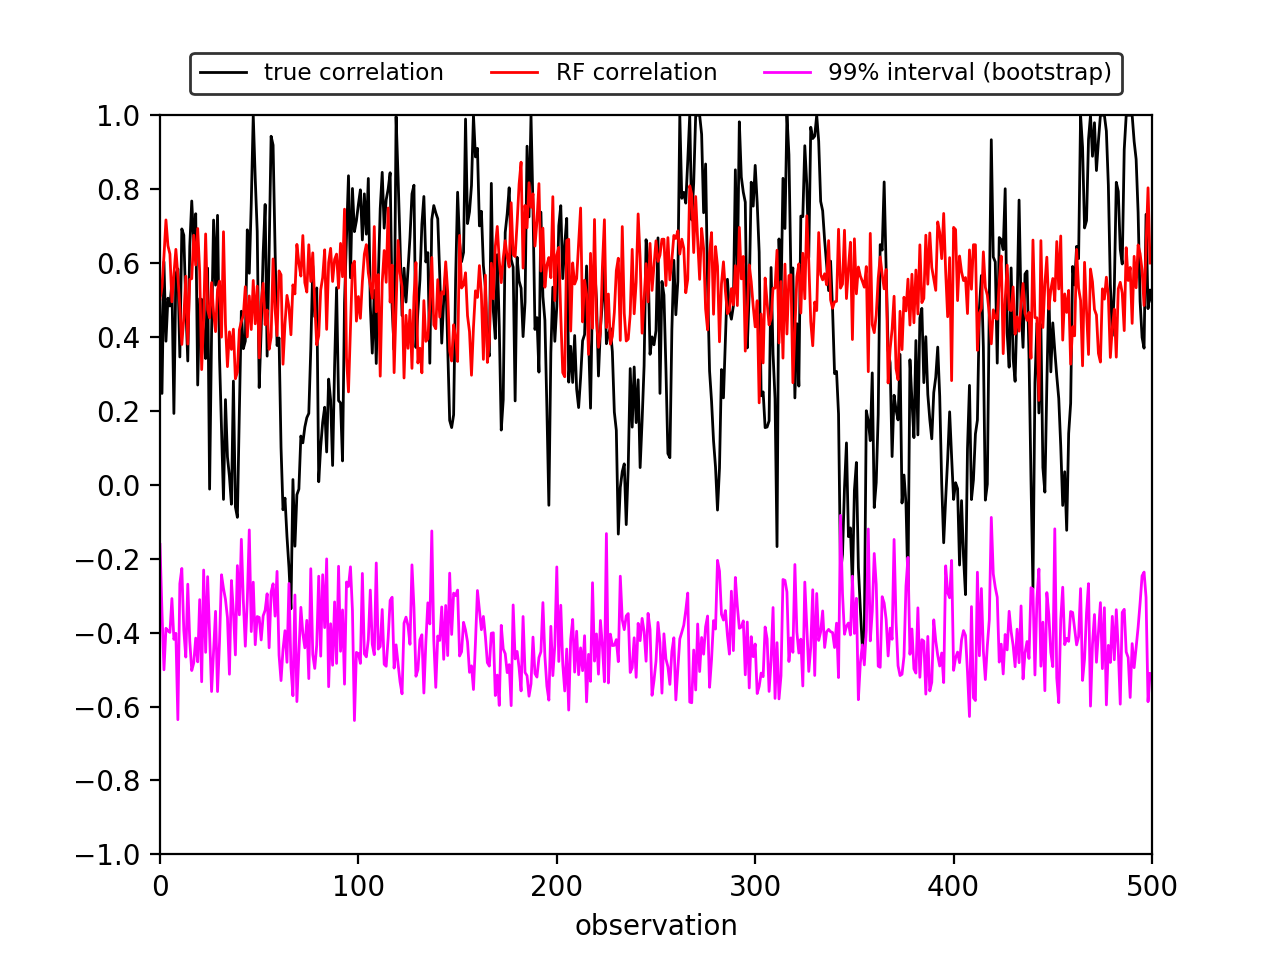
\includegraphics[width=\textwidth]{rf_pearson_21_estimates_bootstrap_true.png} 
		\caption{RF estimates with window size 21, Pearson as covariate and true correlation.} 	
		\label{fig:rf_pearson21_bootstrap_true}
	\end{subfigure} 
	\hfill	
	\begin{subfigure}[b]{0.49 \textwidth} 
		\centering 
		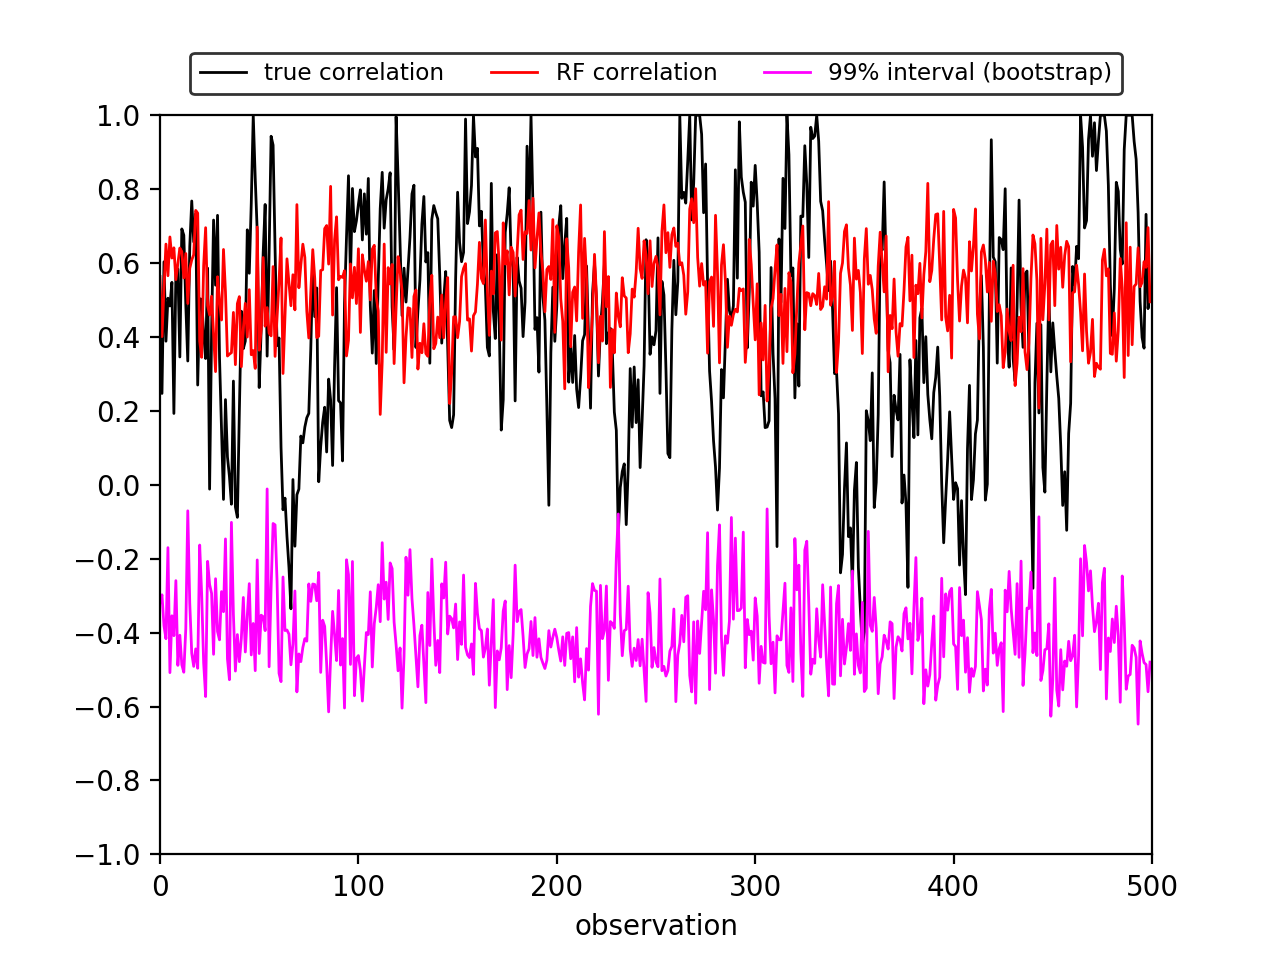
\includegraphics[width=\textwidth]{rf_kendall_21_estimates_bootstrap_true.png} 
		\caption{RF estimates with window size 21, Kendall as covariate and true correlation.} 
		\label{fig:rf_kendall21_bootstrap_true}
	\end{subfigure} 
	\hfill	
	\begin{subfigure}[b]{0.49 \textwidth}
		\centering 		
		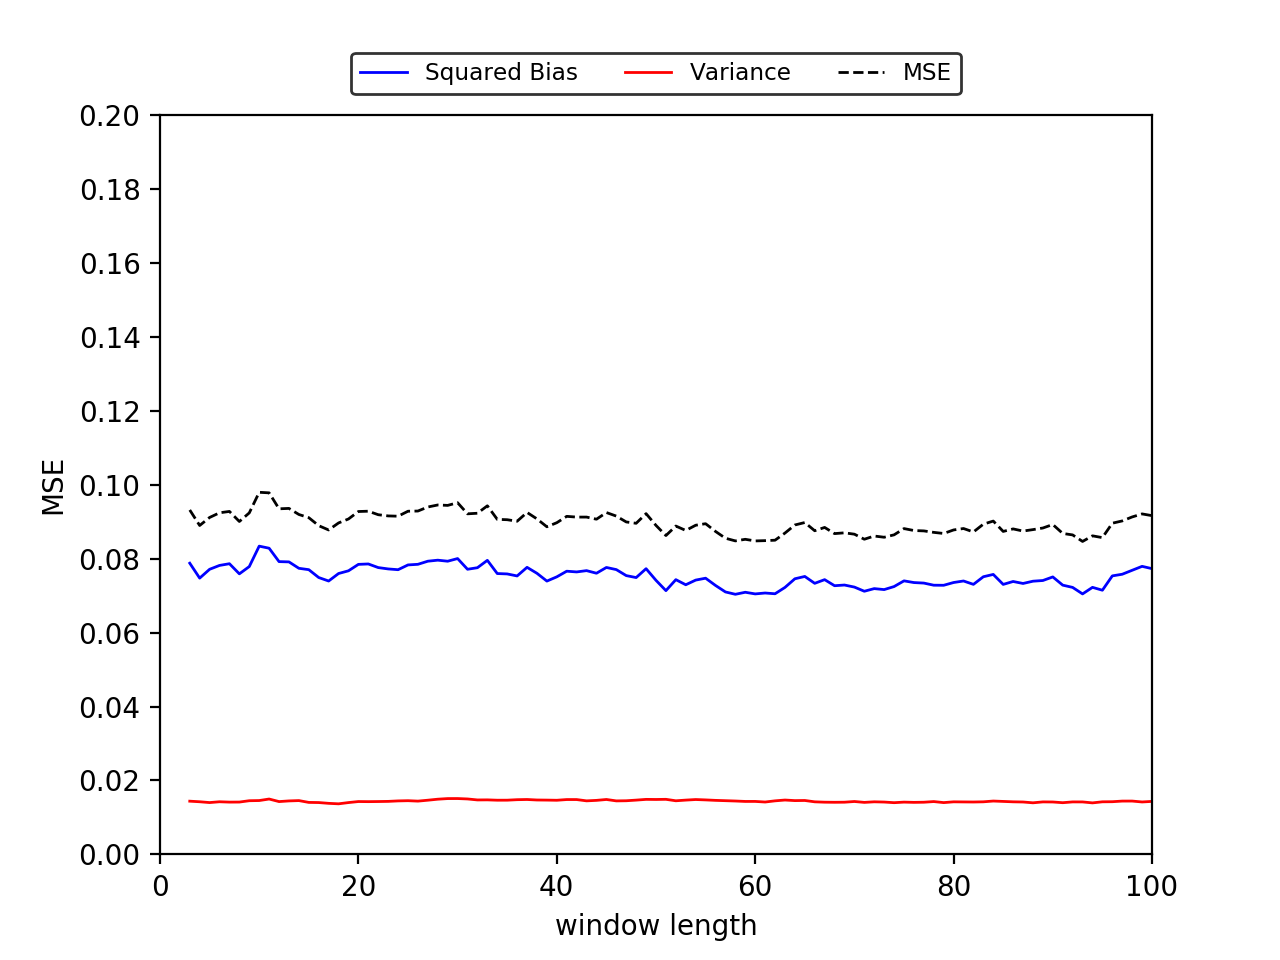
\includegraphics[width=\textwidth]{decom_mse_rf10_pearson_true.png} 
		\caption{Bias-variance decomposition for RF estimates with Pearson as covariate and true correlation.} 
		\label{fig:decom_mse_rf10_pearson_true}
	\end{subfigure}
	\hfill  
	\begin{subfigure}[b]{0.49 \textwidth}
		\centering 
		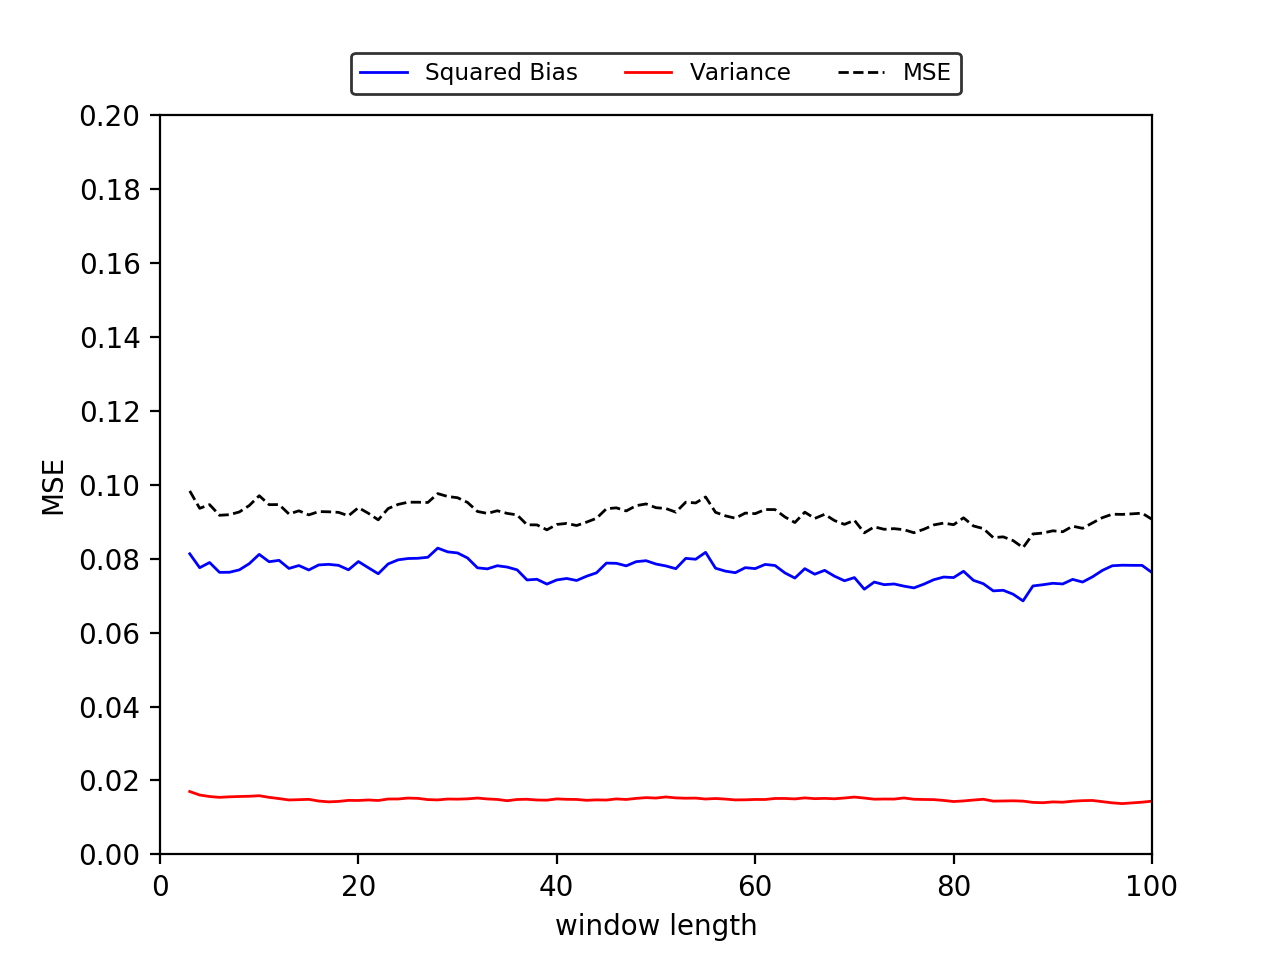
\includegraphics[width=\textwidth]{decom_mse_rf10_kendall_true.png} 
		\caption{Bias-variance decomposition for RF estimates with Kendall as covariate and true correlation.} 
		\label{fig:decom_mse_rf10_kendall_true}
	\end{subfigure}
	\caption{MSE for RF estimates with Pearson and Kendall Moving Window bootstrap estimates as covariates and true correlation.}
	\label{fig:decom_mse_rf10_pearson_kendall_true}
\end{figure}






%%%%%%%%%%%%%%%%%%%%%%%%%%%%%%%%%%%%%
%%%%%%%%%% Proxies for Correlation %%%%%%%%%%%%%%%%
%%%%%%%%%%%%%%%%%%%%%%%%%%%%%%%%%%%%%%
\section{KNN, RF Application with Proxies for Output Variable and Covariates} \label{sec:proxy_correlation}
In this section, a more realistic approach is taken to the application of nearest neighbors and random forests algorithms for time-varying correlation estimation. Both the covariates and output variable are obtained from moving window estimation, as defined in \textbf{Add equation and reference}. This is different from Sec. \ref{sec:true_correlation} where the output variable of the learner models was defined as the true observed correlation (given by the simulated parameters).    

\bigskip
\noindent
\textbf{State what you are precisely going to look at in this section.}
"A fourth issue is the degree of noise in the desired output values (the supervisory target variables). If the desired output values are often incorrect (because of human error or sensor errors), then the learning algorithm should not attempt to find a function that exactly matches the training examples. Attempting to fit the data too carefully leads to overfitting. You can overfit even when there are no measurement errors (stochastic noise) if the function you are trying to learn is too complex for your learning model. In such a situation, the part of the target function that cannot be modeled "corrupts" your training data - this phenomenon has been called deterministic noise. When either type of noise is present, it is better to go with a higher bias, lower variance estimator."

%%%%%% NEAREST neighbor PROXY 	%%%%%%%%
\subsection{Nearest neighbor} \label{sec:knn_proxy_cor}
In this section, results from application of the KNN algorithm will be compared to those obtained by Pearson and Kendall moving window estimation, as depicted in Fig. \ref{fig:decom_mse_pearson_kendall_true}. The uncertainty in the time varying-correlation $\rho_t$, which is illustrated by the 99\% confidence interval, is much smaller compared to MW, even though both the set of covariates and the output variable of the KNN algorithm are based on approximations of correlation instead of actual correlation. \\

\noindent
The accuracy of KNN estimates with Pearson and Kendall moving window estimates for both covariates and output variable is compared by using mean squared error (MSE) between estimated and actual correlations. MSE from KNN with Pearson and Kendall moving window estimates of correlation is shown in Fig. \ref{fig:mse_knn5_pearson_kendall_proxy}. Regardless of the choice of window length, MSE from KNN with Pearson and Kendall covariates are between 0.0855 and 0.2555, and 0.0952 and 0.2223, respectively. The variance of MSE from KNN estimates with Pearson covariates is approximately 5.70e-4 while that of KNN estimates with Kendall covariates is approximately 2.96e-4. Recall that in Fig. \ref{fig:mse_knn5_pearson_kendall_true} KNN appeared to be insensitive to the choice of window length when true correlation is defined as the output variable. Interestingly, Fig. \ref{fig:mse_knn5_pearson_kendall_proxy} shows that MSE from KNN estimation with Pearson or Kendall approximations for the output variable varies substantially for smaller window sizes. Although, less variation is observed when compared with MSE from Pearson and Kendall moving window estimates depicted in Fig. \ref{fig:mse_pearson_kendall_bootstrap}. A possible explanation for this behaviour will be given towards the end of this section when comparing MSE between KNN estimates and Pearson and Kendall moving window estimates in more detail. \\

\noindent
Moreover, KNN estimates of time-varying correlation where the set of covariates is constructed from Pearson and Kendall moving window estimates and proxy correlation, satisfy the positive semi-definiteness condition in the time-varying correlation matrix $R_t$ for all time $t$ under all choices of window length. Fig. \ref{fig:det_knn5_pearson_kendall_proxy} presents the obtained minimum determinants of $R_t$ for all choices of window length.  
     
\begin{figure}[H]
	\centering
	\begin{subfigure}[b]{0.49 \textwidth} 
		\centering
		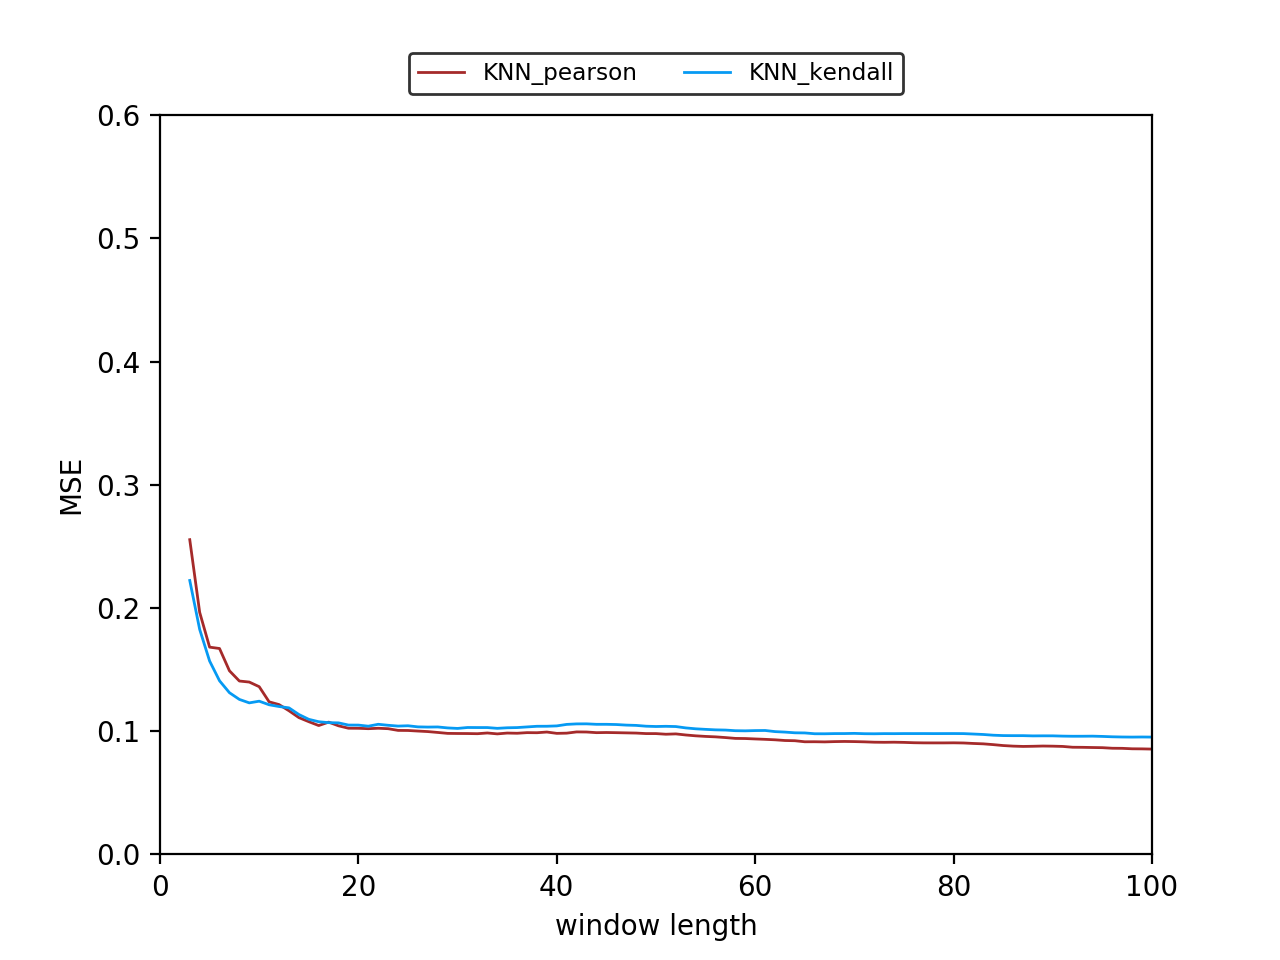
\includegraphics[width=\textwidth]{mse_knn5_pearson_kendall_proxy.png}
		\caption{MSE for KNN with covariates from Pearson and Kendall and proxy correlation.}
		\label{fig:mse_knn5_pearson_kendall_proxy}
	\end{subfigure}
	\hfill
	\begin{subfigure}[b]{0.49 \textwidth} 
		\centering
		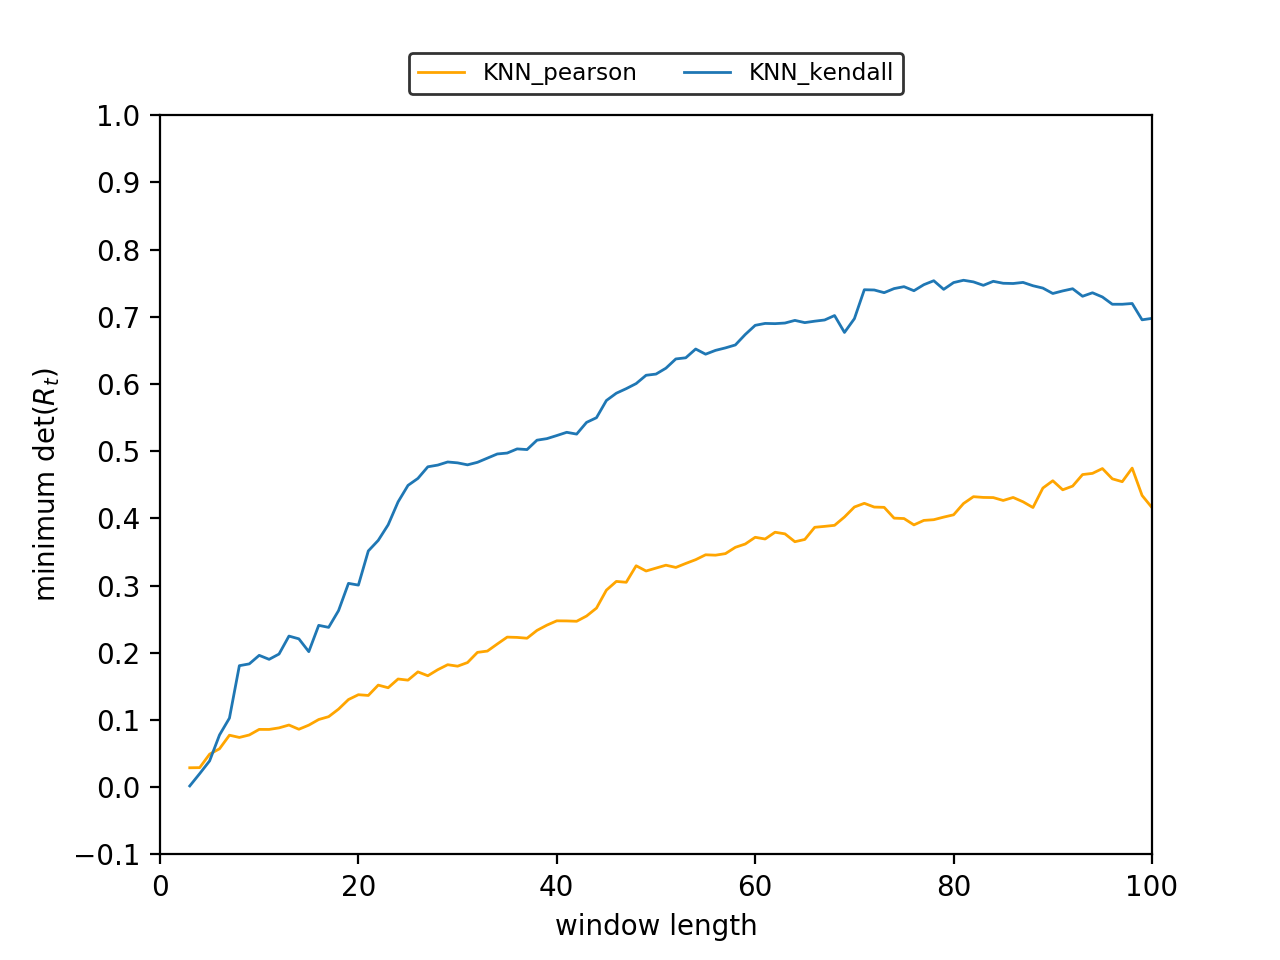
\includegraphics[width=\textwidth]{det_knn5_pearson_kendall_proxy}
		\caption{Minimum determinants for KNN with covariates from Pearson and Kendall and proxy correlation.}
		\label{fig:det_knn5_pearson_kendall_proxy}
	\end{subfigure}	
	\caption{Comparison MSE and minimum determinants for KNN(n\_neighbors=5) with covariates from Pearson and Kendall and proxy correlation.}
	\label{fig:mse_det_knn5_pearson_kendall_proxy}
\end{figure}

\noindent
From visual inspection of the plots in Fig. \ref{fig:knn_pearson21_bootstrap_proxy} and Fig. \ref{fig:knn_kendall21_bootstrap_proxy} it is clear that the uncertainty in the time-varying correlation $\rho_t$, 
which is illustrated by the $99\%$ confidence interval, is smaller for KNN estimates compared to Pearson moving window estimates and Kendall moving window estimates, even though both the set of covariates and the output variable of the KNN algorithm are based on approximations of correlation instead of actual correlation. These figures also show smaller uncertainty in the time-varying correlation $\rho_t$ when compared with KNN estimates with true correlation as the output variable, which are depicted in Fig. \ref{fig:decom_mse_knn5_pearson_kendall_proxy}. KNN estimates of correlation with true correlation as output variable in Fig. \ref{fig:knn_pearson21_bootstrap_proxy} and Fig. \ref{fig:knn_kendall21_bootstrap_proxy} are much more volatilte. KNN estimates with approximated correlation as output variable in Fig. \ref{fig:knn_pearson21_bootstrap_proxy} and Fig. \ref{fig:knn_kendall21_bootstrap_proxy}, however, follow the increases and decreases of the actual correlation smoother, with tighter confidence intervals. This is a more desirable result as it is not expected that correlation between assets changes that drastically at each time period. \\


\noindent
The MSE decompositions into bias and variance terms from KNN estimates of correlation are shown in Fig. \ref{fig:decom_mse_knn_pearson_proxy} and Fig. \ref{fig:decom_mse_knn_kendall_proxy}. These figures indicate that the KNN algorithm with approximated output is more sensitive to the choice of the window length for smaller window sizes compared to KNN algorithm with true correlation depicted in Fig. \ref{fig:decom_mse_knn5_pearson_kendall_true}. This observation can be explained by error propagation: the effect of covariates' uncertainties (or errors) on the error of the function based on them. In the case when KNN algorithm uses proxies for output variables, the error associated with approximation of true correlation using moving window estimates is propagated to the output of the KNN algorithm. Fig. \ref{fig:decom_mse_knn_pearson_proxy} and Fig. \ref{fig:decom_mse_knn_kendall_proxy} show, however, that the KNN algorithm with approximated output is considerably less sensitive to the choice of the window length for smaller window sizes when compared to Pearson and Kendall moving window estimates of correlation depicted in Fig. \ref{fig:decom_mse_pearson} and Fig \ref{fig:decom_mse_kendall}, respectively. The KNN algorithm thus seems to mitigate the error propagation to some extend for smaller window sizes. This may be due to the fact that KNN, even with a small number of neighbors such as the default value of 5, estimates time-varying correlation using neighbors that contain additional informational value compared to the informational value in moving window estimates with small window sizes.      


\begin{figure}[H]  % [h] parameter makes sure figures are located at 'this' location.
	\centering
	\begin{subfigure}[b]{0.49 \textwidth} % sum of widths should be less than text width if all one the same line
		\centering 
		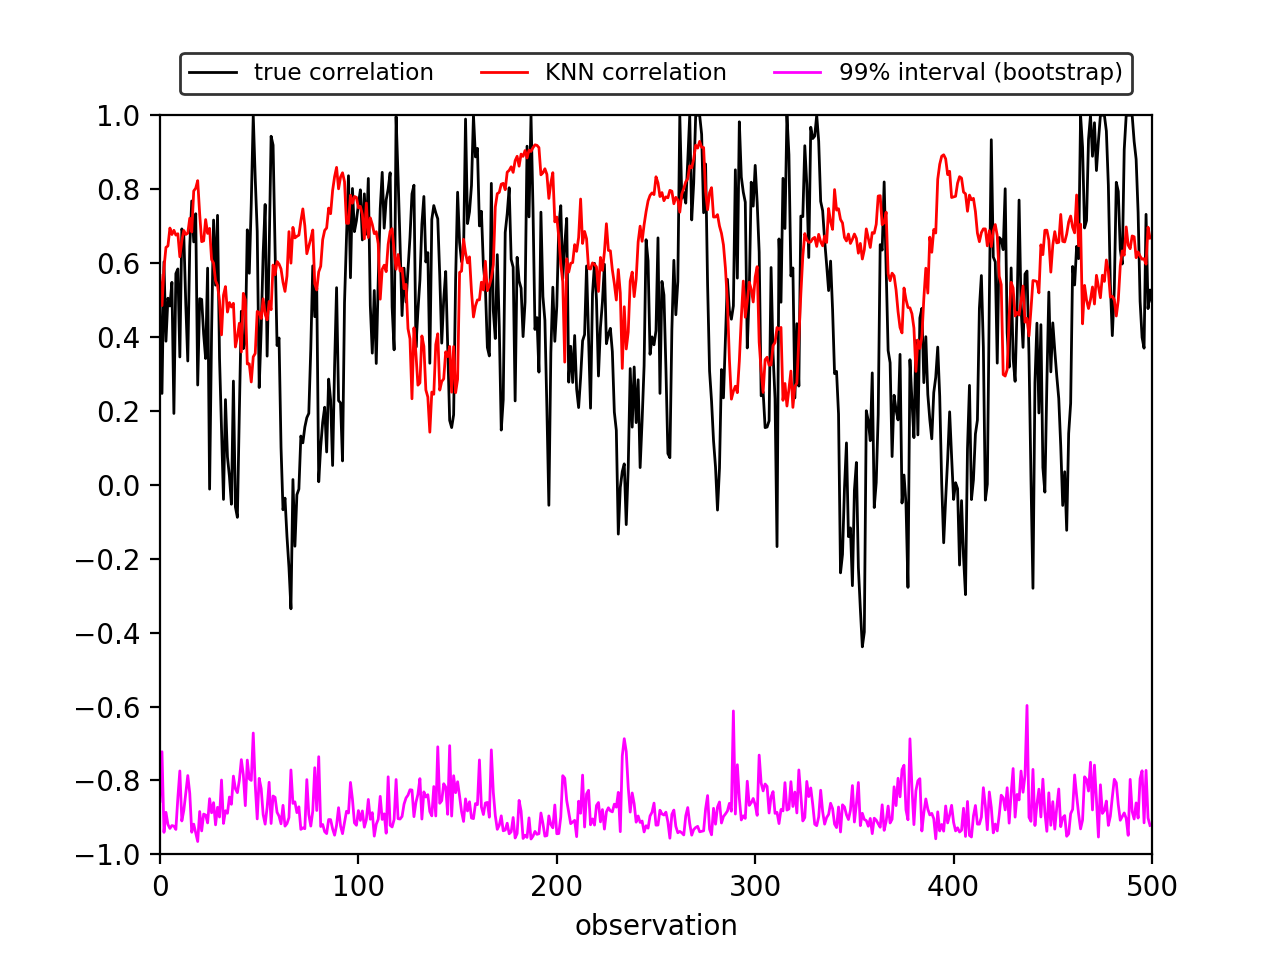
\includegraphics[width=\textwidth]{knn_pearson_21_estimates_bootstrap_proxy.png} 
		\caption{KNN estimates with window size 21, Pearson as covariate and proxy correlation.} 	
		\label{fig:knn_pearson21_bootstrap_proxy}
	\end{subfigure} 
	\hfill	
	\begin{subfigure}[b]{0.49 \textwidth} 
		\centering 
		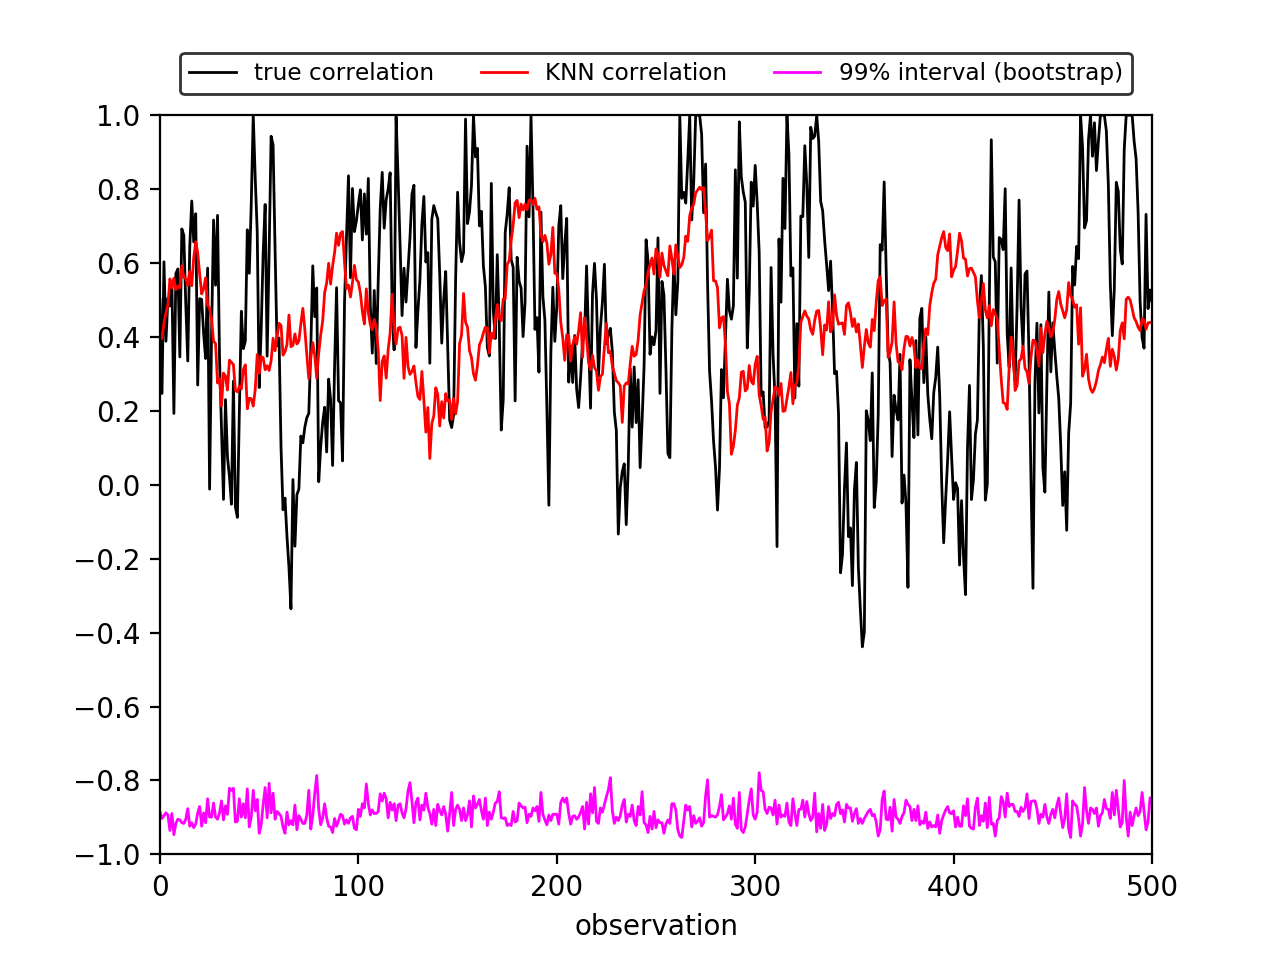
\includegraphics[width=\textwidth]{knn_kendall_21_estimates_bootstrap_proxy.png} 
		\caption{KNN estimates with window size 21, Kendall as covariate and proxy correlation.} 
		\label{fig:knn_kendall21_bootstrap_proxy}
	\end{subfigure} 
	\hfill	
	\begin{subfigure}[b]{0.49 \textwidth}
		\centering 
		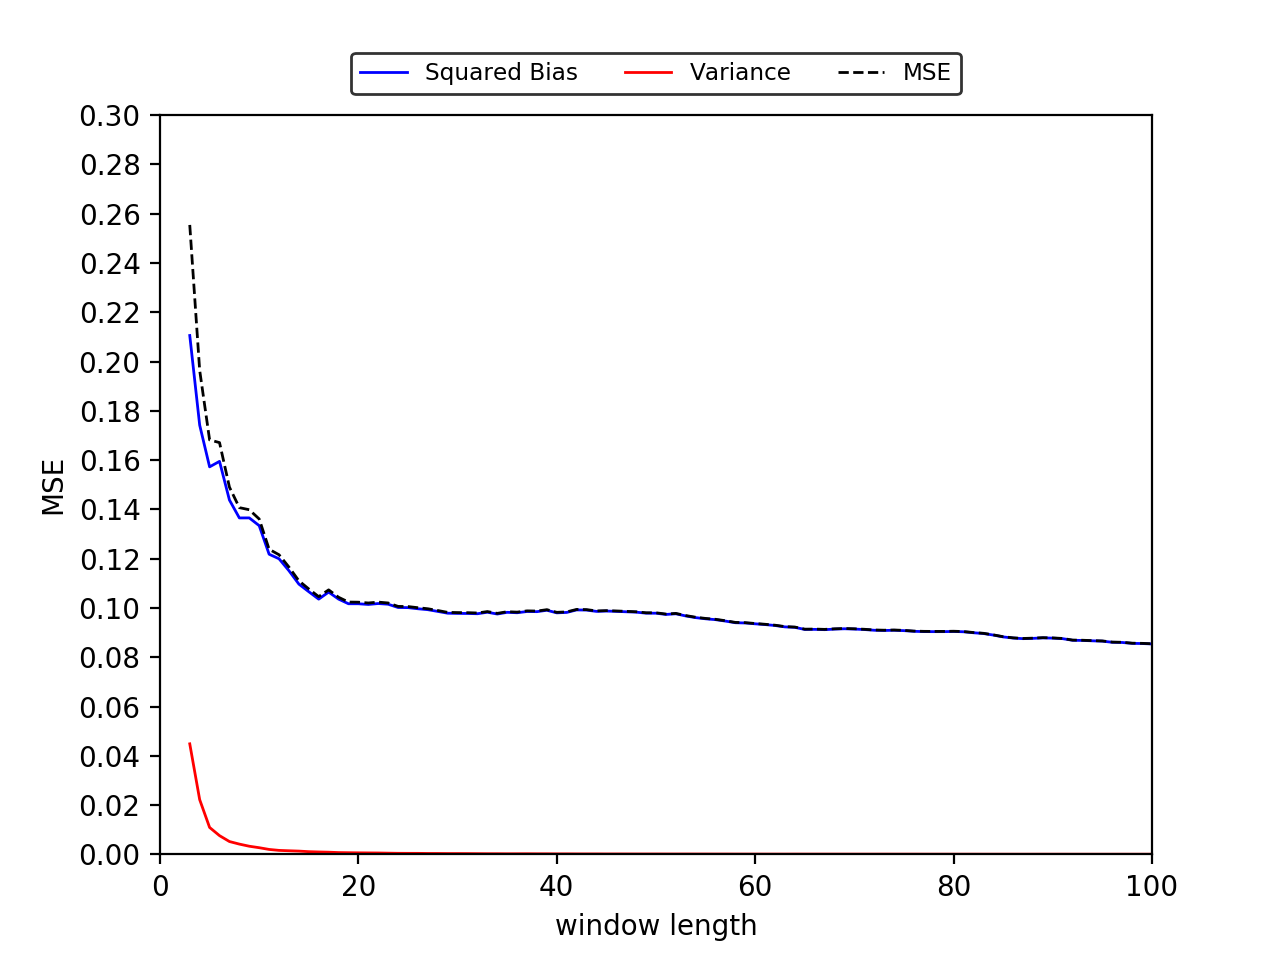
\includegraphics[width=\textwidth]{decom_mse_knn_pearson_proxy.png} 
		\caption{Bias-variance decomposition for KNN estimates with Pearson as covariate and proxy correlation.} 	
		\label{fig:decom_mse_knn_pearson_proxy}
	\end{subfigure}
	\hfill  
	\begin{subfigure}[b]{0.49 \textwidth}
		\centering 
		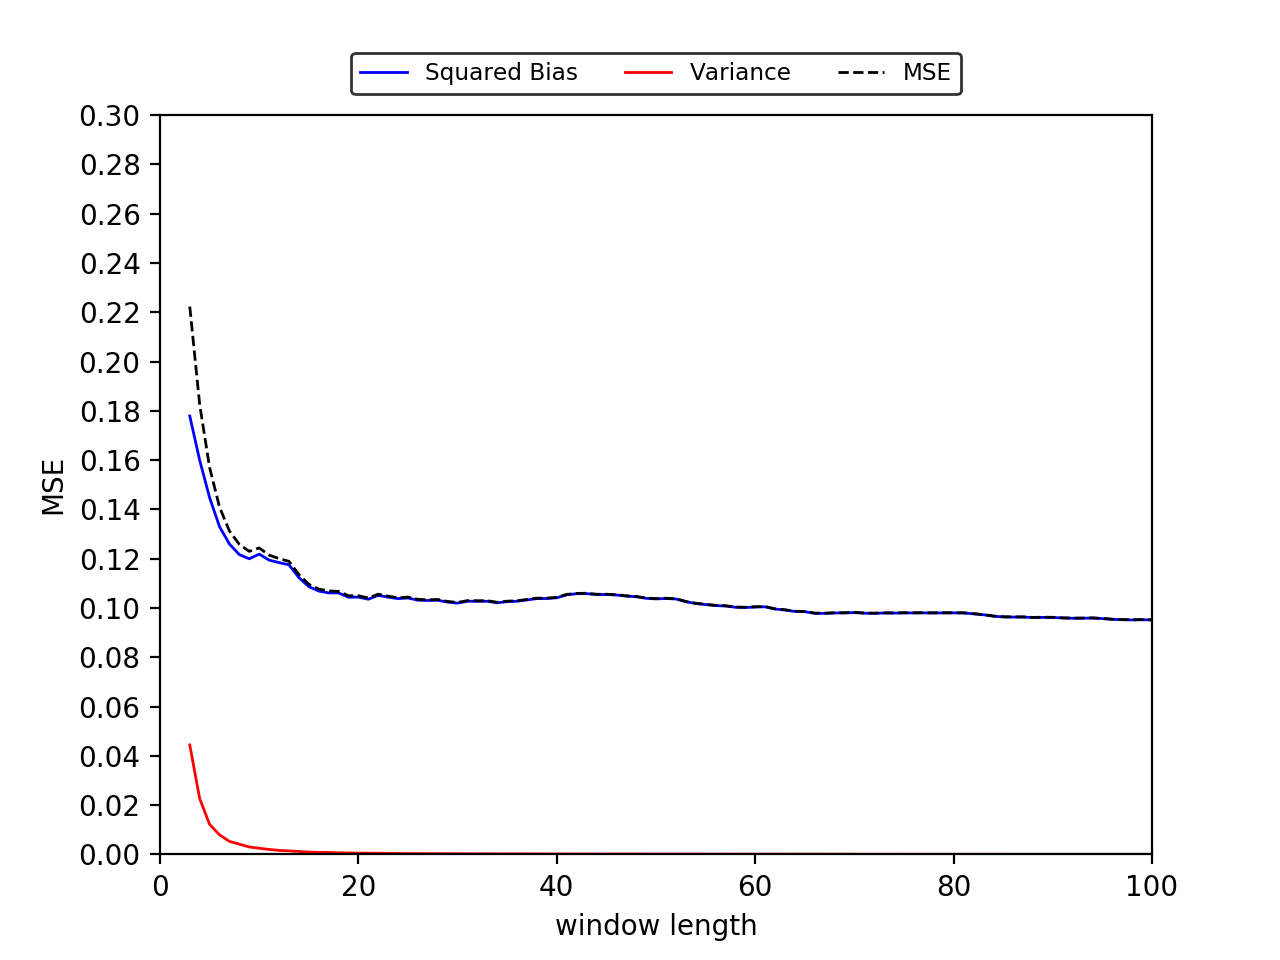
\includegraphics[width=\textwidth]{decom_mse_knn_kendall_proxy.png} 
		\caption{Bias-variance decomposition for KNN estimates with Kendall as covariate and proxy correlation.} 
		\label{fig:decom_mse_knn_kendall_proxy}
	\end{subfigure}
	\caption{MSE for KNN estimates with Pearson and Kendall Moving Window bootstrap estimates as covariates and proxy correlation.}
	\label{fig:decom_mse_knn5_pearson_kendall_proxy}
\end{figure}

\noindent
Tabel \ref{tab:mse_decomp_knn_pearson_kendall_proxy} presents MSE decomposition as a function of number of neighbors $k$ for KNN estimates with approximations for both covariates and output variable. Similar results are observed for $k \in \{5, 10, 25, 50, 100\}$ when compared with KNN estimates with approximated covariates and true correlation in Tabel \ref{tab:mse_decomp_knn_pearson_kendall_true}; both squared bias and variance decrease with an increase in $k$, and conversely, regardless whether Pearson or Kendall estimates are used for defining the set of covariates. Given Eq. \eqref{eq:mse_decomposition_knn} and our discussion from Section \ref{sec:mse_decompose} one might have expected an increase in squared bias with an increase in $k$. A possible explanation for this behaviour may be that up to some $k$, an increase in $k$ implies additional neighbors containing informational value are used for the estimation of time-varying correlations. Logically, the inclusion of additional neighbors containing informational value results into more accurate estimates of correlation, i.e. a decrease in squared bias. As of some $k$, however, additional neighbors only add noise to the estimation process which results into increased squared bias. For KNN estimates with Kendall covariate and proxy correlation this is for $k = 900$ whereas squared bias still decreases for $k = 1000$ in the case of KNN estimates with Pearson covariate and proxy correlation. Given our discussion from Section \ref{sec:mse_decompose} and results from KNN estimates with approximated covariates and true correlation in Tabel \ref{tab:mse_decomp_knn_pearson_kendall_true}, one might have expected a continuing decrease in variance with an increase in $k$. Interestingly, Tabel \ref{tab:mse_decomp_knn_pearson_kendall_proxy} shows an increase in variance from $k = 800$ and $k = 900$ onwards for KNN estimates with Pearson and Kendall covariates, respectively.          


%% TABLE
\begin{table}[H]
\centering
\captionsetup[subtable]{position=below}
%\captionsetup[table]{position=below}
\begin{subtable}{0.49\linewidth}
\centering
\begin{tabular}{r  c  c  c} 
\toprule
\multicolumn{1}{ r }{\textbf{k}} &
\multicolumn{1}{ c }{\textbf{Squared Bias}} &
\multicolumn{1}{ c }{\textbf{Variance}} &
\multicolumn{1}{ c }{\textbf{MSE}} \\
\midrule 

5                                     & 0.1334                         & 0.0027                & 0.1361     \\
10                                   & 0.1319                         & 0.0015                & 0.1334     \\
25                                   & 0.1289 	                    & 6.64e-4                & 0.1295     \\
50                                   & 0.1268                         & 3.57e-4                & 0.1271     \\
100                                 & 0.1238                         & 1.95e-4               & 0.1240      \\
200                                 & 0.1169                         & 1.14e-4               & 0.1170      \\
400                                 & 0.1047                         & 7.80e-5               & 0.1048      \\
600                                 & 0.0946                         & 7.20e-5               & 0.0947     \\
800                                 & 0.0870                         & 7.50e-5               & 0.0870      \\
900				     & 0.0841			   & 8.00e-5              & 0.0842      \\
1000                               & 0.0827                         & 8.80e-5              & 0.0828     \\ [1ex]
\bottomrule
\end{tabular}
\caption{MSE for KNN estimates with window size 10, Pearson as covariate and correlation.}
\label{tab:mse_decomp_knn_pearson_proxy}
\end{subtable}
\hfill
\begin{subtable}{0.49\linewidth}
\centering
\begin{tabular}{r  c  c  c} 
\toprule
\multicolumn{1}{ r }{\textbf{k}} &
\multicolumn{1}{ c }{\textbf{Squared Bias}} &
\multicolumn{1}{ c }{\textbf{Variance}} &
\multicolumn{1}{ c }{\textbf{MSE}} \\
\midrule 

5                                     & 0.1219                         &  0.0025              & 0.1244   \\
10                                   & 0.1200                         & 0.0014               & 0.1214   \\
25                                   & 0.1183	                   & 5.98e-4              & 0.1189    \\
50                                   & 0.1168                        & 3.17e-4	       & 0.1171    \\
100                                 & 0.1148                         & 1.75e-4              & 0.1150    \\
200                                 & 0.1110                        & 1.02e-4              & 0.1110    \\
400                                 & 0.1042                        & 6.80e-5             & 0.1043   \\
600                                 & 0.0998                         & 6.00e-5             & 0.0998     \\
800                                 & 0.0969                         & 5.90e-5             & 0.0970    \\
900				     & 0.0969			   & 6.00e-5             & 0.0970     \\
1000                               & 0.0988                       & 6.30e-5             & 0.0988     \\  [1ex]
\bottomrule
\end{tabular}
\caption{MSE for KNN estimates with window size 10, Kendall as covariate and correlation.}
\label{tab:mse_decomp_knn_kendall_proxy}
\end{subtable}
\caption{Mean Squared Error (MSE) decomposition as a function of the number of neighbors (k) for KNN with approximations for both covariates and output variable.}
\label{tab:mse_decomp_knn_pearson_kendall_proxy}
\end{table}

\noindent
As in Section \ref{sec:knn_true_cor}, two more parameterisations of the KNN learner model are analysed where the set of neighbors used for point estimation of time-varying correlation is defined as the entire training set. The KNN algorithm uses an uniformly weighted average of correlations and an inverse distance weighted average of correlations, as defined in Eq. \ref{eq:IDWfunction} \citep{ref:Shepard1968} in the first and second parameterisation, respectively. The MSE decompositions of both parameterisations with proxies for covariates and the output variable is depicted in Fig. \ref{fig:decom_mse_knn_len_train_IDW_pearson_kendall_proxy}. The variance term becomes negligible small in case the set of neighbors used for point estimation of time-varying correlation is defined as the entire training set, regardless of the weighting function. The red line of the variance is barely observable in the bottom of Fig. \ref{fig:decom_mse_knn_len_train_pearson_proxy}-\ref{fig:decom_mse_knn_IDW_kendall_proxy}. This is in line with results presented in Tabel \ref{tab:mse_decomp_knn_pearson_kendall_proxy} where the value of the variance term is negligible small for larger $k$, regardless whether the set of covariates is constructed from Pearson or Kendall moving window estimates of correlation.
     


\begin{figure}[H]  % [h] parameter makes sure figures are located at 'this' location.
	\centering
	\begin{subfigure}[b]{0.49 \textwidth}
		\centering 
		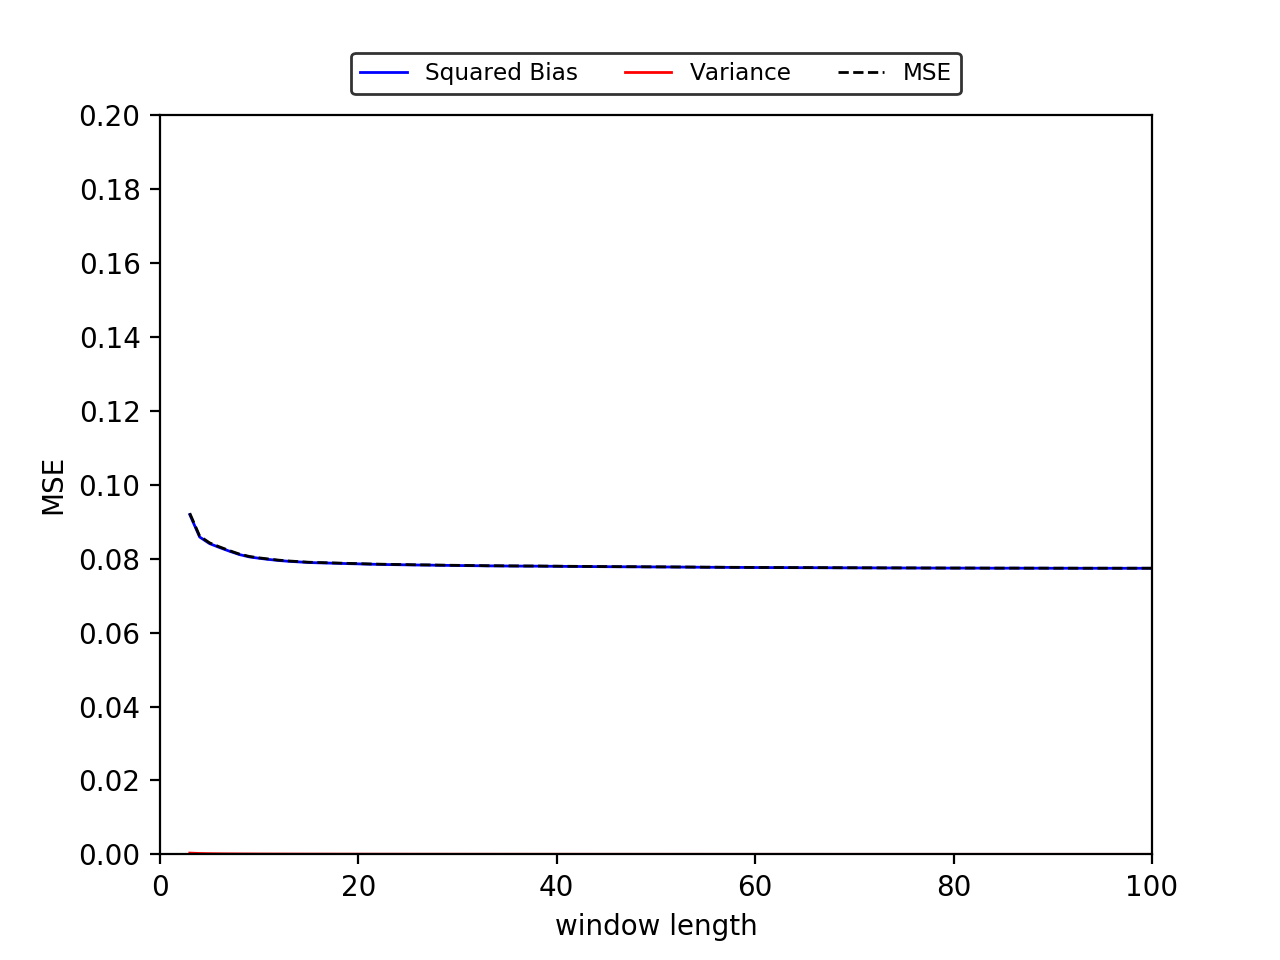
\includegraphics[width=\textwidth]{decom_mse_knn_len_train_pearson_proxy.png} 
		\caption{Bias-variance decomposition for KNN estimates constructed from uniformly weighted averages and Pearson covariates.} 	
		\label{fig:decom_mse_knn_len_train_pearson_proxy}
	\end{subfigure}
	\hfill  
	\begin{subfigure}[b]{0.49 \textwidth}
		\centering 
		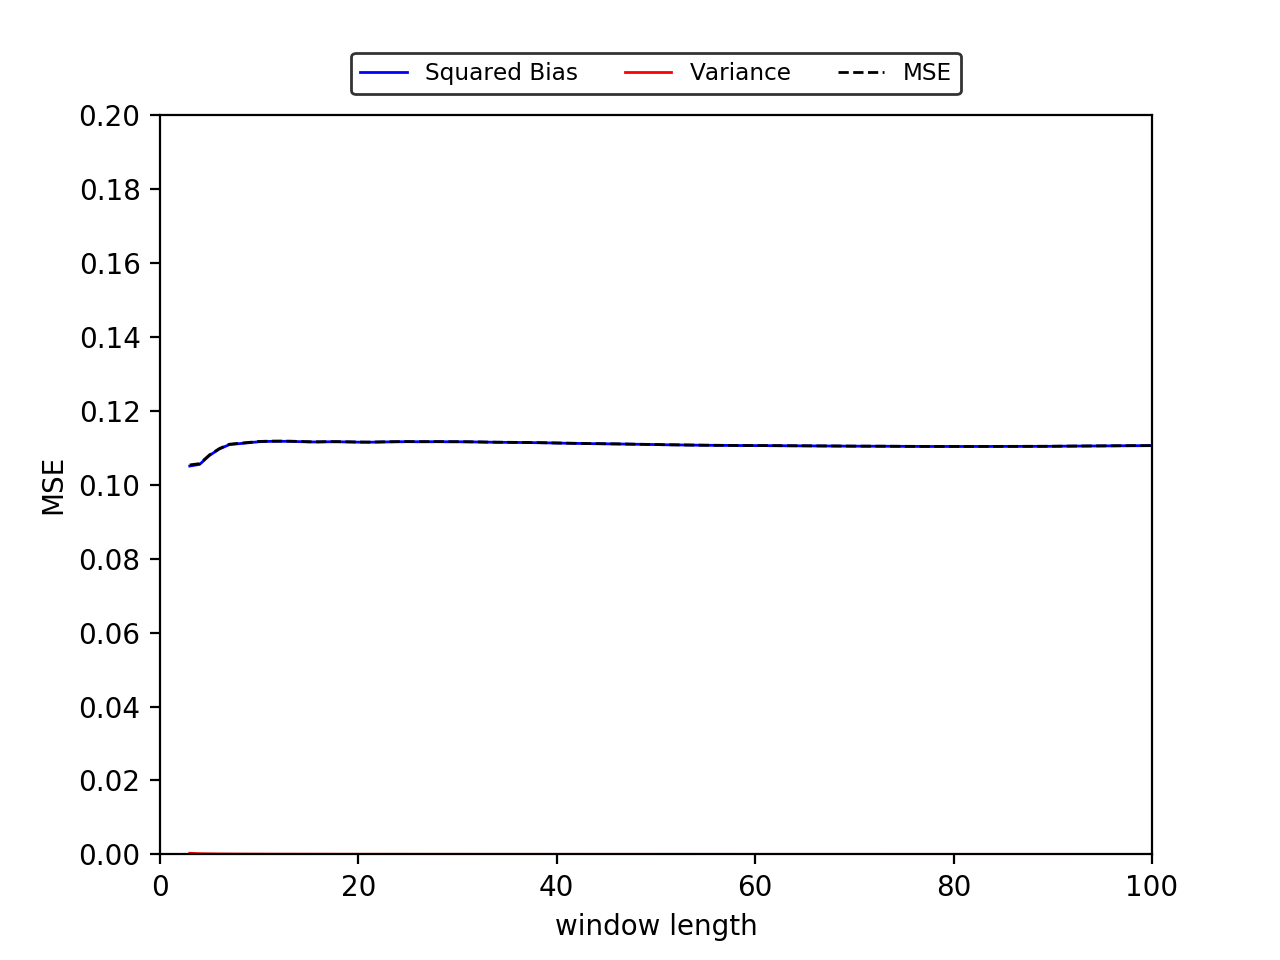
\includegraphics[width=\textwidth]{decom_mse_knn_len_train_kendall_proxy.png} 
		\caption{Bias-variance decomposition for KNN estimates constructed from uniformly weighted averages  and Kendall covariates.} 
		\label{fig:decom_mse_knn_len_train_kendall_proxy}
	\end{subfigure}
	\hfill  
	\begin{subfigure}[b]{0.49 \textwidth}
		\centering 
		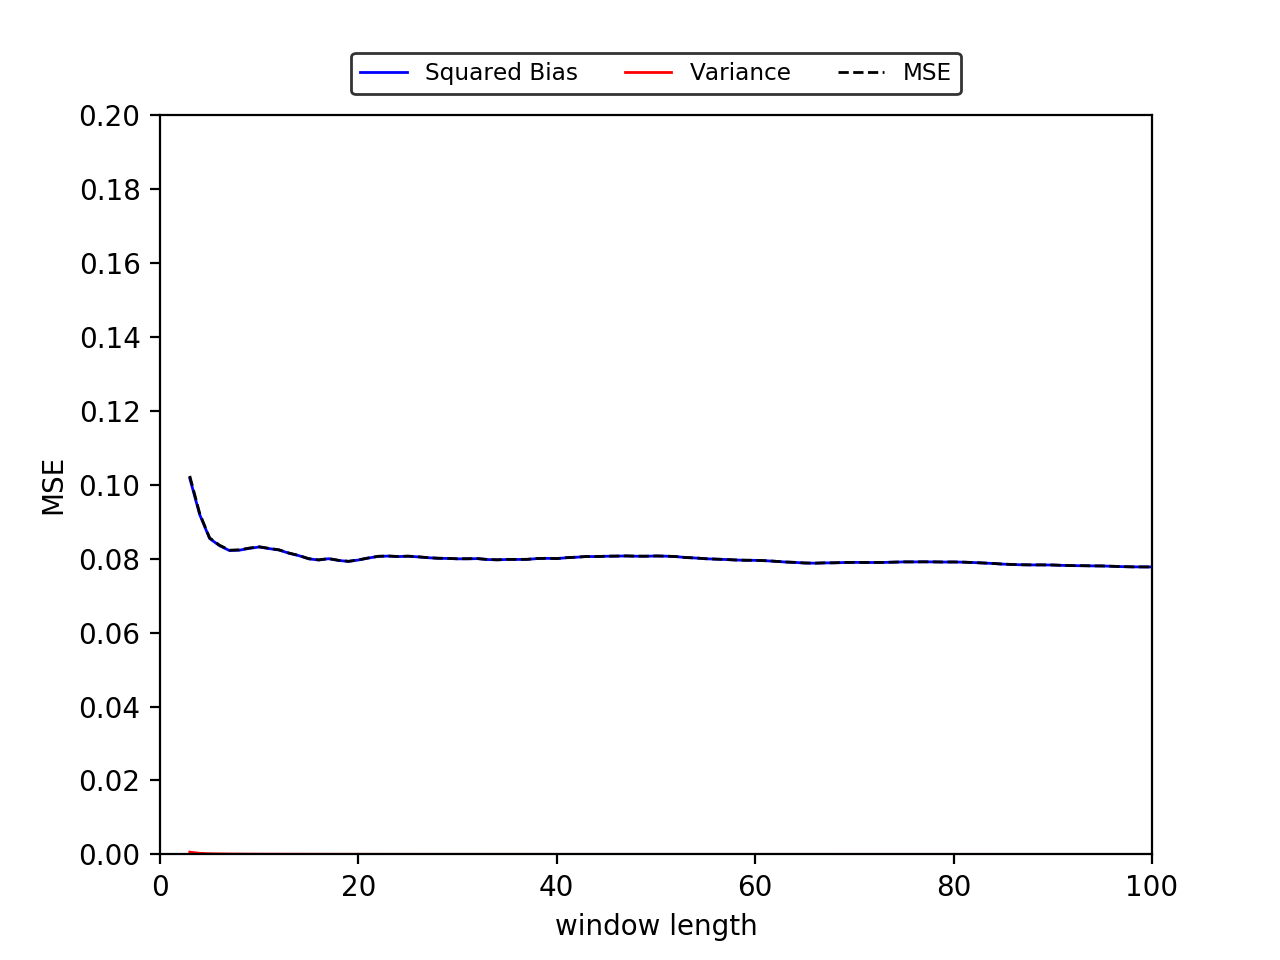
\includegraphics[width=\textwidth]{decom_mse_knn_IDW_pearson_proxy.png} 
		\caption{Bias-variance decomposition for KNN estimates constructed from inverse distance weighted averages and Pearson covariates.} 
		\label{fig:decom_mse_knn_IDW_pearson_proxy}
	\end{subfigure}
	\hfill  
	\begin{subfigure}[b]{0.49 \textwidth}
		\centering 
		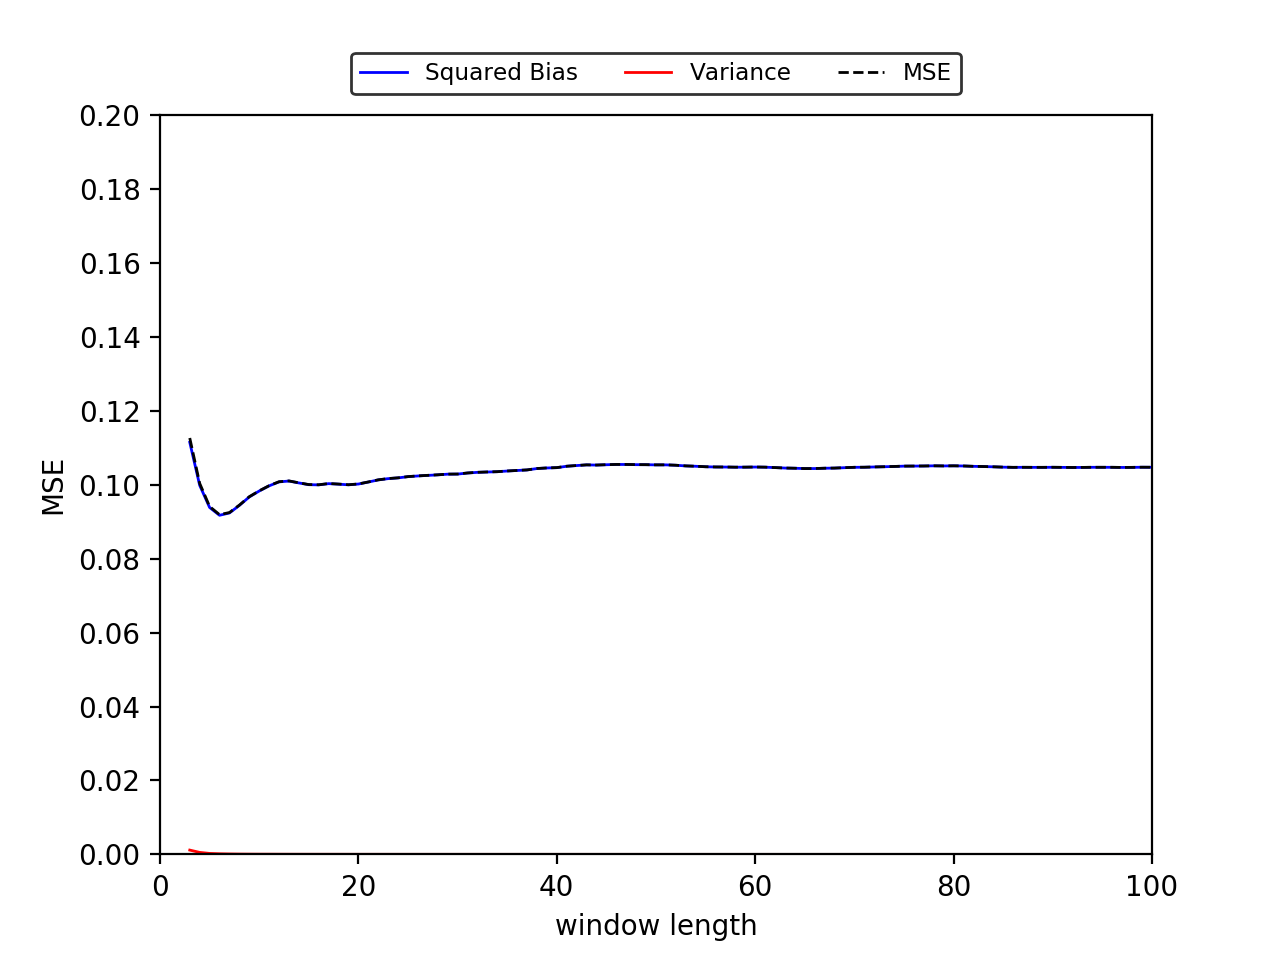
\includegraphics[width=\textwidth]{decom_mse_knn_IDW_kendall_proxy.png} 
		\caption{Bias-variance decomposition for KNN estimates constructed from inverse distance weighted averages and Kendall covariates.} 
		\label{fig:decom_mse_knn_IDW_kendall_proxy}
	\end{subfigure}
	\caption{MSE for KNN estimates with different weighting functions, Pearson and Kendall Moving Window bootstrap estimates as covariates and proxy correlation.}
	\label{fig:decom_mse_knn_len_train_IDW_pearson_kendall_proxy}
\end{figure}

\noindent
The accuracy of the two different parameterisations is compared by using mean squared error (MSE) between estimated and actual correlations. Regardless of the choice of window length, MSE from KNN with an uniform weighting function and the set of covariates and output variable constructed from Pearson and Kendall moving window estimates are approximately between 0.0774 and 0.0923, and 0.1054 and 0.1118, respectively. MSE from KNN with an inverse distance weighting function is approximately between 0.0778 and 0.1024, and between 0.0919 and 0.1127 when Pearson and Kendall moving window estimates are used as covariates and output variable, respectively. This implies that Pearson moving window estimates as covariates and approximation of true correlation in KNN seems more appropriate for the simulated data than Kendall moving window estimates, regardless of the weighting function; Fig. \ref{fig:decom_mse_knn_len_train_pearson_proxy} depicts a lower MSE for all window sizes compared with MSE in Fig. \ref{fig:decom_mse_knn_len_train_kendall_proxy} and Fig. \ref{fig:decom_mse_knn_IDW_pearson_proxy} depicts a lower MSE for all window sizes compared with MSE in Fig. \ref{fig:decom_mse_knn_IDW_kendall_proxy}. An explanation for this observation is given along the same lines as for Pearson and Kendall moving window estimates in Section \ref{sec:true_correlation}; the simulated asset returns follow a multivariate normal distribution, i.e. an elliptical distribution. Therefore, it makes sense that lower MSE values are obtained when true correlation in KNN is approximated using a linear correlation coefficient such as Pearson. Moreover, the choice for an inverse distance weighting function seems to have no performance advantage over an uniform weighting function in the case true correlation is approximated using moving window estimates. Interestingly, this is in contrast with results obtained from KNN estimates with true correlation in Section \ref{sec:knn_true_cor}. Finally, the variance of MSE from KNN with uniform weighting function and the set of covariates constructed from Pearson and Kendall moving window estimates are approximately 3.98e-6 and 9.26e-7, respectively. The variance of MSE from KNN with inverse distance weighting function and the set of covariates constructed from Pearson and Kendall moving window estimates are approximately 8.46e-6 and 8.61e-6, respectively. The difference in sensitivity to the choice of window length between the different parameterisations is negligible small if significant at all. \\

\noindent 
Similar to Section \ref{sec:knn_true_cor}, this section is concluded with a comparison of the function approximation capabilities of the KNN algorithm and Pearson and Kendall moving window estimates. The comparison is based on MSE between estimated and actual correlations. Fig. \ref{fig:mse_knn5_len_train_pearson_kendall_proxy} shows MSE from KNN with default parameterisation, i.e. number of neighbors equals 5, an alternative parameterisation with an uniform distance weighting function and the full training set used for estimating time-varying correlations. Additionally Pearson and Kendall moving window estimates of time-varying correlations are shown. According to MSE, parameterisations of the KNN algorithm with approximated covariates and output variable performs significantly better than those of Pearson and Kendall moving window estimates for small window sizes. Moreover, parameterisations of the KNN algorithm with an alternative distance weighting function and full use of training data set results in significantly smaller MSE compared to Pearson and Kendall moving window estimates for all window sizes. Thus, similar to the analysis in Section \ref{sec:knn_true_cor}, KNN estimates with an increase in the number of neighbors have lower MSE, particularly for smaller window sizes. This result follows from the fact that time-varying correlations are then estimated using increased sample information, which positively contributes to capturing time variation in correlations. Finally, the variance of MSE from KNN estimates with default parameterisation and with the combination of an uniform distance weighting function and use of full training set in Fig. \ref{fig:mse_knn5_len_train_pearson_kendall_proxy} are 5.70e-4 and 3.98e-6, respectively, while that of Pearson and Kendall moving window estimates are 0.0040 and 0.0037, respectively. In other words, the KNN algorithm with approximated covariates and output variable is significantly less sensitive to the choice of window length than Pearson and Kendall moving window estimates of correlation.  \\

\noindent
Concludingly, alternative parameterisations of the KNN algorithm with approximated covariates and output variable also satisfy the positive semi-definiteness condition in the time-varying correlation matrix $R_t$ for all time $t$ under all choices of window length in the interval 0 to 100. Fig. \ref{fig:det_knn_len_train_IDW_pearson_kendall_proxy} presents the obtained minimum determinants of $R_t$ for all choices of window length under the proposed alternative parameterisations.


\begin{figure}[H] 
	\centering
	\begin{subfigure}[b]{0.49 \textwidth}
		\centering 
		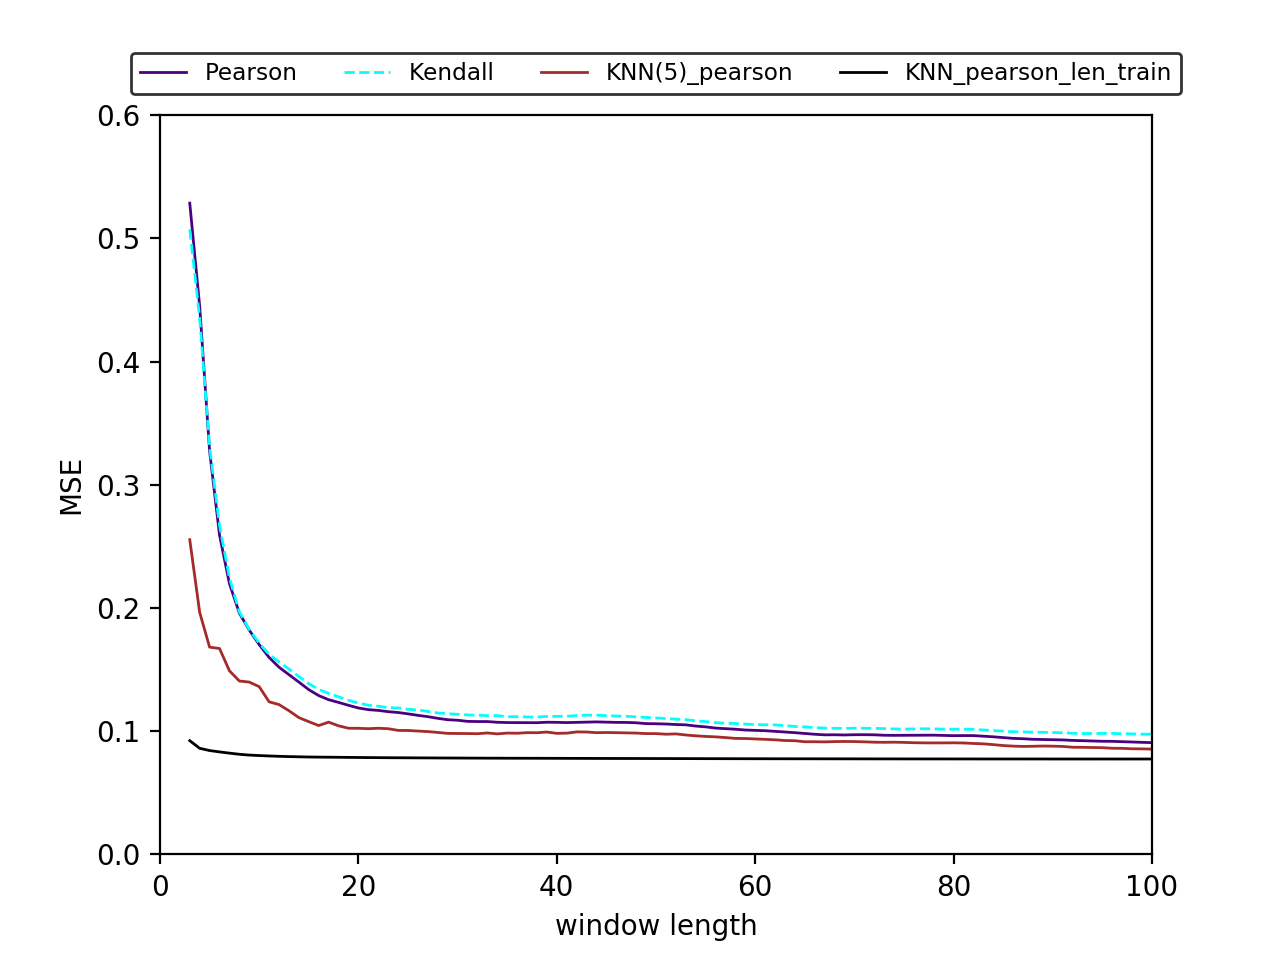
\includegraphics[width=\textwidth]{mse_knn5_len_train_pearson_kendall_proxy} 
		\caption{MSE for KNN with Pearson covariates and proxy correlation, Pearson and Kendall Moving Window bootstrap estimates.}
		\label{fig:mse_knn5_len_train_pearson_kendall_proxy}
	\end{subfigure}
	\hfill
	\begin{subfigure}[b]{0.49 \textwidth} 
		\centering
		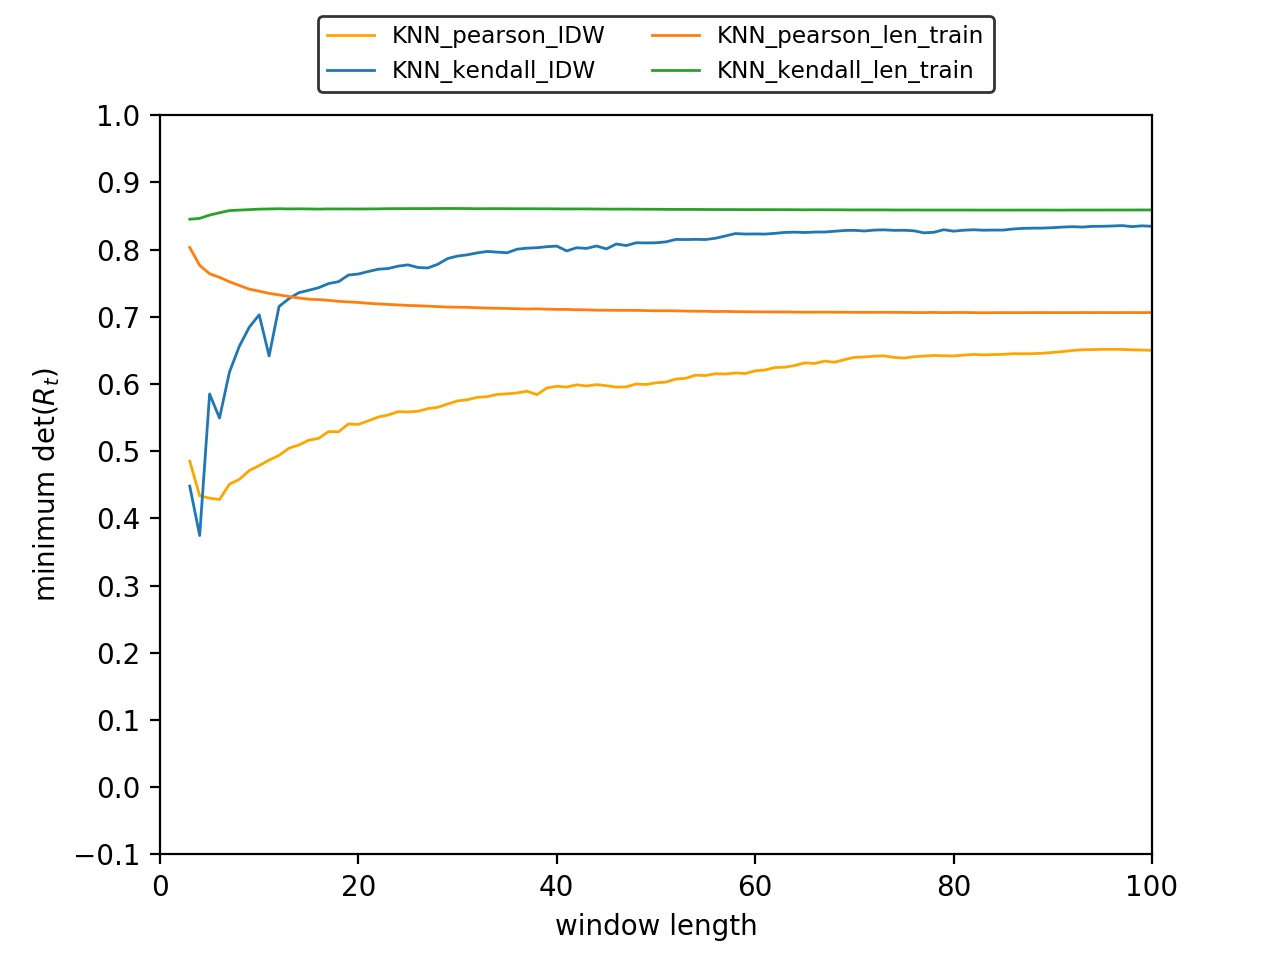
\includegraphics[width=\textwidth]{det_knn_IDW_len_train_pearson_kendall_proxy}
		\caption{Minimum determinants for KNN using uniform and inverse distance weighting function, Pearson and Kendall covariates and proxy correlation.}
		\label{fig:det_knn_len_train_IDW_pearson_kendall_proxy}
	\end{subfigure}	
	\caption{Comparison MSE and minimum determinants for KNN with Pearson covariates and proxy correlation, Pearson and Kendall Moving Window bootstrap estimates.}
	\label{mse_det_knn5_len_train_pearson_kendall_proxy}
\end{figure}







%%%%%%% RANDOM FOREST PROXY %%%%%%%%%%%%%%
\subsection{Random Forest} \label{sec:rf_proxy_cor}
In order to obtain time-varying correlations, $\rho_t$, with random forests algorithm, the set of covariates is defined by lagged Pearson and Kendall moving window estimates and minimum and maximum asset return values from the last period, denoted by $min_{i,j}(y_{i,j,t-1})$, and $max_{i,j}(y_{i,j,t-1})$, respectively.  \\

\noindent
The accuracy of RF estimates with Pearson and Kendall covariates for time-varying correlation is compared by using mean squared error (MSE) between estimated and actual correlations. MSE from RF with Pearson and Kendall moving window estimates of correlation for covariates and as output variable are shown in Fig. \ref{fig:mse_rf10_pearson_kendall_proxy}. Regardless of the choice of window length, MSE from RF with Pearson and Kendall covariates are between 0.0868 and 0.2318, and 0.0946 and 0.2321, respectively. The variance of MSE from RF estimates with Pearson covariates is approximately 4.54e-4 while that of RF estimates with Kendall covariates is approximately 3.23e-4. Interestingly, Fig. \ref{fig:mse_rf10_pearson_kendall_proxy} shows that MSE from RF estimation with Pearson or Kendall approximations for the output variable varies substantially for smaller window sizes. Although, less variation is observed when compared with MSE from Pearson and Kendall moving window estimates depicted in Fig. \ref{fig:mse_pearson_kendall_bootstrap}. This observation is analogous to the comparison of KNN estimates of correlation for both true correlation and approximated correlation as output variable. \\

\noindent
Moreover, RF estimates of time-varying correlation where both the set of covariates and output variable is constructed from Pearson and Kendall moving window estimates satisfy the positive semi-definiteness condition in the time-varying correlation matrix $R_t$ for all time $t$ under all considered choices of window length. Fig. \ref{fig:det_rf10_pearson_kendall_proxy} presents the obtained minimum determinants of $R_t$ for all choices of window length. Although the minimum determinants for smaller window sizes approach 0, they remain nonnegative for all time $t$.

\begin{figure}[H]
	\centering
	\begin{subfigure}[b]{0.49 \textwidth} 
		\centering
		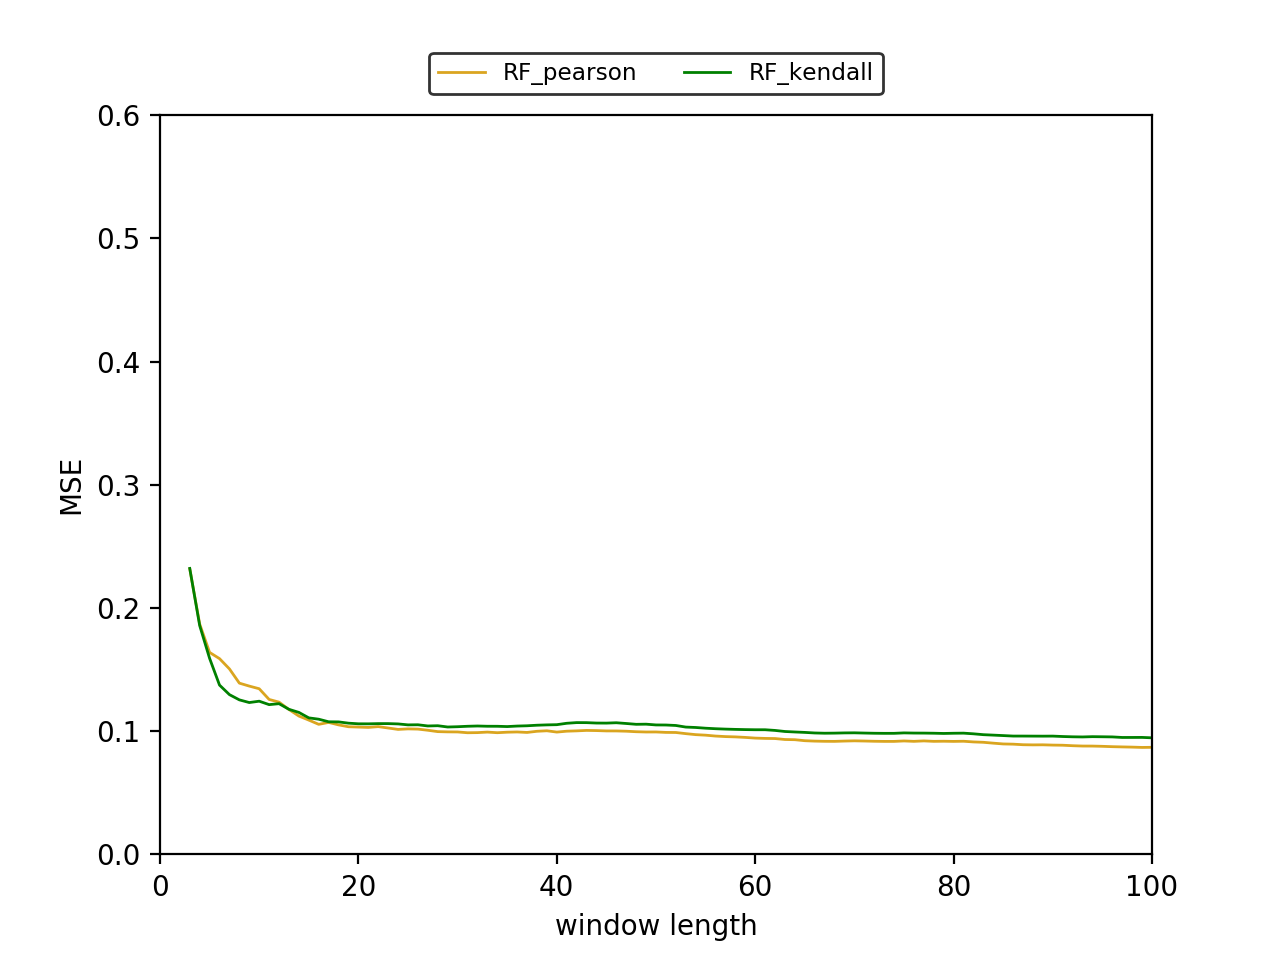
\includegraphics[width=\textwidth]{mse_rf10_pearson_kendall_proxy}
		\caption{MSE for RF with covariates from Pearson and Kendall and proxy correlation.}
		\label{fig:mse_rf10_pearson_kendall_proxy}
	\end{subfigure}
	\hfill
	\begin{subfigure}[b]{0.49 \textwidth} 
		\centering
		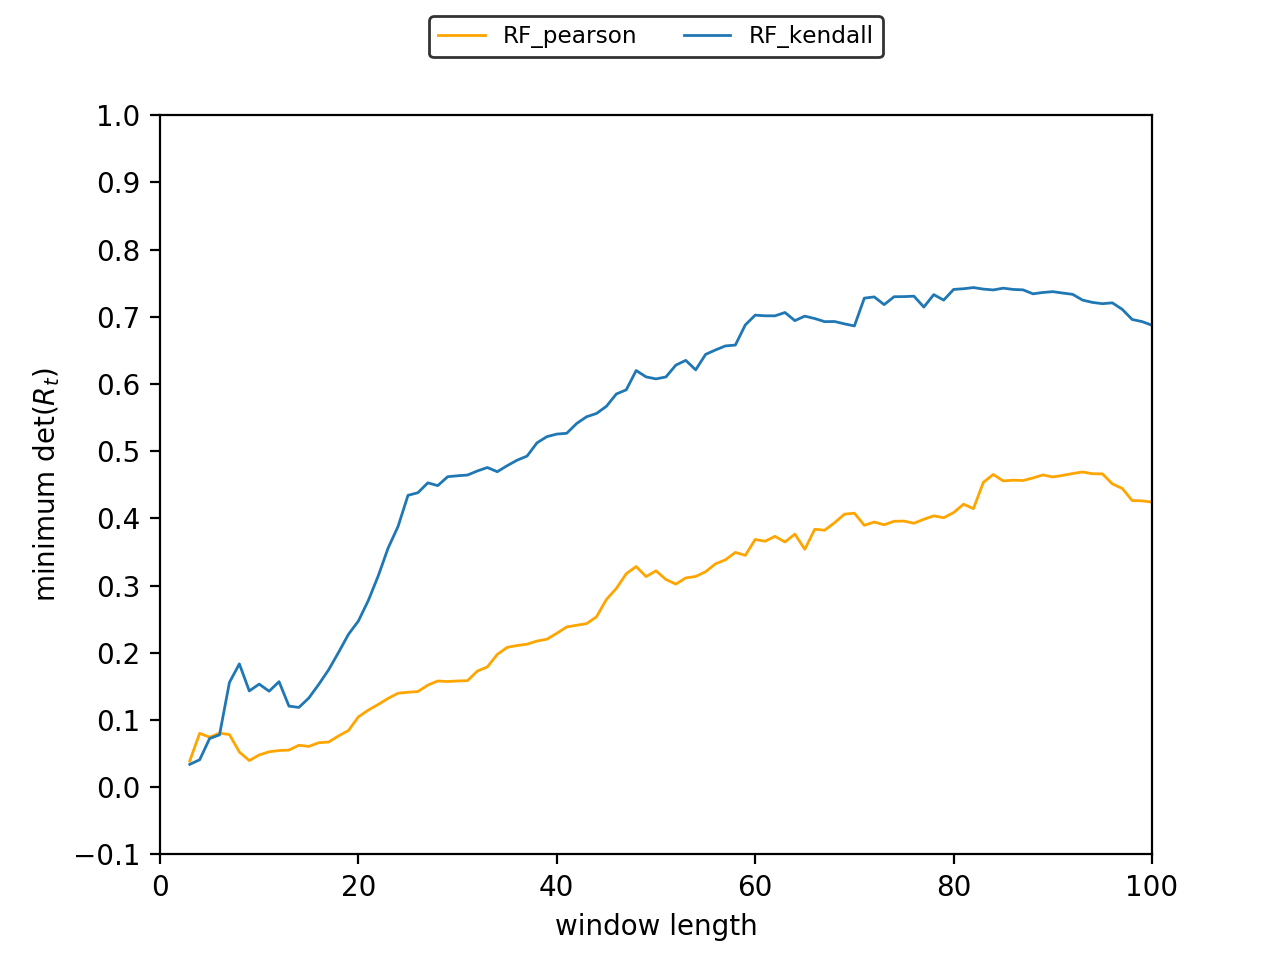
\includegraphics[width=\textwidth]{det_rf10_pearson_kendall_proxy}
		\caption{Minimum determinants for RF with covariates from Pearson and Kendall and proxy correlation.}
		\label{fig:det_rf10_pearson_kendall_proxy}
	\end{subfigure}
	\caption{Comparison MSE and minimum determinants for RF(n\_estimators=10) with covariates from Pearson and Kendall and proxy correlation.}
	\label{fig:mse_det_rf10_pearson_kendall_proxy}
\end{figure}

\noindent
A visual inspection of the plots in Fig. \ref{fig:rf_pearson21_bootstrap_proxy} and Fig. \ref{fig:rf_kendall21_bootstrap_proxy} results in an analysis that is analogous to the analysis of KNN estimates with approximations of correlation instead of actual correlation in Section \ref{sec:knn_proxy_cor}. It is clear that the uncertainty in the time-varying correlation $\rho_t$, which is illustrated by the 99\% confidence interval, is smaller for RF estimates compared to Pearson moving window estimates and Kendall moving window estimates, even though both the set of covariates and the output variable of the RF algorithm are based on approximations of correlation instead of actual correlation. These figures also show smaller uncertainty in the time-varying correlation $\rho_t$ when compared with RF estimates with true correlation as the output variable, which are depicted in Fig. \ref{fig:decom_mse_rf10_pearson_kendall_true}; RF estimates of correlation with true correlation as output variable in Fig. \ref{fig:rf_pearson21_bootstrap_true} and Fig. \ref{fig:rf_kendall21_bootstrap_true} are much more volatile. RF estimates with approximated correlation as output variable in Fig. \ref{fig:rf_pearson21_bootstrap_proxy} and Fig. \ref{fig:rf_kendall21_bootstrap_proxy} , however, follow the increases and decreases of the actual correlation smoother, with tighter confidence intervals. This is a more desirable result as it is not expected that correlation between assets changes that drastically at each time period. \\

\noindent
The MSE decompositions into bias and variance terms from RF estimates of correlation are shown in Fig. \ref{fig:rf_pearson21_bootstrap_proxy} and Fig. \ref{fig:decom_mse_rf10_pearson_proxy}. These figures indicate that the RF algorithm with approximated output is more sensitive to the choice of the window length for smaller window sizes compared to RF algorithm with true correlation depicted in Fig. \ref{fig:decom_mse_rf10_pearson_kendall_true}. This observation is similar to the observation when comparing the KNN algorithm with different outputs and can be explained by error propagation: the effect of covariates' uncertainties (or errors) on the error of the function based on them. In the case when the RF algorithm uses proxies for output variables, the error associated with approximation of true correlation using moving window estimates is propagated to the output of the RF algorithm. Fig. \ref{fig:decom_mse_rf10_pearson_proxy} and Fig. \ref{fig:decom_mse_rf10_kendall_proxy} show, however, that the RF algorithm with approximated output is considerably less sensitive to the choice of the window length for smaller window sizes when compared to Pearson and Kendall moving window estimates of correlation depicted in Fig. \ref{fig:decom_mse_pearson}  and Fig \ref{fig:decom_mse_kendall}, respectively. Thus, analogous to the KNN algorithm with approximated covariates and output variable, the RF algorithm seems to mitigate the error propagation to some extend for smaller window sizes. A lower bias compared to Pearson and Kendall moving window estimates of correlation implies random forests may be a more suitable model for modeling time-varying correlations. Additionally, lower variance is observed when compared with Pearson and Kendall moving window estimates of correlation. This may be accredited to the internal workings of the RF algorithm.       



\begin{figure}[H]  % [h] parameter makes sure figures are located at 'this' location.
	\centering
	\begin{subfigure}[b]{0.49 \textwidth} % sum of widths should be less than text width if all one the same line
		\centering 
		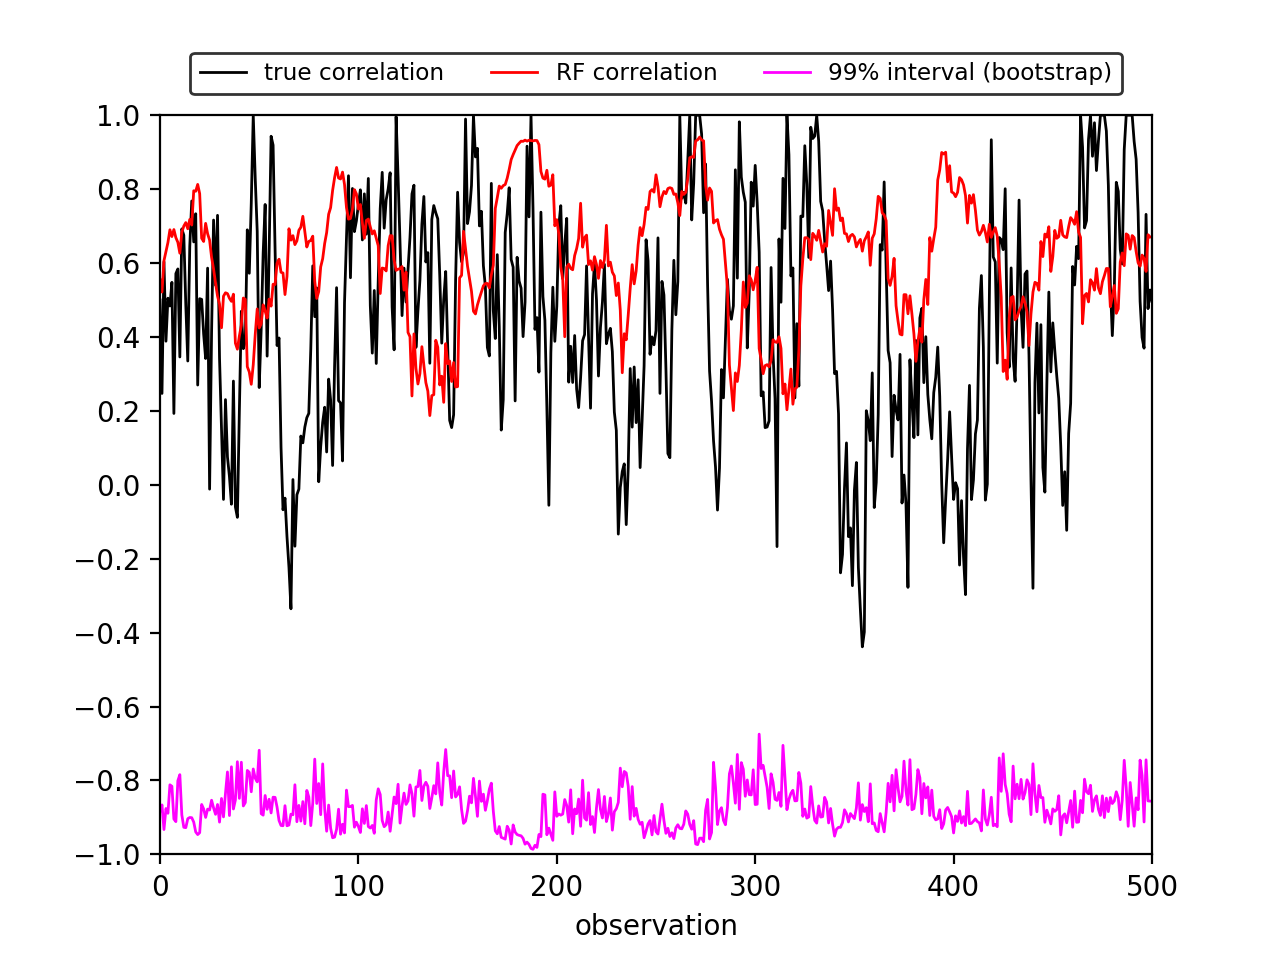
\includegraphics[width=\textwidth]{rf_pearson_21_estimates_bootstrap_proxy.png} 
		\caption{RF estimates with window size 21, Pearson as covariate and proxy correlation.} 	
		\label{fig:rf_pearson21_bootstrap_proxy}
	\end{subfigure} 
	\hfill	
	\begin{subfigure}[b]{0.49 \textwidth} 
		\centering 
		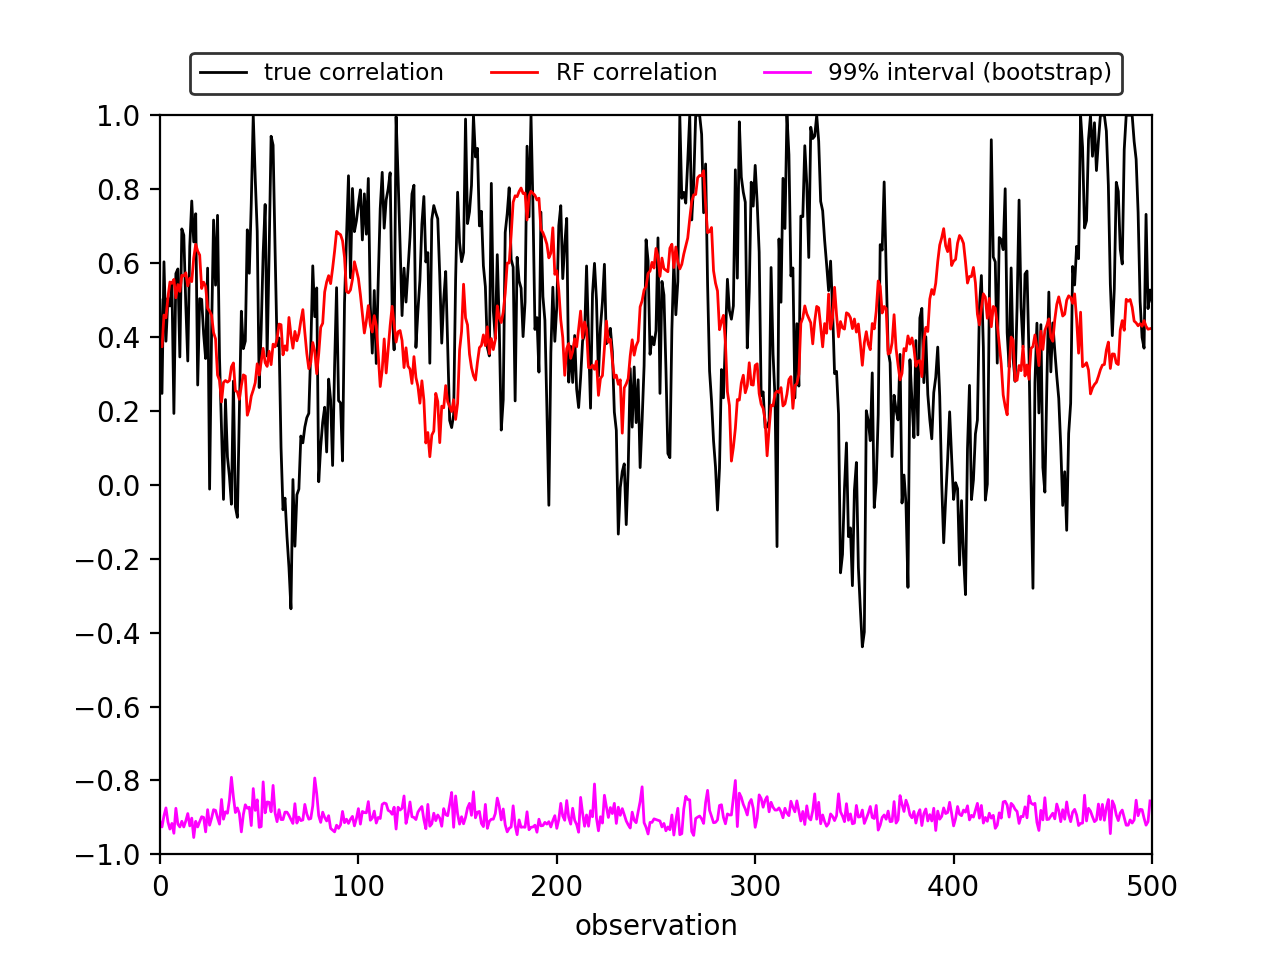
\includegraphics[width=\textwidth]{rf_kendall_21_estimates_bootstrap_proxy.png} 
		\caption{RF estimates with window size 21, Kendall as covariate and proxy correlation.} 
		\label{fig:rf_kendall21_bootstrap_proxy}
	\end{subfigure} 
	\hfill	
	\begin{subfigure}[b]{0.49 \textwidth}
		\centering 		
		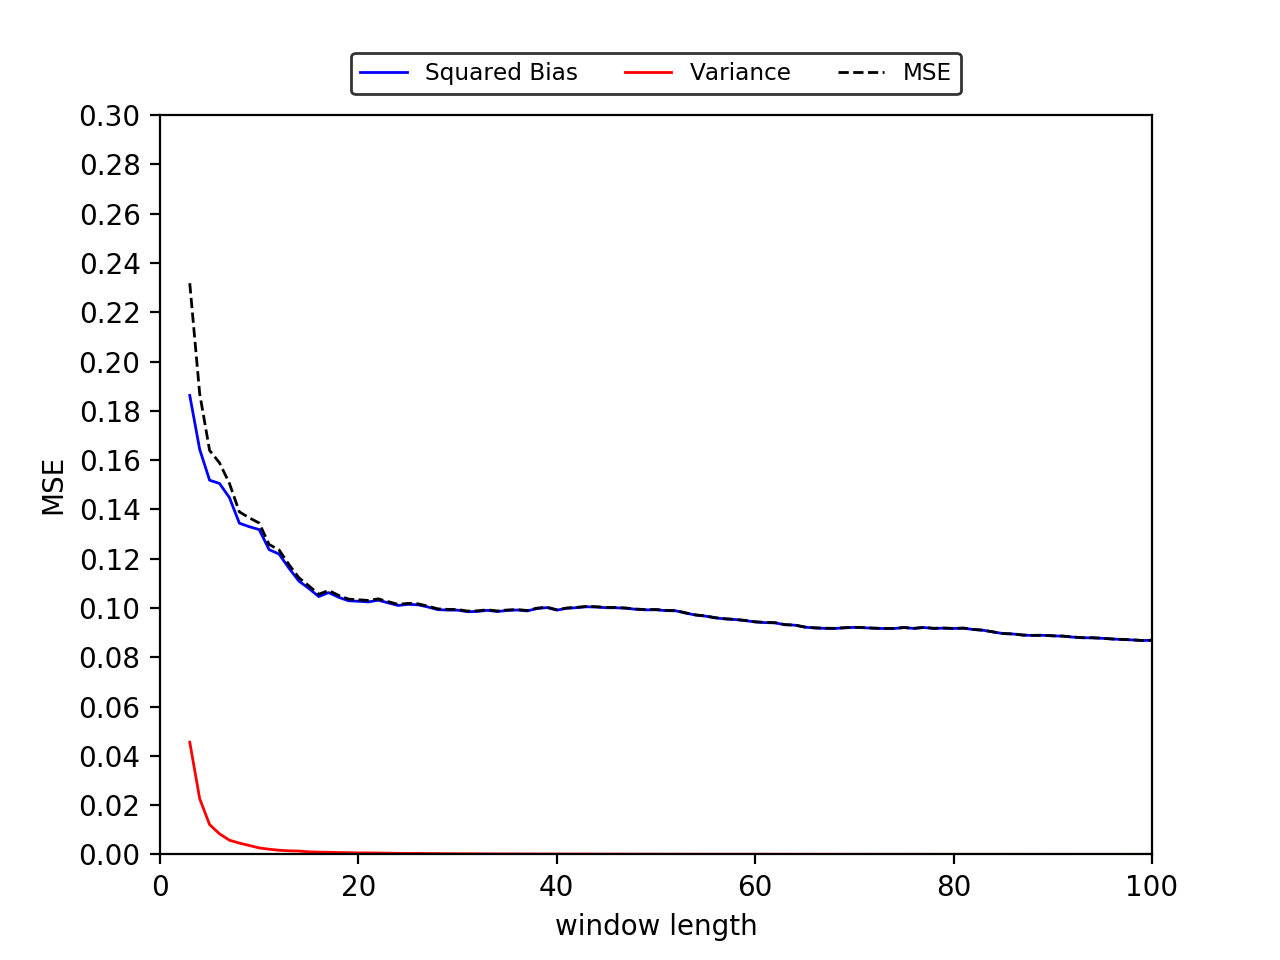
\includegraphics[width=\textwidth]{decom_mse_rf10_pearson_proxy.png} 
		\caption{Bias-variance decomposition for RF estimates with Pearson as covariate and proxy correlation.} 
		\label{fig:decom_mse_rf10_pearson_proxy}
	\end{subfigure}
	\hfill  
	\begin{subfigure}[b]{0.49 \textwidth}
		\centering 
		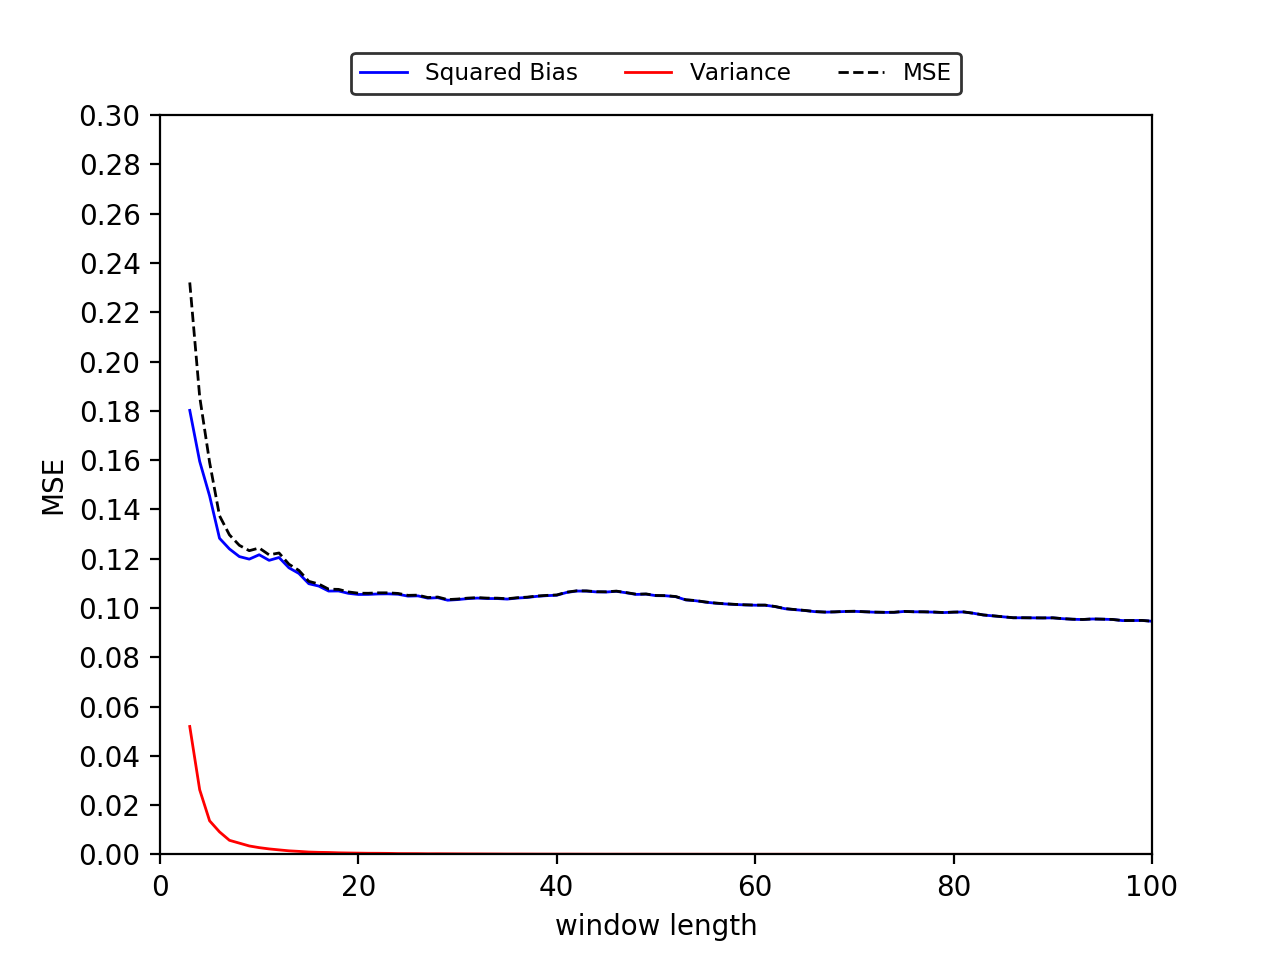
\includegraphics[width=\textwidth]{decom_mse_rf10_kendall_proxy.png} 
		\caption{Bias-variance decomposition for RF estimates with Kendall as covariate and proxy correlation.} 
		\label{fig:decom_mse_rf10_kendall_proxy}
	\end{subfigure}
	\caption{MSE for RF estimates with Pearson and Kendall Moving Window bootstrap estimates as covariates and proxy correlation.}
	\label{fig:decom_mse_rf10_pearson_kendall_proxy}
\end{figure}





\section{Conclusion simulation results}
\begin{enumerate}
	\item KNN with true correlation AND KNN with approximated output return positive semi-definite correlation matrices.
	\item KNN outperforms moving window estimates particularly for smaller window sizes but with full training set and potentially inverse distance weighting function for all window sizes in the interval [3, 100].
	\item MSE decomposition behavior KNN with true correlation exactly as expected/ predicted given MSE decomposition formulas. Except that with an increase in $k$, we initially observe improved squared bias.
	\item RF with true correlation AND RF with approximated output return positive semi-definite correlation matrices.
	\item RF exhibits higher bias than KNN. RF thus seems less appropriate model at this point. However, given the very small covariate dimension very little decorrelation of trees is possible which would results in variance reduction and possibly MSE reduction. Given higher dimensional covariate space in context of systems of correlations we continue to opt for RF estimation of time-varying correlations. 
	\item The difference in accuracy, measured by the MSE, between using Pearson and Kendall approximations of true correlation appear negligible small for the simulation study, regardless whether Nearest Neighbor or Random Forest algorithm was used.  
	\item Both KNN and RF estimates with approximated correlation as output variable follow the increases and decreases of the actual correlation smoother, with tighter confidence intervals in comparison to KNN and RF estimates with true correlation as the output variable. This is a more desirable result as it is not expected that correlation between assets changes that drastically at each time period. 
	\item One source of variance: noise in output and/or covariates as they are approximations. INSERT this somewhere in the analysis.
\end{enumerate}




%%%%%%%%%%%%%%%%%%%%%%%%%%%%%%%%%%%%%%%%%%%%%%%%%%%%%%%%%%%%%%
%%%%%%%%				      SYSTEMS OF CORRELATIONS							%%%%%%%%%
%%%%%%%%%%%%%%%%%%%%%%%%%%%%%%%%%%%%%%%%%%%%%%%%%%%%%%%%%%%%%%
\chapter{Systems of Correlations in Quantitative Financial Risk Management} \label{chap:multivariate_analysis}
The focus of this part of the analysis is modelling dependencies and  we continue to opt for correlation as a measure for dependency. However, the focus of analysis in a multivariate setting is a \textit{system of correlations} rather than \textit{individual correlations}. 


\bigskip
\noindent
\textbf{Question: Why model dependencies? Answer: In our work, we model dependencies for practical purposes such as to improve strategy for portfolio and risk management.} 

\bigskip
\noindent
We will now demonstrate the role of correlations in financial decision making. Specifically, we will establish some notation that is necessary to study the risk of portfolios consisting of an arbitrary number of assets, $k$. We will compare DCC with other time-varying correlation estimators, namely: knn and rf through the variance-covariance decomposition. 

\section{Value-at-Risk as Measure for Market Risk}
\textbf{Idea: VaR/ CVaR performance under normality assumption (backtesting strategies). It is ok to assume normality assumption solely for the purpose of comparing algorithms for correlation estimation. Moreover, major assumption VaR is that asset returns are multivariate Gaussian distributed.} \\

\begin{enumerate}
	\item Use decomposition of conditional variance-covariance matrix $H_t = D_t R_t D_t$
	\item $D_t$ is obtained by estimation of univariate conditional variances with GARCH(1,1) models 
	\item $R_t$ is obtained by estimation of correlations with learner models and DCC-GARCH (benchmark)
	\item Check semi positive-definiteness of obtained $H_t$ and use it for VaR computations and backtesting.
	\item Backtesting periods in tranquil times and in volatile times
\end{enumerate}

\noindent
Following is a nice empirical study of VaR estimation just like we want to do here. \\
\noindent
https://www.tandfonline.com/doi/full/10.1080/1331677X.2017.1305773 \\

\noindent
For analysis of the conditional correlations forecasting accuracy implied by different conditional volatility models, the one-day-ahead out-of-sample Value-at-Risk (henceforth VaR) is computed and a backtesting analysis is performed. The idea is to take $k$ assets, estimate the model parameters using a training set and apply the proposed models to obtain out-of-sample one-step-ahead forecasts of the conditional variance-covariance matrix of all assets, $H_t$, where conditional correlation matrix $R_t$ is estimated through learner models and benchmark DCC-GARCH. Then it is possible to compute one-day-ahead out-of-sample VaR and perform a backtesting analysis.  \\

\noindent
One definition of VaR is the maximum loss which is not exceeded at a given confidence level $\alpha$. A more formal definition in terms of the $\alpha$-quantile of the loss distribution is given by: \\

\begin{mydef}[\cite{ref:QRM2015} \textbf{Value-at-Risk}] \label{def:VaR}	
	\begin{equation}
		VaR_{\alpha} = inf\{l \in \mathbb{R}:P(L>l) \le 1-\alpha\}=inf\{l \in \mathbb{R}: F_L(l) \ge \alpha\}.
	\end{equation}
	where $F_L(l) = P(L \le l)$ denotes the distribution function  of the corresponding loss distribution.
\end{mydef}

\noindent
In other words: VaR is the loss value for which the probability of observing a larger loss is equal to $1-\alpha$ \citep{ref:Cirillo2016}. \\



\noindent
VaR is determined after definition of the portfolio return distribution, where portfolio return $p_t = w' y_t + a_t$. It is noted that the validation of the portfolio risk using backtesting measures is not straightforward without further assumptions on $a_t$: The mean-corrected log returns $a_t$ are assumed to be multivariate Gaussian, i.e. $a_t \sim \mathcal{N}(0, H_t)$. The first two moments of the portfolio return are then given by:

\begin{align}
	\mathbb{E}[p_t] &= \mu_{p,t} =  w' \mathbb{E}[\mu_t] \\
	Var[p_t] &= \sigma_{p,t}^2 =  w'H_tw 
\end{align}

\noindent
Consequently, the portfolio return distribution is given by:

\begin{align}
	p_t \sim \mathcal{N}(w' \mathbb{E}[\mu_t], w'H_tw)  \nonumber
\end{align}

\noindent 
If the conditional distribution of each asset return is assumed Gaussian, then the portfolio return also follows a Gaussian distribution as the multivariate Gaussian distribution is closed under linear transformations. The portfolio VaR for one day horizon at $\alpha$ confidence level is given by: 

\begin{align}
	VaR_{\alpha}(p_t) = \mu_{p,t} + \sigma_{p,t}z_\alpha 
\end{align}

\noindent 
where $z_\alpha$ is the critical value of the corresponding quantile $\alpha$. In our backtesting analysis, we compute a 95\% VaR such that $z_\alpha = 1.65$ under normality assumption. For simplicity, the sample mean is used as the mean equation and the proposed multivariate volatility model is applied to the mean-corrected data, i.e. $\mu_{p,t}$ is assumed constant. Furthermore, an equally weighted portfolio is used in our analysis as a number of papers \citep{ref:Plyakha2012} suggest that equally weighted portfolio strategies consistently outperform other optimization strategies. Moreover, the focus in this part of our analysis is on the evaluation of different models for conditional correlation forecasting instead of finding optimal portfolio weights and/or risk minimization.    


\section{Dynamic Conditional Correlation Model}
A multivariate extension of univariate GARCH modeling is the dynamic conditional correlation (DCC)  model which can be used for estimation of the conditional covariance matrix. The DCC model captures the advantages of GARCH models and simplifies the computation of multivariate GARCH models such as VEC-GARCH and BEKK. In the DCC model, time series of daily log returns on k assets $y_t$ is conditionally multivariate normal with mean zero. That is,

\begin{align}
	y_t &= H_t^{\frac{1}{2}}z_t \\
	H_t &= D_t R_t D_t \\
	D_t &= diag(\sigma_{11,t}, \dots, \sigma_{kk,t})
\end{align}

\noindent
where $H_t$ is the conditional covariance matrix and $R_t$ is the conditional correlation matrix. $D_t$ is a diagonal matrix with $\sigma_{11,t}, \dots, \sigma_{kk,t}$ on the main diagonal, which can be estimated through univariate GARCH models. \\


\noindent
\cite{ref:Engle2002} noted that $R_t$ is also the conditional covariance matrix of the standardized residuals, where the standardized residuals $\epsilon_t$ is defined as 

\begin{align}
	\epsilon_t = D_t^{-1}H_t^{\frac{1}{2}}z_t  \;\;\;  \sim \mathcal{N}(0, R_t)
\end{align}

\noindent
The DCC-GARCH(1,1) model as introduced by \cite{ref:Engle2002} is considered in this paper. This means that the the conditional correlations and the conditional variances are modelled by GARCH models. The first step is to estimate the univariate conditional variances with GARCH(1,1) model for obtaining $D_t$. Estimation of the parameters in the GARCH model  can be done by maximum likelihood. The second step is to estimate the conditional correlation matrix $R_t$. In this paper, the DCC-GARCH(1,1) model is considered and reparameterisation of $R_t$ ensures both requirements for $R_t$ are satisfied:

\begin{align}
	R_t &= \dot{Q}_t^{-1} Q_t \dot{Q}_t^{-1} \\
	Q_t &= (1-\alpha_0-\beta_0) \bar{Q} + \alpha_0 \epsilon_{t-1} \epsilon'_{t-1} + \beta_0 Q_{t-1} \label{eq:DCC(1,1)-GARCH}
\end{align}

\noindent
where $Q_t$ is a positive semi-definite matrix defining the structure of the correlation dynamics and $\bar{Q} = Cov(\epsilon_t \epsilon'_t) = \mathbb{E}[\epsilon_t \epsilon'_t]$ is the unconditional covariance matrix\footnote{$\bar{Q}$ can be thought of as representing the long-run correlation structure.} of the standardized residuals $\epsilon_t$, which can be estimated by

\begin{align}
	\bar{Q}_t = \frac{1}{T} \sum_{t=1}^T \epsilon_t \epsilon'_t
\end{align}

\noindent
where $\dot{Q}_t$ is a diagonal matrix with the square root of the diagonal elements of $Q_t$ at its diagonal. $\dot{Q}_t$ rescales $Q_t$ to ensure the requirement that the absolute value of all elements in the conditional correlation matrix $R_t$ is equal or less than one. In order for $Q_t$ to satisfy the condition of a positive semi-definite matrix (and hence guarantee positive semi-definiteness for $H_t$ under condition that $D_t$ is also positive semi-definite), the scalars $\alpha_0$ and $\beta_0$ must satisfy:

\begin{align}
	\alpha_0 \ge 0, \; \beta_0 \ge 0 \;\;\;\; \text{and} \;\;\;\; \alpha_0 + \beta_0 < 1 \nonumber
\end{align} 

\noindent
"Engel (2002) performed a comparison of several conditional covariance and showed
that DCC-GARCH model was overall best in estimation. Despite its accurate
estimation of future covariances, potential weaknesses still exist. One potential
drawback of the DCC-GARCH model is that all conditional correlations follow
the same dynamic structure is unrealistic in practice./  However, an unrealistic assumption of one parameter governing all correlation dynamics underlies the DCC model. " With using machine learning models we drop this restriction. 

\section{Univariate GARCH(1,1)}
\begin{align}
	\sigma^2_t = \omega + \alpha_1*\epsilon_{t-1} + \beta_1*\sigma^2_{t-1}    
\end{align}

\noindent
where the unconditional variance equals $\frac{\omega}{(1-\alpha_1-\beta_1)}$ 

\section{Backtesting methodology}
Backtesting is the process of verifying whether one's model performs adequately. In this work, the goal of a backtesting procedure is to statistically compare the models used for estimating time-varying correlations. \cite{ref:Christoffersen1998} defined two properties that must both be satisfied by a valid VaR model: unconditional coverage property and independence property. Two statistical tests are considered in this work for the assessment of these two properties: a failure test of unconditional coverage using the Kupiec test \citep{ref:Kupiec1995} and an independence test using Christoffersen's Markov test \citep{ref:Christoffersen1998}. All test results are provided given a confidence level of 0.95. The test confidence level may be different from the considered quantiles of the loss distribution and the reader is advised not to interchange them. \\

\noindent
\cite{ref:Kupiec1995} developed a statistical test to asses the unconditional coverage of a VaR model; the hypothesis that the the total number of exceedances equals the expected number of exceedances, given the independence property is satisfied. 
\cite{ref:Kupiec1995} tests for unconditional coverage through formulation of a log-likelihood ratio, that is,

\begin{align} \label{eq:Kupiec_test}
	LR_{uc} = 2 \ \text{ln} \Bigg( \bigg(\frac{1-I(\alpha) / T}{1-\alpha}\bigg)^{T-I(\alpha)} \bigg(\frac{I(\alpha) / T}{\alpha} \bigg)^{I(\alpha)}\Bigg)
\end{align}

\noindent
In Eq. \ref{eq:Kupiec_test}, $T$ is the number of observations and $I(\alpha)$ is the total number of exceedances. An exceedance $I_t(\alpha)$ is defined as $r_{t+1} < VaR_t(\alpha)$. The test statistic is asymptotically distributed as a chi-square distribution with 1 degree of freedom under the null hypothesis that the VaR model is adequate, i.e. the VaR model produces an expected proportion of exceedances equal to $\alpha$. Moreover, as the Kupiec test statistic is two sided, the model under consideration is rejected in the following two cases: there are too few exceedances, i.e. the model is excessively conservative, or there are too many exceedances, i.e. an underestimation of risk.   \\

\noindent
An important shortcoming of Kupiec's test is that it solely examines the frequency of exceedances but neglects to assess any form of independence in the occurrence of exceedances. As a consequence, the test may fail to reject a model producing clustered VaR exceedances. This is problematic because, in theory, one would expect exceedances to be evenly spread over time. A clustering of exceedances implies the independence property is violated as an adequate VaR model should exhibit responsiveness to changing market conditions, e.g. changes in volatility and correlations, thereby making clustered exceedances less likely. Exceedance clustering is an important concept as consecutive unexpected losses may be more stressful to an institution compared to unexpected losses occurring somewhat more frequently than expected but are evenly spread out over time  \citep{ref:Campbell2005}. Christoffersen's Markov test \citep{ref:Christoffersen1998} is one of a variety of tests that explicitly examines the independency property of VaR exceedances. The Markov test examines whether the likelihood of a VaR exceedance depends on whether a VaR exceedance occurred on the previous day. Under the null hypothesis, the probability of an exceedance proceeded by a non-exceedance equals the probability of an exceedance proceeded by an exceedance, i.e. $\pi_{01} = \pi_{11}$ in Eq. \ref{eq:Christoffersen_test}. In other words, the probability of exceeding today's VaR should be independent of whether yesterday's VaR was exceeded or not. Only then the VaR measure accurately reflects the underlying portfolio risk \citep{ref:Campbell2005}. \cite{ref:Christoffersen1998} observed that testing for independence can be formulated as a log-likelihood ratio test, that is, 

\begin{align} \label{eq:Christoffersen_test}
	LR_{ind} = -2 \ \text{ln} \Bigg(\frac{(1-\pi_2)^{(n_{00}+n_{10})}\pi_2^{(n_{01}+n_{11})}}{(1-\pi_{01})^{n_{00}}\pi_{01}^{n_{01}}(1-\pi_{11})^{n_{10}}\pi_{11}{^{n_{11}}}} \Bigg)
\end{align}

\noindent
where $n_{ij}$ is the number of transitions from $i$ to $j$ in the hit function series $I_t$, with $i,j \in \{0,1\}$, corresponding to non-exceedances and exceedances. The transition probability $\pi_{ij} = n_{ij} / \sum_j n_{ij} $ and $\hat{\pi}_2 = (n_{01}+n_{11}) / (n_{00}+n_{10}+n_{01}+n_{11})$. Moreover, the test statistic is asymptotically distributed as chi-square distribution with 1 degree if freedom assuming the null hypothesis. \\

\noindent
The main assumption underlying Christoffersen's Markov test is that the indicator function sequence of exceedances and non-exceedances satisfies the Markov property. However, \cite{ref:Christoffersen1998} only considers first order dependence, through a first-order Markov chain model, and this is considered a weakness of the independence test.   \\






\section{Data and descriptive statistics}
The raw dataset comprises 30 univariate time series of the log returns from the 30 Dow Jones Industrial Average index constituents. The raw log return series   


The raw price series is
cleaned by aligning and removing abnormalities: we manually
aligned the mismatched part and interpolated the missing
value by stochastic regression imputation (Little and Rubin
2014) where the imputed value is drawn from a Gaussian
distribution with mean and variance calculated by regression
on the empirical value within a short interval of 20 recent
days. The series is then transformed from actual prices st
into log-returns xt = log(st/st?1) and normalised. Moreover,
we combinatorically choose a predefined number d out
of 162 univariate log-return series and aggregate the selected
series at each time step to form a d-dimensional multivariate
time series, the choice of d is in accordance with the rank of
correlation, e.g. d = 6 in our experiments. Specifically, the actual dataset for training and evaluation comprises a collection of 2000 series of d-dimensional normalised
log-return vectors of length 2570 (approx. 7 years) with no missing values. We divide the whole dataset into two subsets for training and testing along the time axis: the first 2000
time steps of each series have been used as training samples whereas the rest 570 steps of each series as the test samples. \\

\begin{table}[H]
\centering
\captionsetup[subtable]{position=below}
\begin{tabular}{l c c c c c c}
\toprule
\multicolumn{1}{ c }{\textbf{Asset}} &
\multicolumn{1}{ r }{\textbf{Mean}} &
\multicolumn{1}{ r }{\textbf{St. error}} &
\multicolumn{1}{ r }{\textbf{Skewness}} &
\multicolumn{1}{ r }{\textbf{Ex. kurtosis}} &
\multicolumn{1}{ r }{\textbf{Minimum}} &
\multicolumn{1}{ r }{\textbf{Maximum}}  \\
\midrule 
AA    & 0.1127 & 0.0573    & 0.5472   & 3.07            & -10.30  & 13.13   \\
AXP   & 0.1423 & 0.0584    & 0.1443   & 2.82            & -11.48  & 12.02   \\
BA    & 0.0502 & 0.0578    & -0.6100  & 9.70            & -18.11  & 11.00   \\
BAC   & 0.0744 & 0.0573    & -0.2343  & 2.38            & -11.52  & 8.42    \\
C     & 0.1670 & 0.0662    & 0.2679   & 3.77            & -11.52  & 16.85   \\
CAT   & 0.0508 & 0.0618    & -0.1847  & 3.55            & -13.00  & 10.32   \\
CVX   & 0.0654 & 0.0440    & 0.1459   & 0.74            & -6.80   & 6.33    \\
DD    & 0.0773 & 0.0533    & -0.1229  & 1.76            & -9.54   & 7.08    \\
DIS   & 0.0541 & 0.0525    & -0.0653  & 3.19            & -10.96  & 10.13   \\
GE    & 0.1501 & 0.0443    & 0.0221   & 1.57            & -7.09   & 7.61    \\
GM    & 0.0742 & 0.0510    & 0.2079   & 0.73            & -6.54   & 7.23    \\
HD    & 0.1524 & 0.0563    & -0.0185  & 1.89            & -10.68  & 8.45    \\
HPQ   & 0.1237 & 0.0723    & -0.1391  & 3.66            & -14.91  & 15.20   \\
IBM   & 0.1433 & 0.0593    & -0.0094  & 6.07            & -16.20  & 12.36   \\
INTC  & 0.1854 & 0.0710    & -0.1340  & 1.83            & -13.45  & 12.87   \\
JNJ   & 0.1027 & 0.0447    & 0.1587   & 1.06            & -7.23   & 6.97    \\
JPM   & 0.1258 & 0.0603    & 0.1285   & 2.86            & -10.80  & 11.99   \\
AIG   & 0.1230 & 0.0493    & 0.2878   & 2.32            & -7.81   & 10.48   \\
KO    & 0.0688 & 0.0473    & -0.1593  & 3.38            & -11.09  & 8.02    \\
MCD   & 0.0827 & 0.0474    & 0.2760   & 3.54            & -10.61  & 10.31   \\
MMM   & 0.0616 & 0.0451    & -0.1907  & 2.46            & -10.07  & 5.91    \\
MRK   & 0.1073 & 0.0495    & -0.3158  & 2.44            & -9.40   & 8.05    \\
MSFT  & 0.2158 & 0.0617    & 0.0964   & 0.86            & -9.28   & 9.43    \\
PFE   & 0.1334 & 0.0572    & -0.0738  & 1.47            & -10.68  & 9.25    \\
PG    & 0.1064 & 0.0466    & -0.1860  & 1.90            & -10.23  & 6.55    \\
T     & 0.0809 & 0.0497    & -0.0333  & 1.65            & -8.80   & 7.96    \\
UTX   & 0.1194 & 0.0461    & -0.0767  & 1.41            & -7.88   & 5.61    \\
VZ    & 0.0865 & 0.0487    & 0.1218   & 1.82            & -7.53   & 8.54    \\
WMT   & 0.1509 & 0.0568    & -0.0164  & 1.63            & -10.22  & 7.64    \\
XOM   & 0.0895 & 0.0413    & 0.0075   & 1.11            & -7.69   & 5.75  \\ [1ex]
\bottomrule  
\end{tabular}
\caption[Descriptive statistics of Dow Jones Industrial Average daily log returns under tranquil conditions.]{Descriptive statistics of Dow Jones Industrial Average daily log returns under tranquil market conditions. Tick symbol is used to denote the company. Log returns are in percentages and the sample period is from January 1995 to December 1999 for 1253 observations.} 
\label{tab:stats_data_tranquil}
\end{table}

" It illustrates that the distribution
is clearly not symmetric. In fact it has a very noticeable
negative skew (i.e. leans to the right) as well as excess kurtosis
(i.e. is more peaked than a normal distribution; it has a kurtosis
value of 4.15, which is above the ?normal? value of 3.0). " \\

\noindent
The standard normal distribution has a kurtosis of zero. In addition, positive kurtosis indicates a fat-tailed distribution and negative kurtosis indicates a "light tailed" distribution. As we can see from table 5.1, the log return series from all DJI constituents exhibit positive excess kurtosis indicating the presence of fat left tails (cq. fat right tails in loss distribution), which was to be expected given the large body of empirical work on asset return distributions. This gives evidence to model the marginal innovation dynamics with Student-t distribution or even skewed student-t distribution. \\

\noindent
"The skewness for a normal distribution is zero, and any symmetric data should have a skewness near zero. Negative values for the skewness indicate data that are skewed left and positive values for the skewness indicate data that are skewed right. By skewed left, we mean that the left tail is long relative to the right tail. Similarly, skewed right means that the right tail is long relative to the left tail. If the data are multi-modal, then this may affect the sign of the skewness."



\begin{table}[H]
\centering
\captionsetup[subtable]{position=below}
\begin{tabular}{l c c c c c c}
\toprule
\multicolumn{1}{ c }{\textbf{Asset}} &
\multicolumn{1}{ r }{\textbf{Mean}} &
\multicolumn{1}{ r }{\textbf{St. error}} &
\multicolumn{1}{ r }{\textbf{Skewness}} &
\multicolumn{1}{ r }{\textbf{Ex. kurtosis}} &
\multicolumn{1}{ r }{\textbf{Minimum}} &
\multicolumn{1}{ r }{\textbf{Maximum}}  \\
\midrule 
AA    & -0.0879 & 0.0789    & -0.1156  & 12.28           & -17.50  & 20.87   \\
AXP   & -0.0612 & 0.0663    & -0.6442  & 13.31           & -19.34  & 16.51   \\
BA    & 0.0078  & 0.0508    & 0.3135   & 7.33            & -8.04   & 14.40   \\
BAC   & -0.0634 & 0.0836    & -0.6485  & 27.72           & -30.41  & 24.14   \\
C     & -0.1404 & 0.0951    & 0.7485   & 44.57           & -30.56  & 45.73   \\
CAT   & 0.0136  & 0.0570    & -0.5267  & 8.67            & -15.68  & 13.74   \\
CVX   & 0.0549  & 0.0550    & 0.2099   & 15.92           & -13.33  & 18.95   \\
DD    & -0.0337 & 0.0479    & -0.6138  & 10.44           & -12.03  & 10.87   \\
DIS   & 0.0021  & 0.0510    & 0.6270   & 12.55           & -10.24  & 14.83   \\
GE    & -0.0386 & 0.0507    & -0.5399  & 15.05           & -13.68  & 12.76   \\
GM    & -0.2079 & 0.1098    & -0.4240  & 17.59           & -37.27  & 30.09   \\
HD    & -0.0265 & 0.0533    & 0.5288   & 5.56            & -8.58   & 13.15   \\
HPQ   & 0.0405  & 0.0547    & 0.4409   & 8.66            & -14.08  & 13.56   \\
IBM   & -0.0028 & 0.0394    & -0.2946  & 5.44            & -8.65   & 9.13    \\
INTC  & -0.0553 & 0.0593    & -0.4881  & 5.55            & -13.24  & 11.17   \\
JNJ   & 0.0209  & 0.0312    & 0.9525   & 17.17           & -7.97   & 11.53   \\
JPM   & 0.0014  & 0.0734    & 0.0105   & 15.21           & -19.70  & 19.38   \\
AIG   & -0.2930 & 0.1435    & -6.7438  & 116.70          & -93.63  & 35.85   \\
KO    & 0.0012  & 0.0354    & 0.6094   & 18.26           & -9.08   & 12.99   \\
MCD   & 0.0822  & 0.0414    & 0.1701   & 3.79            & -8.31   & 8.98    \\
MMM   & -0.0219 & 0.0407    & -0.3889  & 8.36            & -9.38   & 9.43    \\
MRK   & -0.0172 & 0.0595    & -3.1433  & 45.14           & -31.19  & 12.25   \\
MSFT  & -0.0137 & 0.0488    & 0.4857   & 14.42           & -12.08  & 17.05   \\
PFE   & -0.0392 & 0.0452    & -0.4733  & 9.35            & -11.83  & 9.67    \\
PG    & 0.0252  & 0.0332    & -0.0734  & 9.61            & -8.23   & 9.73    \\
T     & 0.0257  & 0.0459    & 0.7294   & 11.60           & -8.04   & 15.05   \\
UTX   & 0.0166  & 0.0444    & 0.5550   & 9.82            & -7.26   & 12.79   \\
VZ    & 0.0184  & 0.0435    & 0.5097   & 9.75            & -8.42   & 13.65   \\
WMT   & 0.0102  & 0.0381    & 0.4087   & 7.29            & -8.42   & 10.49   \\
XOM   & 0.0608  & 0.0524    & 0.0570   & 14.47           & -15.04  & 15.87   \\ [1ex]
\bottomrule  
\end{tabular}
\caption[Descriptive statistics of Dow Jones Industrial Average daily log returns under volatile market conditions.]{Descriptive statistics of Dow Jones Industrial Average daily log returns under volatile market conditions. Tick symbol is used to denote the company. Log returns are in percentages and the sample period is from January 2004 to December 2008 for 1259 observations.}
\label{tab:stats_data_stable}
\end{table}





\section{Empirical results}
"The confidence level is of importance. Evidently, the higher the confidence level, the larger the Value-at-Risk of the portfolio. By varying the confidence level, one is able to explore a whole risk profile, i.e. the entire distribution of results is revealed." \\

\subsection{Tranquil market conditions: mid-1990's}



\begin{table}[H]
\centering
\captionsetup[subtable]{position=below}
%\captionsetup[table]{position=below}
\begin{tabular}{l  c  c  c c} 
\toprule
\multicolumn{1}{ c }{\textbf{Model}} &
\multicolumn{1}{ r }{\textbf{I(0.90)}} &
\multicolumn{1}{ r }{\textbf{I(0.95)}} &
\multicolumn{1}{ r }{\textbf{I(0.975)}} &
\multicolumn{1}{ r }{\textbf{I(0.99)}}   \\
\midrule 

DCC-GARCH		&21		&9			&3		&1		\\
KNN(5)\_pearson	&24		&16			&11		&3		\\
KNN(5)\_kendall	&32		&\textbf{21}	&\textbf{17} 	&\textbf{10}		 \\
KNN(idw)\_pearson	&25		&14			&4		&2		\\
KNN(idw)\_kendall    &30		&\textbf{20}	&11		&4		\\
RF(10)\_pearson                                 						  \\ 
RF(10)\_kendall										  \\ 
RF(100)\_pearson										  \\
RF(100)\_kendall										\\ [1ex]
\bottomrule
\end{tabular}
\caption[Kupiec test with Gaussian distributed conditional innovations for tranquil market conditions.]{Kupiec test with Gaussian distributed conditional innovations for tranquil market conditions. Bold face indicates rejection. Non-rejection regions:}
\label{tab:kupiec_test_norm_tranquil_table}
\end{table}


\noindent
"In many financial time series the standardized residuals $z_t =  \frac{t}{\sigma_t}$ usually display excess kurtosis which suggests departure from conditional normality. In such cases, the fat-tailed distribution of the innovations
driving a dynamic volatility process can be better modeled using the Student's t. "

\begin{table}[H]
\centering
\captionsetup[subtable]{position=below}
%\captionsetup[table]{position=below}
\begin{tabular}{l  c  c  c c} 
\toprule
\multicolumn{1}{ c }{\textbf{Model}} &
\multicolumn{1}{ r }{\textbf{I(0.90)}} &
\multicolumn{1}{ r }{\textbf{I(0.95)}} &
\multicolumn{1}{ r }{\textbf{I(0.975)}} &
\multicolumn{1}{ r }{\textbf{I(0.99)}}   \\
\midrule 

DCC-GARCH		&22		&10			&3		&1		\\
KNN(5)\_pearson	&25		&17			&11		&3		\\
KNN(5)\_kendall	&32		&\textbf{21}	&\textbf{16} 	&\textbf{10}		 \\
KNN(idw)\_pearson	&24		&14			&4		&2		\\
KNN(idw)\_kendall    &30		&\textbf{20}	&11		&3		\\
RF(10)\_pearson                                 						  \\ 
RF(10)\_kendall										  \\ 
RF(100)\_pearson										  \\
RF(100)\_kendall										\\ [1ex]
\bottomrule
\end{tabular}
\caption[Kupiec test with Student's t-distributed conditional innovations for tranquil market conditions.]{Kupiec test with Student's t-distributed conditional innovations for tranquil market conditions. Bold face indicates rejection. Non-rejection regions:}
\label{tab:christoffersen_test_norm_tranquil_table}
\end{table}

\begin{table}[H]
\centering
\captionsetup[subtable]{position=below}
\begin{tabular}{lllllllll}
\toprule
\multicolumn{1}{c}{\textbf{Model}} & 
\multicolumn{1}{c}{\boldmath$\pi_{ij}$} & 
\multicolumn{1}{l}{{\textbf{0.90}}} &  
\multicolumn{1}{l}{{\textbf{0.95}}} & 
\multicolumn{1}{l}{{\textbf{0.975}}} & 
\multicolumn{1}{l}{{\textbf{0.99}}} \\ 
\midrule 
\multirow{2}{*}{DCC-GARCH}         & \boldmath$\pi_{01}$   & 0.078	&0.037 	&0.012	&0.004    \\
                                   		      & \boldmath$\pi_{11}$   & 0.143 	&0		&0		&0     \\ \midrule 
\multirow{2}{*}{KNN(5)\_pearson}   & \boldmath$\pi_{01}$   &0.088	&0.064	&0.046	&0.012   \\
                                   		      & \boldmath$\pi_{11}$   &0.167   &0.063	&0		&0    \\ \midrule 
\multirow{2}{*}{KNN(5)\_kendall}   & \boldmath$\pi_{01}$   &0.128	&0.078	&0.060	&0.041   \\
                                   		      & \boldmath$\pi_{11}$   &0.125	&0.143	&0.176	&0    \\ \midrule 		      
\multirow{2}{*}{KNN(idw)\_pearson} & \boldmath$\pi_{01}$  &0.097	&0.055	&0.016	&0.008    \\
                                   		      & \boldmath$\pi_{11}$    &0.120	&0.071	&0		&0	 \\ \midrule 
\multirow{2}{*}{KNN(idw)\_kendall} & \boldmath$\pi_{01}$  &0.122	&0.078	&0.042	&0.016     \\
                                   		      & \boldmath$\pi_{11}$    &0.1	&0.1		&0.091	&0   \\ \midrule 
\multirow{2}{*}{RF(10)\_pearson}    &  \boldmath$\pi_{01}$   &     	&		&		&     \\
                                   		      & \boldmath$\pi_{11}$    &      	&		&		&     \\ \midrule 
\multirow{2}{*}{RF(10)\_kendall}    &  \boldmath$\pi_{01}$   &     	&		&		&     \\
                                   		      & \boldmath$\pi_{11}$    &      	&		&		&     \\ \midrule 
\multirow{2}{*}{RF(100)\_pearson}  &  \boldmath$\pi_{01}$   &      	&		&		&     \\
                                   		      & \boldmath$\pi_{11}$    &      	&		&		&    \\ \midrule 
\multirow{2}{*}{RF(100)\_kendall}   &  \boldmath$\pi_{01}$   &      	&		&		&    \\
                                                        & \boldmath$\pi_{11}$    &      	&		&		&   \\ [1ex]
                                                        \bottomrule
\end{tabular}
\caption[Christoffersen Markov test with Gaussian distributed conditional innovations for tranquil market conditions.]{Christoffersen Markov test with Gaussian distributed conditional innovations for tranquil market conditions.}
\label{tab:christoffersen_test_norm_tranquil_table}
\end{table}



\begin{table}[H]
\centering
\captionsetup[subtable]{position=below}
\begin{tabular}{lllllllll}
\toprule
\multicolumn{1}{c}{\textbf{Model}} & 
\multicolumn{1}{c}{\boldmath$\pi_{ij}$} & 
\multicolumn{1}{l}{{\textbf{0.90}}} &  
\multicolumn{1}{l}{{\textbf{0.95}}} & 
\multicolumn{1}{l}{{\textbf{0.975}}} & 
\multicolumn{1}{l}{{\textbf{0.99}}} \\ 
\midrule 
\multirow{2}{*}{DCC-GARCH}         & \boldmath$\pi_{01}$   &0.083	&0.041 	&0.012	&0.004    \\
                                   		      & \boldmath$\pi_{11}$   &0.136 	&0		&0		&0     \\ \midrule 
\multirow{2}{*}{KNN(5)\_pearson}   & \boldmath$\pi_{01}$   &0.093	&0.064	&0.046	&0.012   \\
                                   		      & \boldmath$\pi_{11}$   &0.160   &0.118	&0		&0    \\ \midrule 
\multirow{2}{*}{KNN(5)\_kendall}   & \boldmath$\pi_{01}$    &0.128	&0.078	&0.06	&0.041   \\
                                   		      & \boldmath$\pi_{11}$   &0.125	&0.143	&0.125	&0    \\ \midrule 		      
\multirow{2}{*}{KNN(idw)\_pearson} & \boldmath$\pi_{01}$  &0.093	&0.055	&0.016	&0.008     \\
                                   		      & \boldmath$\pi_{11}$    &0.125	&0.071	&0		&0   \\ \midrule 
\multirow{2}{*}{KNN(idw)\_kendall} & \boldmath$\pi_{01}$   &0.122	&0.078	&0.042	&0.012     \\
                                   		      & \boldmath$\pi_{11}$    &0.1	&0.1		&0.091	&0   \\ \midrule 
\multirow{2}{*}{RF(10)\_pearson}    &  \boldmath$\pi_{01}$   &     	&		&		&     \\
                                   		      & \boldmath$\pi_{11}$    &      	&		&		&     \\ \midrule 
\multirow{2}{*}{RF(10)\_kendall}    &  \boldmath$\pi_{01}$   &     	&		&		&     \\
                                   		      & \boldmath$\pi_{11}$    &      	&		&		&     \\ \midrule 
\multirow{2}{*}{RF(100)\_pearson}  &  \boldmath$\pi_{01}$   &      	&		&		&     \\
                                   		      & \boldmath$\pi_{11}$    &      	&		&		&    \\ \midrule 
\multirow{2}{*}{RF(100)\_kendall}   &  \boldmath$\pi_{01}$   &      	&		&		&    \\
                                                        & \boldmath$\pi_{11}$    &      	&		&		&   \\ [1ex]
                                                        \bottomrule
\end{tabular}
\caption[Christoffersen Markov test with Student's t-distributed conditional innovations for tranquil market conditions.]{Christoffersen Markov test with Student's t-distributed conditional innovations for tranquil market conditions.}
\label{tab:christoffersen_test_std_tranquil_table}
\end{table}


\subsection{Volatile market conditions: 2000-2001 Dot-com bubble}
DCC and pearson idw perform really well for backtest period 2000-2001. pearson idw is independent for all quantiles levels greater than 0.9 whereas dcc is rejected at 0.9 level. 

\begin{table}[H]
\centering
\captionsetup[subtable]{position=below}
%\captionsetup[table]{position=below}
\begin{tabular}{l  c  c  c c} 
\toprule
\multicolumn{1}{ c }{\textbf{Model}} &
\multicolumn{1}{ r }{\textbf{I(0.90)}} &
\multicolumn{1}{ r }{\textbf{I(0.95)}} &
\multicolumn{1}{ r }{\textbf{I(0.975)}} &
\multicolumn{1}{ r }{\textbf{I(0.99)}}   \\
\midrule 

DCC-GARCH		&22		&10			&3		&1		\\
KNN(5)\_pearson	&25		&17			&11		&3		\\
KNN(5)\_kendall	&32		&\textbf{21}	&\textbf{16} 	&\textbf{10}		 \\
KNN(idw)\_pearson	&24		&14			&4		&2		\\
KNN(idw)\_kendall    &30		&\textbf{20}	&11		&3		\\
RF(10)\_pearson                                 						  \\ 
RF(10)\_kendall										  \\ 
RF(100)\_pearson										  \\
RF(100)\_kendall										\\ [1ex]
\bottomrule
\end{tabular}
\caption[Kupiec test with Student's t-distributed conditional innovations for volatile market conditions.]{Kupiec test with Student's t-distributed conditional innovations for volatile market conditions. Bold face indicates rejection. Non-rejection regions:}
\label{tab:christoffersen_test_std_volatile_table}
\end{table}



\begin{table}[H]
\centering
\captionsetup[subtable]{position=below}
\begin{tabular}{lllllllll}
\toprule
\multicolumn{1}{c}{\textbf{Model}} & 
\multicolumn{1}{c}{\boldmath$\pi_{ij}$} & 
\multicolumn{1}{l}{{\textbf{0.90}}} &  
\multicolumn{1}{l}{{\textbf{0.95}}} & 
\multicolumn{1}{l}{{\textbf{0.975}}} & 
\multicolumn{1}{l}{{\textbf{0.99}}} \\ 
\midrule 
\multirow{2}{*}{DCC-GARCH}         & \boldmath$\pi_{01}$   &0.083	&0.041 	&0.012	&0.004    \\
                                   		      & \boldmath$\pi_{11}$   &0.136 	&0		&0		&0     \\ \midrule 
\multirow{2}{*}{KNN(5)\_pearson}   & \boldmath$\pi_{01}$   &0.093	&0.064	&0.046	&0.012   \\
                                   		      & \boldmath$\pi_{11}$   &0.160   &0.118	&0		&0    \\ \midrule 
\multirow{2}{*}{KNN(5)\_kendall}   & \boldmath$\pi_{01}$    &0.128	&0.078	&0.06	&0.041   \\
                                   		      & \boldmath$\pi_{11}$   &0.125	&0.143	&0.125	&0    \\ \midrule 		      
\multirow{2}{*}{KNN(idw)\_pearson} & \boldmath$\pi_{01}$  &0.093	&0.055	&0.016	&0.008     \\
                                   		      & \boldmath$\pi_{11}$    &0.125	&0.071	&0		&0   \\ \midrule 
\multirow{2}{*}{KNN(idw)\_kendall} & \boldmath$\pi_{01}$   &0.122	&0.078	&0.042	&0.012     \\
                                   		      & \boldmath$\pi_{11}$    &0.1	&0.1		&0.091	&0   \\ \midrule 
\multirow{2}{*}{RF(10)\_pearson}    &  \boldmath$\pi_{01}$   &     	&		&		&     \\
                                   		      & \boldmath$\pi_{11}$    &      	&		&		&     \\ \midrule 
\multirow{2}{*}{RF(10)\_kendall}    &  \boldmath$\pi_{01}$   &     	&		&		&     \\
                                   		      & \boldmath$\pi_{11}$    &      	&		&		&     \\ \midrule 
\multirow{2}{*}{RF(100)\_pearson}  &  \boldmath$\pi_{01}$   &      	&		&		&     \\
                                   		      & \boldmath$\pi_{11}$    &      	&		&		&    \\ \midrule 
\multirow{2}{*}{RF(100)\_kendall}   &  \boldmath$\pi_{01}$   &      	&		&		&    \\
                                                        & \boldmath$\pi_{11}$    &      	&		&		&   \\ [1ex]
                                                        \bottomrule
\end{tabular}
\caption[Christoffersen Markov test with Student's t-distributed conditional innovations for volatile market conditions.]{Christoffersen Markov test with Student's t-distributed conditional innovations for volatile market conditions.}
\label{tab:christoffersen_test_std_volatile_table}
\end{table}





\section{Conclusion empirical results}



\chapter{Conclusion and Future Research}
Conclusions: \\
Future research: \\
\noindent
"In statistics and machine learning, ensemble methods use multiple learning algorithms to obtain better predictive performance than could be obtained from any of the constituent learning algorithms alone." Let's say DCC and some learning algorithm make up the set of superior models in MCS approach. Then it might be interesting to have a look at combining predictions from these superior models, i.e. ensemble learning.  




\bibliographystyle{plainnat}
\bibliography{refThesis}

%%%%%%%%%%%%%%%%%%%%%%%%%%%%%%%%%%%%%%%%%%%%%%%%%%%%%%%%%%%%%%
%%%%%%%%%%%%%%%%					APPENDIX						    %%%%%%%%%%%
%%%%%%%%%%%%%%%%%%%%%%%%%%%%%%%%%%%%%%%%%%%%%%%%%%%%%%%%%%%%%%
% Activate the appendix
% from now on sections are numerated with capital letters
\appendix

\chapter{Theoretical Analysis Value-at-Risk Forecasting}
This appendix presents a discussion on the Value-at-Risk (VaR) forecasting performance of both learning algorithms and the dynamic conditional correlation model \citep{ref:Engle2002} on the lower quantiles of the loss distribution. Discussion of performance on the lower quantiles (less than 90\%) of the loss distribution is theoretically relevant to evaluate the fitting/forecasting of the models.   

\section{Tranquil market conditions: mid-1990's}

\begin{table}[H]
\centering
\captionsetup[subtable]{position=below}
%\captionsetup[table]{position=below}
\begin{tabular}{l  c  c  c c c c c c} 
\toprule
\multicolumn{1}{ c }{\textbf{Model}} &
\multicolumn{1}{ r }{\textbf{I(0.01)}} &
\multicolumn{1}{ r }{\textbf{I(0.025)}} &
\multicolumn{1}{ r }{\textbf{I(0.05)}} &
\multicolumn{1}{ r }{\textbf{I(0.10)}} &
\multicolumn{1}{ r }{\textbf{I(0.20)}} &
\multicolumn{1}{ r }{\textbf{I(0.40)}} &
\multicolumn{1}{ r }{\textbf{I(0.60)}} &
\multicolumn{1}{ r }{\textbf{I(0.80)}}  \\
\midrule 

DCC-GARCH		  &250 	&247  	&240 	&228 	&207 	&162		&105		&42	\\
KNN(5)\_pearson	  &248 	&242 	&235		&223		&202		&162		&110		&47   \\
KNN(5)\_kendall	  &\textbf{244} 	&\textbf{238} 	&\textbf{229}		&\textbf{216}		&196		&159		&112		&55   \\
KNN(idw)\_pearson     &250 	&245  	&236 	&226 	&203		&161		&106		&44	\\
KNN(idw)\_kendall 	   &\textbf{245} 	&\textbf{239} 	&\textbf{232} &217 	&200		&160		&110		&54 \\
RF(10)\_pearson                                 								         \\ 
RF(10)\_kendall													  \\ 
RF(100)\_pearson													\\
RF(100)\_kendall													\\ [1ex]
\bottomrule
\end{tabular}
\caption[Kupiec test with Gaussian distributed conditional innovations for tranquil market conditions.]{Kupiec test with Gaussian distributed conditional innovations for tranquil market conditions. Bold face indicates rejection. Non-rejection regions:}
\label{tab:kupiec_test_norm_lower_q_table}
\end{table}

\begin{table}[H]
\centering
\captionsetup[subtable]{position=below}
\begin{tabular}{llllllllll}
\toprule
\multicolumn{1}{c}{\textbf{Model}} & 
\multicolumn{1}{c}{\boldmath$\pi_{ij}$} & 
\multicolumn{1}{ l }{\textbf{0.01}} &
\multicolumn{1}{ l }{\textbf{0.025}} &
\multicolumn{1}{ l }{\textbf{0.05}} &
\multicolumn{1}{ l }{\textbf{0.10}} &
\multicolumn{1}{ l }{\textbf{0.20}} &
\multicolumn{1}{ l }{\textbf{0.40}} &
\multicolumn{1}{ l }{\textbf{0.60}} &
\multicolumn{1}{ l }{\textbf{0.80}}   \\
\midrule 
\multirow{2}{*}{DCC-GARCH}         & \boldmath$\pi_{01}$   &1	&1	&1	&0.917	&0.822	&0.652	&0.438	&0.172 \\
                                   		      & \boldmath$\pi_{11}$   &0.992	&0.98	&0.95	&0.903	&0.82	&0.636	&0.39	&0.143 \\ \midrule 
\multirow{2}{*}{KNN(5)\_pearson}   & \boldmath$\pi_{01}$   &1	&1	&0.941	&0.897	&0.86	&0.652	&0.468	&0.186\\
                                   		      & \boldmath$\pi_{11}$   &0.984	&0.959	&0.932	&0.883	&0.786	&0.636	&0.4  &	0.191   \\ \midrule 
\multirow{2}{*}{KNN(5)\_kendall}   & \boldmath$\pi_{01}$   &1	&1	&0.913	&0.889	&0.839	&0.641	&0.468	&0.214  \\
                                   		      & \boldmath$\pi_{11}$  &0.967	&0.941	&0.908	&0.851	&0.759	&0.623	&0.42	&0.236   \\ \midrule 		      
\multirow{2}{*}{KNN(idw)\_pearson} & \boldmath$\pi_{01}$  &1	&1	&1	&0.885	&0.837	&0.644	&0.441	&0.179 \\
                                   		      & \boldmath$\pi_{11}$   &0.992	&0.971	&0.932	&0.898	&0.797	&0.634	&0.396	&0.159 \\ \midrule 
\multirow{2}{*}{KNN(idw)\_kendall} & \boldmath$\pi_{01}$  &1	&1	&0.9		&0.857	&0.827	&0.648	&0.468	&0.203 \\
                                   		      & \boldmath$\pi_{11}$  &0.971	&0.945	&0.922	&0.861	&0.784	&0.625	&0.4	&0.259 \\ \midrule 
\multirow{2}{*}{RF(10)\_pearson}    &  \boldmath$\pi_{01}$   &     	&		&		&     &&&& \\
                                   		      & \boldmath$\pi_{11}$    &      	&		&		&     &&&& \\ \midrule 
\multirow{2}{*}{RF(10)\_kendall}    &  \boldmath$\pi_{01}$   &     	&		&		&     &&&& \\
                                   		      & \boldmath$\pi_{11}$    &      	&		&		&      &&&&\\ \midrule 
\multirow{2}{*}{RF(100)\_pearson}  &  \boldmath$\pi_{01}$   &      	&		&		&     &&&& \\
                                   		      & \boldmath$\pi_{11}$    &      	&		&		&    &&&& \\ \midrule 
\multirow{2}{*}{RF(100)\_kendall}   &  \boldmath$\pi_{01}$   &      	&		&		&    &&&& \\
                                                        & \boldmath$\pi_{11}$    &      	&		&		&    &&&& \\ [1ex]
                                                        \bottomrule
\end{tabular}
\caption[Christoffersen Markov test with Gaussian distributed conditional innovations for tranquil market conditions.]{Christoffersen Markov test with Gaussian distributed conditional innovations for tranquil market conditions.}
\label{tab:christoffersen_test_norm_lower_q_table}
\end{table}


\begin{table}[H]
\centering
\captionsetup[subtable]{position=below}
%\captionsetup[table]{position=below}
\begin{tabular}{l  c  c  c c c c c c} 
\toprule
\multicolumn{1}{ c }{\textbf{Model}} &
\multicolumn{1}{ r }{\textbf{I(0.01)}} &
\multicolumn{1}{ r }{\textbf{I(0.025)}} &
\multicolumn{1}{ r }{\textbf{I(0.05)}} &
\multicolumn{1}{ r }{\textbf{I(0.10)}} &
\multicolumn{1}{ r }{\textbf{I(0.20)}} &
\multicolumn{1}{ r }{\textbf{I(0.40)}} &
\multicolumn{1}{ r }{\textbf{I(0.60)}} &
\multicolumn{1}{ r }{\textbf{I(0.80)}}  \\
\midrule 

DCC-GARCH		  &251 	&247  	&240 	&228 	&206		&161		&105		&42	\\
KNN(5)\_pearson	  &249 	&242 	&236		&223		&202		&162		&110		&46   \\
KNN(5)\_kendall	  &\textbf{244} 	&\textbf{238} 	&\textbf{229}		&\textbf{216}		&195		&159		&112		&55   \\
KNN(idw)\_pearson     &250 	&245  	&236 	&226 	&203		&161		&106		&45	\\
KNN(idw)\_kendall 	   &\textbf{245} 	&\textbf{239} 	&\textbf{232} &217 	&199		&160		&110		&54 \\
RF(10)\_pearson                                 								         \\ 
RF(10)\_kendall													  \\ 
RF(100)\_pearson													\\
RF(100)\_kendall													\\ [1ex]
\bottomrule
\end{tabular}
\caption[Kupiec test with Student's t-distributed conditional innovations for tranquil market conditions.]{Kupiec test with Student's t-distributed conditional innovations for tranquil market conditions. Bold face indicates rejection. Non-rejection regions:}
\label{tab:kupiec_test_std_lower_q_table}
\end{table}

\begin{table}[H]
\centering
\captionsetup[subtable]{position=below}
\begin{tabular}{llllllllll}
\toprule
\multicolumn{1}{c}{\textbf{Model}} & 
\multicolumn{1}{c}{\boldmath$\pi_{ij}$} & 
\multicolumn{1}{ l }{\textbf{0.01}} &
\multicolumn{1}{ l }{\textbf{0.025}} &
\multicolumn{1}{ l }{\textbf{0.05}} &
\multicolumn{1}{ l }{\textbf{0.10}} &
\multicolumn{1}{ l }{\textbf{0.20}} &
\multicolumn{1}{ l }{\textbf{0.40}} &
\multicolumn{1}{ l }{\textbf{0.60}} &
\multicolumn{1}{ l }{\textbf{0.80}} \\ 
\midrule 
\multirow{2}{*}{DCC-GARCH}         & \boldmath$\pi_{01}$   &1	&1	&1	&0.917	&0.826	&0.644	&0.438	&0.172   \\
                                   		      & \boldmath$\pi_{11}$   &0.996	&0.98	&0.95	&0.903	&0.815	&0.634	&0.39	&0.143  \\ \midrule 
\multirow{2}{*}{KNN(5)\_pearson}   & \boldmath$\pi_{01}$   &1	&1	&1	&0.897	&0.86	&0.652	&0.468	&0.185  \\
                                   		      & \boldmath$\pi_{11}$   &0.988	&0.959	&0.932	&0.883	&0.786	&0.636	&0.4	&0.174  \\ \midrule 
\multirow{2}{*}{KNN(5)\_kendall}   & \boldmath$\pi_{01}$    &1	&1	&0.913	&0.889	&0.825	&0.641	&0.468	&0.214 \\
                                   		      & \boldmath$\pi_{11}$   &0.967	&0.941	&0.908	&0.851	&0.758	&0.623	&0.42	&0.236  \\ \midrule 		      
\multirow{2}{*}{KNN(idw)\_pearson} & \boldmath$\pi_{01}$  &1	&1	&1	&0.885	&0.837	&0.644	&0.441	&0.175 \\
                                   		      & \boldmath$\pi_{11}$   &0.992	&0.971	&0.932	&0.898	&0.797	&0.634	&0.396	&0.2  \\ \midrule 
\multirow{2}{*}{KNN(idw)\_kendall} & \boldmath$\pi_{01}$   &1	&1	&0.9	&0.857	&0.811	&0.648	&0.468	&0.203  \\
                                   		      & \boldmath$\pi_{11}$   &0.971	&0.945	&0.922	&0.861	&0.783	&0.625	&0.4	&0.259 \\ \midrule 
\multirow{2}{*}{RF(10)\_pearson}    &  \boldmath$\pi_{01}$   &     	&		&		&    &&&& \\
                                   			      & \boldmath$\pi_{11}$    &      	&		&		&   &&&&  \\ \midrule 
\multirow{2}{*}{RF(10)\_kendall}    &  \boldmath$\pi_{01}$   &     	&		&		&    &&&& \\
                                   		      & \boldmath$\pi_{11}$    &      	&		&		&    &&&& \\ \midrule 
\multirow{2}{*}{RF(100)\_pearson}  &  \boldmath$\pi_{01}$   &      	&		&		&    &&&& \\
                                   		      & \boldmath$\pi_{11}$    &      	&		&		&   &&&& \\ \midrule 
\multirow{2}{*}{RF(100)\_kendall}   &  \boldmath$\pi_{01}$   &      	&		&		&   &&&& \\
                                                        & \boldmath$\pi_{11}$    &      	&		&		&   &&&&\\ [1ex]
                                                        \bottomrule
\end{tabular}
\caption[Christoffersen Markov test with Student's t-distributed conditional innovations for tranquil market conditions.]{Christoffersen Markov test with Student's t-distributed conditional innovations for tranquil market conditions.}
\label{tab:christoffersen_test_std_lower_q_table}
\end{table}


\section{Volatile market conditions: 2000-2001 Dot-com bubble}





\end{document}